\documentclass[lettersize,journal]{IEEEtran}
\usepackage{threeparttable} % To add table notes and legends
\usepackage{siunitx}        % For proper alignment of numerical data
\usepackage{amssymb}        % For symbols like checkmarks (\checkmark)
\usepackage{amsmath,amsfonts}
\usepackage{algorithmic}
\usepackage{array}
\usepackage[caption=false,font=normalsize,labelfont=sf,textfont=sf]{subfig}
\usepackage{textcomp}
\usepackage{stfloats}
\usepackage{url}
\usepackage{longtable} % Use the longtable package
\usepackage{caption}   % For caption with longtable
\usepackage{verbatim}
\usepackage{graphicx}
\usepackage{xcolor}
\usepackage{booktabs, tabularx}
\usepackage{adjustbox}
\usepackage{pdflscape}
\usepackage{pifont}
\usepackage{multirow}     % for \multirow in tables
\usepackage{makecell}     % for \makecell (line breaks inside cells, nice 
\usepackage{rotating}     % for \rotatebox and rotated text
\usepackage{enumitem}
\newcommand{\sw}[1]{\textcolor{blue}{#1}}
\newcommand{\Jin}[1]{\textcolor{red}{#1}}
\newcommand{\COMMENTYe}[1]{{\bf\color{red} Ye: #1}}
\hyphenation{op-tical net-works semi-conduc-tor IEEE-Xplore}
\def\BibTeX{{\rm B\kern-.05em{\sc i\kern-.025em b}\kern-.08em
    T\kern-.1667em\lower.7ex\hbox{E}\kern-.125emX}}
\usepackage{balance}
\begin{document}
\title{Nonintrusive Cross-Motor Detection and Severity Assessment of False-Data-Injection Attacks in Heterogeneous Inverter-Fed Drives
}

\author{%
    Abolfazl Najar, He Yang, Jin Ye,~\IEEEmembership{Senior Member,~IEEE},  Ping Ma and WenZhan Song,~\IEEEmembership{Senior Member,~IEEE}%

    \thanks{Abolfazl Najar, He Yang, Jin Ye, and WenZhan Song are with the College of Engineering, University of Georgia, Athens, GA 30602, USA (e-mail: najar@uga.edu; heyang95@uga.edu; jin.ye@uga.edu; wsong@uga.edu).}%
    
    \thanks{Ping Ma are with the Department of Statistics, University of Georgia, Athens, GA 30602, USA (e-mail: pingma@uga.edu).}%
    
    \thanks{Corresponding author: Jin Ye (e-mail: jin.ye@uga.edu).}%
    
}
% \markboth{IEEE Transactions on Smart Grid}%
% {How to Use the IEEEtran \LaTeX \ Templates}

\maketitle

\begin{abstract}
% \COMMENTYe{The same comment from the last paper. Why do you mention 0.2s? If it is not important, focus on algortihms. Why is the algorithm new, why is it important for the problem? Highlight innovations.}
This paper presents an experimentally validated method for detecting false-data-injection attacks (FDIA) and estimating attack severity in heterogeneous motor-drive systems using measurements acquired either at the motor terminals or at the point-of-common-coupling.
The method extracts multi-scale features from variable-size windows and uses an InceptionTime model for binary attack detection and four-level severity classification.
Experiments on a two-branch platform containing one alternating current induction motor (ACIM) drive and one permanent magnet synchronous motor (PMSM) drive show that motor-side sensing yields the strongest class separability, while point-of-common-coupling (PCC) sensing remains attractive for nonintrusive deployment. In the mixed-domain setting, binary detection reaches 98.89\% accuracy with motor-side data and 89.44\% accuracy with PCC data. For four-class severity assessment, the motor-side stream achieves 98.68\% accuracy, while the PCC stream achieves 84.17\% accuracy. Among the evaluated deep-learning and classical machine-learning baselines, the proposed method achieved the best PCC-side performance for both binary detection and four-level severity assessment. For the PCC-side tasks, the proposed method outperformed the evaluated baselines, achieving 89.44\% accuracy for binary detection and 84.17\% accuracy for four-level severity classification, compared with the best baseline accuracies of 86.45\% and 83.42\%, respectively. In cross-motor experiments, few-shot fine-tuning improved transfer performance, especially in the PMSM-to-ACIM direction. These results indicate that PCC-based FDIA monitoring is promising on the tested ACIM/PMSM platform.
% \COMMENTYe{Did you compare with traditional algorithms? I find comparision results in the experiment section. Can you cite some of the results here?}
\end{abstract}

\begin{IEEEkeywords}
False-data-injection attack, point of common coupling, inverter-fed motor drives, heterogeneous motor drives, nonintrusive monitoring, cross-motor adaptation, severity assessment, cyber-physical security
\end{IEEEkeywords}

\section{Introduction}
\label{sec:introduction}
 
\IEEEPARstart{F}{DIA} detection and severity assessment are important in networked motor-drive systems, where manipulated sensor feedback can degrade control performance and cause unsafe operation~\cite{Ghaderi2021A}. Increasing drive connectivity makes timely detection of sensor-oriented cyber attacks essential for resilient operation~\cite{Yang2022Fast,Yang2024Enhanced}.
Current signals are attractive for FDIA monitoring because they are easy to acquire, strongly coupled to electromechanical dynamics, and have been shown to reveal sensor-integrity attacks in motor drives~\cite{7944701, YangVulnerability}. However, most existing studies emphasize terminal-side sensing, operate on a single machine domain, or assume sufficient labeled data for supervised training. These assumptions limit practicality in heterogeneous deployments where different motor types, sensing locations, and data availability constraints all affect performance.
Motivated by these limitations, this work experimentally evaluates FDIA detection in a heterogeneous motor-drive setting involving both ACIM and PMSM domains. The study evaluates binary detection, four-level severity assessment, cross-domain transfer, and deployment feasibility. The framework combines low-frequency (LF), high-frequency (HF), and time-domain (TD) current features with an InceptionTime classifier, and compares motor-terminal and PCC sensing.

\subsection{Challenges at PCC in Heterogeneous Multi-Motor Systems}
\label{sec:pcc_challenges}

From a deployment perspective, motor-terminal measurements provide cleaner machine-specific signatures, whereas PCC measurements are more scalable and non-intrusive. PCC sensing is attractive because it avoids direct motor-terminal instrumentation and is compatible with shared electrical infrastructure~\cite{7271086}. However, PCC currents are affected by converter harmonics, network interactions, and load aggregation. Consequently, PCC attack signatures are weaker and less separable than motor-terminal signatures~\cite{10005067}.
The problem becomes more difficult in heterogeneous multi-motor settings. ACIM and PMSM systems exhibit different current characteristics even under the same attack framework, which introduces a substantial domain shift between source and target deployments. Consequently, a detector trained on one motor family may generalize poorly to the other unless explicit adaptation is used. Therefore, this study evaluates in-domain performance, source-only transfer, few-shot adaptation, and transfer-direction asymmetry.
\subsection{Contributions}
\label{sec:contributions}
The main contributions of this work are as follows:
% \COMMENTYe{Try to clarify each contribution  I feel that contributions are not strong enough. contribution can be PCC and Severity. check them to get sure.}

\begin{itemize}
    \item \textbf{Developed} and validated a PCC-based FDIA monitoring framework for heterogeneous inverter-fed drives, showing that PCC sensing supports useful binary detection and coarse four-level severity assessment without direct motor-terminal instrumentation.
    \item \textbf{Constructed} a multi-scale LF/HF/TD current-feature representation and showed that it improves PCC-side separability under harmonic distortion and signal aggregation, while also enabling stronger motor-side performance.
    \item \textbf{Provided} a cross-motor evaluation across ACIM and PMSM domains, including source-only transfer, few-shot target-domain adaptation, and latency/pruning analysis, showing both the limits of direct transfer and the practical gains from lightweight adaptation.
\end{itemize}

The remainder of this paper is organized as follows: Section~\ref{sec:relatedWorks} reviews related literature. Section~\ref{sec:system_data} describes the physical system and dataset construction, while Section~\ref{sec:method} details the proposed FDIA detection framework and feature pipeline. Experimental results and cross-domain adaptations are reported in Section~\ref{sec:results}. Section~\ref{sec:realtime} analyzes real-time deployment and latency, followed by a discussion of tradeoffs in Section~\ref{sec:discussion}. Section~\ref{sec:conclusion} concludes the paper.

\section{Related Work}
\label{sec:relatedWorks}

FDIA detection has been studied extensively in smart grids and broader cyber-physical systems (CPS), but the assumptions in that literature do not transfer cleanly to inverter-fed motor drives. Many grid- and CPS-oriented approaches rely on state estimation, observer-based detection, invariant analysis, adaptive neuro-fuzzy models, or graph-based learning~\cite{7438916,basati2022fdi,nath2022quickest,beg2017fdia,sargolzaei2020fdia,10016905}. These studies demonstrate strong FDIA-detection capability at the system level, but they are generally not designed for drive-level current monitoring or for deployment at a shared point of common coupling (PCC).

Motor-drive-specific studies are more closely related to the present work. Prior work has shown that current signals can support effective FDIA detection in electric-drive systems and that transfer learning can improve performance when labeled data are limited~\cite{Yang2022Fast,Yang2024Enhanced}. Related industrial-IoT monitoring studies have also considered cyber-detection in machine-monitoring settings~\cite{423563247547}. However, these studies mainly rely on motor-terminal sensing, single-motor settings, or closely related operating domains, and therefore provide limited evidence for heterogeneous cross-motor transfer.

% \COMMENTYe{This sentence is not clear The main gap is not FDIA detection in general, but nonintrusive PCC-based monitoring in heterogeneous motor-drive systems.

% Also, talk about chanlleges in severity estimation?}

The main gap is not FDIA detection in general, which has been widely studied in smart grids and cyber-physical systems, but nonintrusive PCC-based monitoring for heterogeneous inverter-fed motor-drive systems. In particular, the existing literature does not clearly establish: 1) how PCC sensing compares with motor-side sensing for low-severity current-feedback FDIAs, 2) whether PCC measurements support reliable multi-level severity assessment rather than only binary detection, given that attack signatures become weaker and less separable under signal aggregation and harmonic distortion, and 3) how detection performance transfers between heterogeneous ACIM and PMSM domains when labeled target-domain data are limited. This work addresses these three questions experimentally on a shared ACIM/PMSM platform using multi-scale features, in-domain evaluation, source-only cross-domain transfer, and few-shot target-domain adaptation.


% FDIA detection has become a critical requirement in modern cyber-physical systems (CPS), particularly in power electronics and motor-drive applications, where malicious data manipulation can degrade performance or induce unsafe operating conditions~\cite{7438916}. 

% Representative studies are summarized in Table~\ref{tab:relatedworks_fdia}. Existing work falls into two groups: grid/CPS-level FDIA detection and motor-drive-specific cyber monitoring. Grid-oriented methods do not address motor-drive sensing constraints, while motor-drive studies usually rely on terminal-side measurements, single-machine settings, or sufficient labeled data. PCC-based monitoring, ACIM/PMSM transfer, and few-shot adaptation remain underexplored. This gap motivates the proposed domain-adaptive and deployment-oriented FDIA monitoring framework for heterogeneous inverter-fed motor drives.

% A recent systematic review of resilience in power electronic systems emphasizes detection and evaluation as a central stage in cyber-resilient operation~\cite{Liu2025}. Grid- and CPS-level approaches include ANFIS~\cite{basati2022fdi}, dynamic state estimation~\cite{nath2022quickest}, invariant analysis~\cite{beg2017fdia}, observer-based detection~\cite{sargolzaei2020fdia}, and graph neural networks.~\cite{10016905}. These methods demonstrate strong FDIA-detection capability but are not tailored to inverter-fed motor-drive sensing or PCC deployment. Although these methods demonstrate strong performance, they are primarily designed for grid-level or system-level sensing and do not directly address the dynamics and sensing constraints of motor-drive systems.
% Motor-drive cyber-attack studies remain fewer than grid-level FDIA studies. Existing data-driven methods have addressed fast detection in electric-vehicle drives, transfer learning under limited data, and industrial-IoT motor monitoring~\cite{Yang2022Fast,Yang2024Enhanced,423563247547}. However, these studies mainly rely on terminal-side measurements, single-motor or closely related operating domains, and limited cross-family transfer analysis. PCC-based non-intrusive monitoring across heterogeneous ACIM/PMSM drives therefore remains insufficiently explored.

% \begin{table*}[!t]
%   \centering
%   \begin{threeparttable}
%     \caption{Comparison of FDIA Detection Methods for Motor Drives and Related CPS/Smart-Grid Systems}
%     \label{tab:relatedworks_fdia}
%     \small
%     \begin{tabularx}{\textwidth}{@{}p{1.55cm}Xp{0.95cm}p{0.55cm}p{0.55cm}p{0.8cm}p{1.25cm}p{0.65cm}p{0.75cm}p{0.8cm}@{}}
%       \toprule
%       \textbf{Reference} & \textbf{Method} & \textbf{System} & \textbf{Sup.} & \textbf{PCC} &
%       \makecell[l]{\textbf{Attack}\\\textbf{Type}} &
%       \makecell[l]{\textbf{Attack}\\\textbf{Target}} &
%       \textbf{Obj.}\tnote{a} & \textbf{Impl.}\tnote{b} & \textbf{Sens.}\tnote{c} \\
%       \midrule

%         \multicolumn{10}{@{}l}{\textit{Motor-drive-specific FDIA studies}} \\
%         \midrule
%         Proposed Method & LF/HF feature extraction + InceptionTime with few-shot adaptation & ACIM/ PMSM & Yes & Yes & FDIA &
%         \makecell[l]{Current Feedback Drive} & D,S & Med & I \\
        
%       \multicolumn{10}{@{}p{\textwidth}@{}}{\footnotesize\textbf{+} Uses machine-transferable features under few-shot adaptation and evaluates both motor-terminal and PCC monitoring; \textbf{--} validated on one platform and one attacked speed.} \\
%       \addlinespace[0.3em]

%       Yang et al. 2024 \cite{Yang2024Enhanced} & Transfer-learning CNN & ACIM & Yes & No & FDIA & Drive & D,S & Med & I \\
%       \multicolumn{10}{@{}p{\textwidth}@{}}{\footnotesize\textbf{+} High accuracy with limited experimental data; \textbf{--} depends on simulation-to-hardware transfer fidelity.} \\
%       \addlinespace[0.3em]

%       Yang et al. 2022 \cite{Yang2022Fast} & Feature-based binary classifiers & ACIM (EV) & Yes & No & FDIA & Drive & D & Low & I \\
%       \multicolumn{10}{@{}p{\textwidth}@{}}{\footnotesize\textbf{+} Fast detection with trustworthy current signals and low false alarm rate; \textbf{--} limited feature set and EV focus.} \\
%       \addlinespace[0.3em]

%       \midrule
%       \multicolumn{10}{@{}l}{\textit{Related FDIA studies in smart grids and CPS}} \\
%       \midrule

%       Basati et al. 2022 \cite{basati2022fdi} & ANFIS + OCPD & DCMG & Yes & No & FDIA & Smart Grid & D,S & Med & V,I \\
%       \multicolumn{10}{@{}p{\textwidth}@{}}{\footnotesize\textbf{+} Threshold-free change detection; \textbf{--} focused on DC microgrids.} \\
%       \addlinespace[0.3em]

%       Nath et al. 2022 \cite{nath2022quickest} & Dynamic state estimation + QCD & Smart Grid & No & No & FDIA & System-level & D & Med & M \\
%       \multicolumn{10}{@{}p{\textwidth}@{}}{\footnotesize\textbf{+} Explicit emphasis on detection delay; \textbf{--} requires accurate dynamic models.} \\
%       \addlinespace[0.3em]

%       Beg et al. 2017 \cite{beg2017fdia} & Hybrid automaton + invariant analysis & DCMG & No & No & FDIA & Smart Grid & D & High & V,I \\
%       \multicolumn{10}{@{}p{\textwidth}@{}}{\footnotesize\textbf{+} Formal invariant-based detection; \textbf{--} high complexity and limited deployment practicality.} \\
%       \addlinespace[0.3em]

%       Sargolzaei et al. 2020 \cite{sargolzaei2020fdia} & Kalman filter + NN observer & CPS & Yes & No & FDIA & CPS & D,S & Med & M \\
%       \multicolumn{10}{@{}p{\textwidth}@{}}{\footnotesize\textbf{+} Robust hybrid observer; \textbf{--} training complexity.} \\
%       \addlinespace[0.3em]
      
%         Shinde-Pawar et al. 2025 \cite{423563247547} & ML-driven cyber-detection & IIoT & Yes & No & Cyber & CPS & D & Med & M \\
%         \multicolumn{10}{@{}p{\textwidth}@{}}{\footnotesize\textbf{+} Integrates cyber-attack detection with motor status monitoring for IIoT; \textbf{--} not tailored for motor-drive control loops or FDIA.} \\
%         \addlinespace[0.3em]
              
%       Takiddin et al. 2023 \cite{10016905} & GNN-based FDIA detection & Smart Grid & Yes & No & FDIA & Smart Grid & D & High & M \\
%       \multicolumn{10}{@{}p{\textwidth}@{}}{\footnotesize\textbf{+} Exploits structural dependencies; \textbf{--} not motor-drive-specific.} \\
%       \bottomrule
%     \end{tabularx}

%     \begin{tablenotes}[flushleft]
%       \footnotesize
%       \item[a] \textbf{Obj.:} D = attack detection; S = attack-severity estimation/assessment.
%       \item[b] \textbf{Impl.:} Low, Med, High.
%       \item[c] \textbf{Sens.:} I = current; V = voltage; M = mixed/system measurements.
%     \end{tablenotes}
%   \end{threeparttable}
% \end{table*}


\section{System and Data}
\label{sec:system_data}
\subsection{Experimental Platform: ACIM/PMSM and PCC Sensing}
\label{sec:experimental_platform}

Fig.~\ref{fig:system_schematic} illustrates the overall setup, including the shared PCC, the two drive branches, the ACIM and PMSM loads, the sensing locations, and the FDIA injection points in the control/feedback paths. The experimental platform consists of a heterogeneous two-motor industrial setup including one ACIM branch and one PMSM branch. Both branches are supplied from a common upstream electrical interface, enabling measurements at the PCC in addition to motor-side measurements. This setup enables comparison of motor-terminal and PCC sensing under heterogeneous ACIM/PMSM dynamics.
A total of 540 unique FDIA cases were collected, including 270 ACIM cases and 270 PMSM cases. The experiments cover three speed operating points, namely 900, 1100, and 1300 rpm. 

Two measurement streams were used throughout this study. The first stream corresponds to motor-side measurements, referred to as \emph{motor} in the remainder of the paper. The second stream corresponds to PCC-side measurements, referred to as \emph{PCC}. The PCC stream is the primary deployment-oriented sensing location because it avoids dedicated sensors at each machine. The measured signals and channel counts associated with the motor-side and PCC-side streams are summarized in Table~\ref{tab:measurement_streams}.



\begin{figure*}[t]
    \centering
    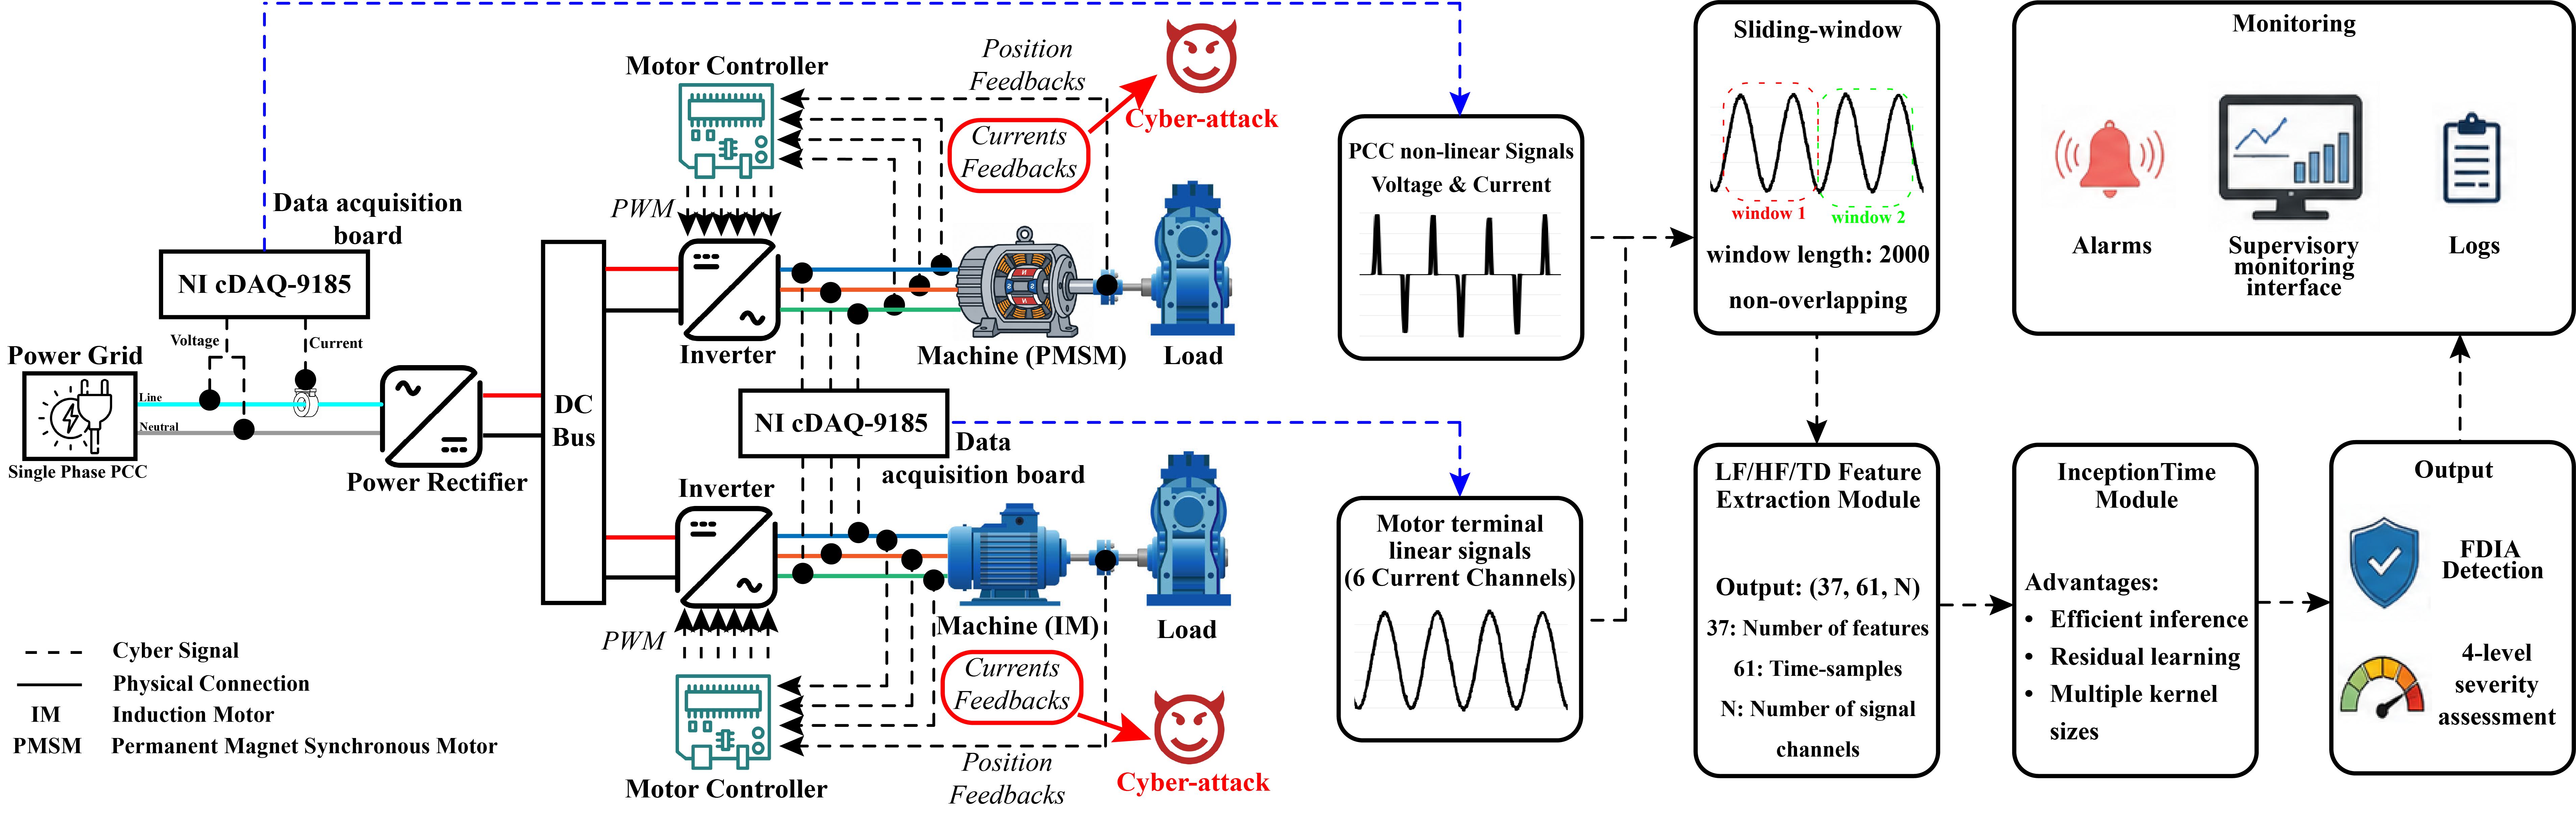
\includegraphics[width=0.95\textwidth]{figs/diagram2.png}
    \caption{Experimental platform used to generate current-feedback FDIAs in a heterogeneous inverter-fed motor-drive testbed.}

    % \COMMENTYe{Ty to draw a big picture for the framework. you can draw a diagram based on this picture}    

    
    \label{fig:system_schematic}
\end{figure*}

\subsection{Attack Model, Sensing Assumptions, and Labels}
\label{sec:attack_labels}

In the testbed, the FDIA is injected into the controller's phase-current feedback path. The PCC and motor-side monitoring sensors are used as trusted measurements to record the physical response of the drive system under attack. 
The monitoring sensors are isolated from the compromised controller feedback path. Thus, PCC sensing represents the nonintrusive monitoring case, while motor-side sensing serves as a performance reference. Replay, denial-of-service, monitoring-sensor attacks, and malicious command manipulation are outside the scope of this study.

Let $\mathbf{i}_{abc}(t)=[i_a(t),i_b(t),i_c(t)]^\top$ denote the true three-phase current-feedback vector, and let $\tilde{\mathbf{i}}_{abc}(t)$ denote the corrupted current-feedback vector received by the motor controller. During an attack interval, the FDIA is modeled as an additive phase-current bias:
\begin{equation}
\tilde{\mathbf{i}}_{abc}(t)
=
\mathbf{i}_{abc}(t)+\boldsymbol{\alpha},
\qquad t\in[t_{\mathrm{on}},t_{\mathrm{off}}],
\label{eq:fdia_model}
\end{equation}
Here, \(\boldsymbol{\alpha}=[\alpha_a,\alpha_b,\alpha_c]^\top\) denotes the injected per-unit bias vector, with \(\boldsymbol{\alpha}=\mathbf{0}\) outside the attack interval. The tested nonzero bias magnitudes range from \(0.0005\) to \(0.0050~\mathrm{pu}\), corresponding to \(0.05\%\)--\(0.5\%\) current-feedback bias. These low-severity FDIAs are difficult to detect because their signatures can be masked by normal variation, harmonics, and PCC aggregation. Attack severity is measured by the largest injected phase-current bias, 
\(s=\|\boldsymbol{\alpha}\|_\infty\).

For binary FDIA detection, each window is labeled as
$y_{\mathrm{fdia2}}=1$ if $s>0$ and $y_{\mathrm{fdia2}}=0$ otherwise. 
For four-class severity assessment, the label is defined as
\begin{equation}
y_{\mathrm{severity4}} =
\begin{cases}
0, & s=0 \quad \text{(normal)},\\
1, & 0.0005 \leq s \leq 0.0015 \quad \text{(mild)},\\
2, & 0.0020 \leq s \leq 0.0035 \quad \text{(medium)},\\
3, & 0.0040 \leq s \leq 0.0050 \quad \text{(severe)}.
\end{cases}
\label{eq:severity_bins}
\end{equation}
corresponding to normal, mild, medium, and severe conditions, respectively.
Table~\ref{tab:cyberattack_dataset_structure} summarizes the swept single-phase, equal two-phase, and fixed-plus-swept two-phase FDIA cases. Across three speeds, three load settings, and two motor types, the dataset contains 540 total attack cases. Each recording consists of 30 consecutive 20-s episodes, with 10~s normal operation followed by 10~s FDIA operation.

\begin{table}[t]
\centering
\footnotesize
\caption{FDIA dataset structure.}
\label{tab:cyberattack_dataset_structure}
\renewcommand{\arraystretch}{1.12}
\begin{tabular}{c c c c}
\hline
Cases & Phases & Bias Pattern & Total \\
\hline
1--10  & A   & $\alpha_a$: $0.0005$--$0.0050$ & 180 \\
11--20 & A,B & $\alpha_a=\alpha_b$: $0.0005$--$0.0050$ & 180 \\
21--30 & A,B & $\alpha_a=0.0050$, $\alpha_b$: $0.0005$--$0.0050$ & 180 \\
\hline
\multicolumn{3}{r}{Overall} & 540 \\
\hline
\end{tabular}
\vspace{1mm}
\begin{flushleft}
\footnotesize Each case group is evaluated over 3 speeds, 3 load settings, and 2 motor types. For all cases, unspecified phase biases are zero.
\end{flushleft}
\end{table}


\subsection{Data Acquisition and Operating Conditions}
\label{sec:data_acquisition}

Electrical measurements were acquired from the testbed using a National Instruments cDAQ-9185 chassis and a custom data-collector interface board. The interface board routed synchronized motor-side and PCC-side analog channels to the acquisition system. Three brake-excitation settings were tested for each machine: 1--3~V for the ACIM branch and 2--4~V for the PMSM branch. Because torque was not directly measured, these brake-excitation voltages are used as load-condition labels. All channels were sampled at 10~kHz and stored in TDMS format. For learning-based analysis, each record was segmented into non-overlapping 0.2~s windows containing 2{,}000 samples. This non-overlapping segmentation prevents temporal leakage before train/validation/test splitting. The resulting dataset dimensions, input configurations, severity-label distributions, and evaluation protocols are summarized in Table~\ref{tab:evaluation_protocols}.

\begin{figure*}[t]
    \centering
    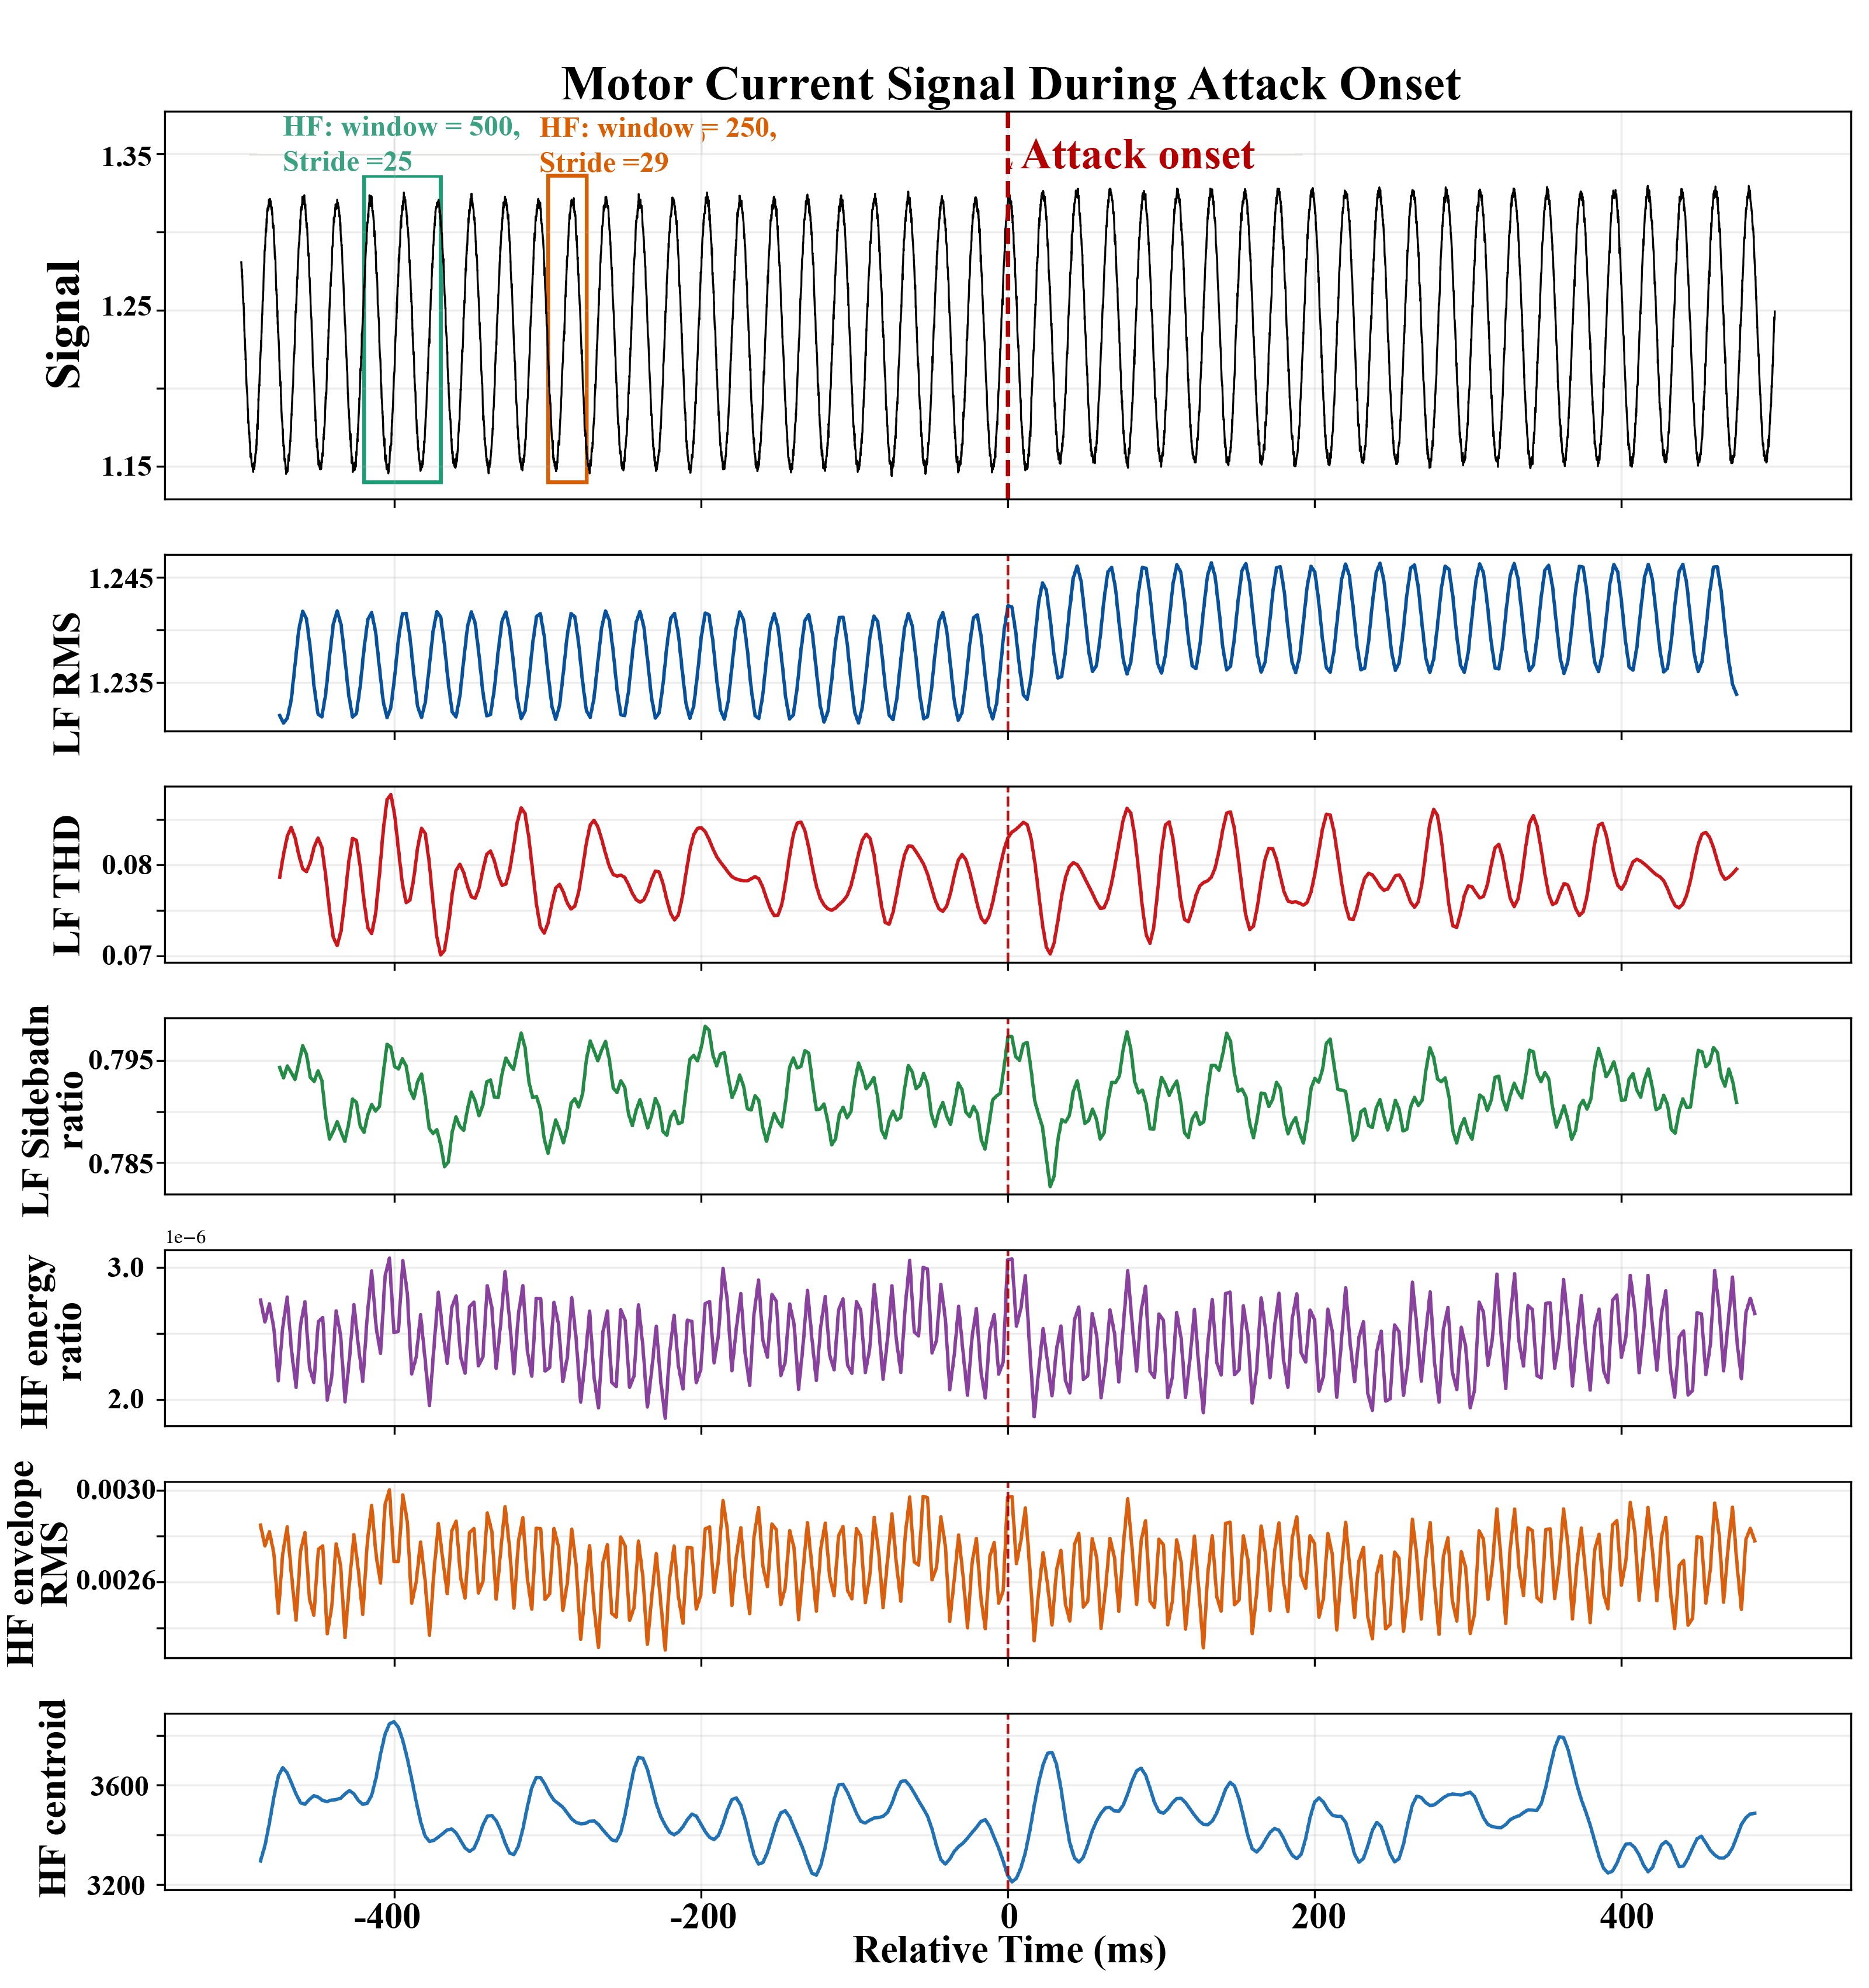
\includegraphics[width=0.49\textwidth]{figs/tdms_lfhf_window_example_acim_179p9s_separate_revised.png}
    \hfill
    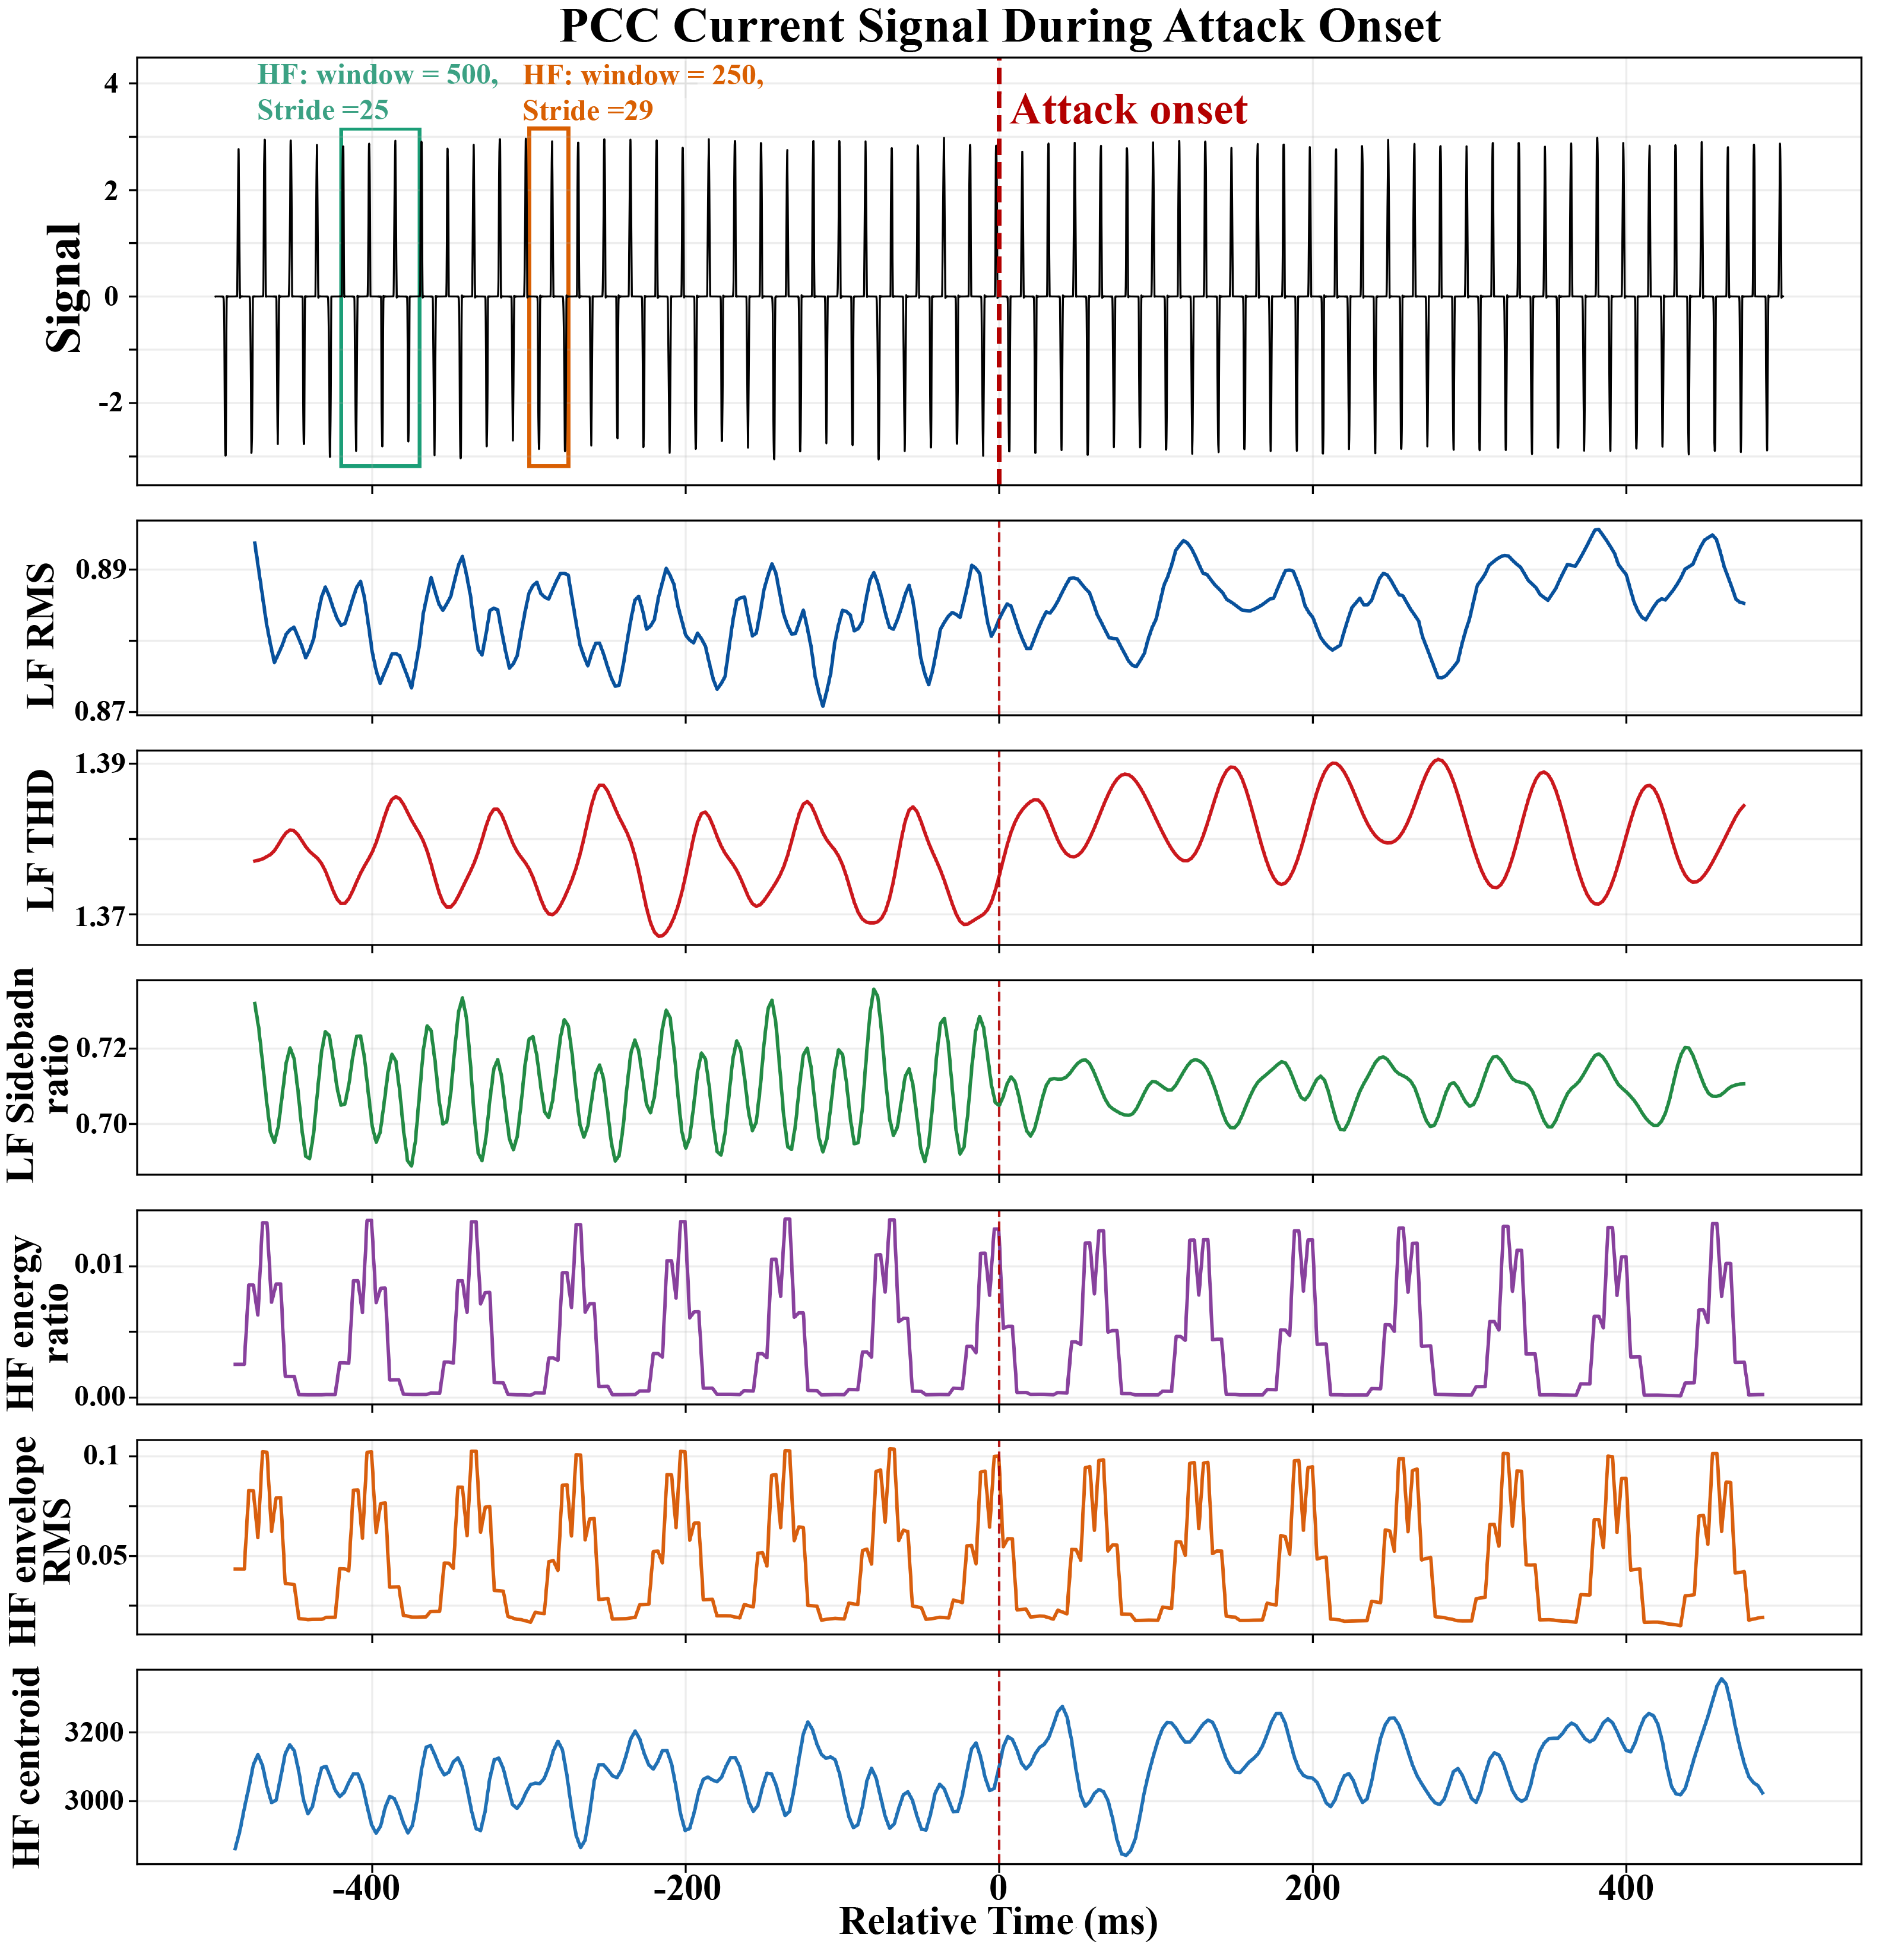
\includegraphics[width=0.49\textwidth]{figs/tdms_lfhf_window_example_pcc_179p9s_separate_revised.png}
    \caption{Representative motor-side and PCC-side signals at attack onset with the corresponding LF/HF feature responses.}
    \label{fig:lfhf_motor_pcc_examples}
\end{figure*}

\begin{table}[t]
\centering
\caption{Measurement streams used for monitoring.}
\label{tab:measurement_streams}
\renewcommand{\arraystretch}{1.15}
\begin{tabular}{l c c}
\hline
Stream & Measured signals & Channels \\
\hline
Motor-side & ACIM and PMSM phase currents & 6 \\
PCC-side   & PCC voltage and current & 2 \\
\hline
\end{tabular}
\end{table}                       

\begin{table}[t]
\centering
\caption{Dataset dimensions and evaluation protocols.}
\label{tab:evaluation_protocols}
\footnotesize
\renewcommand{\arraystretch}{1.15}
\setlength{\tabcolsep}{3.5pt}
\begin{tabularx}{\columnwidth}{@{}p{0.38\columnwidth}X@{}}
\toprule
\textbf{Parameter} & \textbf{Value / Configuration} \\
\hline
\multicolumn{2}{c}{\textit{Data dimensions}} \\
\hline
Total samples       & 60,054 \\
Motor distribution  & ACIM: 30,204; PMSM: 29,850 \\
Binary distribution & Normal: 33,054; Attack: 27,000 \\

\hline
\multicolumn{2}{c}{\textit{Input configuration}} \\
\hline
Time steps per sample, $W$ & 61 \\
Features per channel       & 37 \\
Channels                   & Motor: 6; PCC: 2 \\
Motor feature shape         & $(N,W,F)=(N,61,222)$ \\
PCC feature shape           & $(N,W,F)=(N,61,74)$ \\
\hline
\multicolumn{2}{c}{\textit{Severity labels}} \\
\hline
Raw severity levels & $0\%, 0.05\%, 0.1\%, \ldots, 0.5\%$ \\
Four-class labels   & Normal: 33,054; Mild: 8,100; Medium: 10,800; Severe: 8,100 \\

\hline
\multicolumn{2}{c}{\textit{Protocol 1: In-domain evaluation}} \\
\hline
Split ratio    & Train / validation / test = 70\% / 15\% / 15\% \\
Sample counts  & 42,037 / 9,008 / 9,009 \\
Domain composition & ACIM and PMSM samples appear in all splits \\

\hline
\multicolumn{2}{c}{\textit{Protocol 2: Cross-domain evaluation}} \\
\hline
Transfer directions & ACIM $\rightarrow$ PMSM; PMSM $\rightarrow$ ACIM \\
Adaptation ratios   & 1\%, 5\%, 10\%, and 20\% labeled target data \\
Reporting           & Three seeds; accuracy and balanced accuracy \\

\bottomrule
\end{tabularx}
\end{table}

\section{The Proposed Method}
\label{sec:method}

\subsection{LF/HF Feature Extraction Pipeline}
\label{sec:lfhf_features}


To represent both slow electromechanical behavior and faster attack-induced disturbances, a two-scale LF/HF feature pipeline was applied independently to each current channel. For every sample, a 2{,}000-point outer window was first extracted from the raw 10~kHz recording. Within this outer window, two parallel sliding analyses were performed. The LF branch uses a 500-sample window with a stride of 25 samples, while the HF branch uses a 250-sample window with a stride of 29 samples. The LF and HF settings both produce 61 time steps, enabling concatenation into one temporal feature tensor. 
Fig.~\ref{fig:lfhf_motor_pcc_examples} illustrates representative attack-onset responses and the corresponding LF/HF windows. In both cases, the raw signal is shown around the attack-transition instant, and representative LF and HF windows are overlaid to illustrate the two-scale extraction procedure. The motor-side signals exhibit stronger and more localized variations, whereas PCC-side responses are more distributed due to their aggregated nature.

% The full feature list is given in the Appendix. 
In total, 37 features were extracted per channel, including 18 LF spectral features, 11 HF spectral/envelope features, and 8 TD features. The LF branch targets slow electromechanical changes, fundamental-frequency behavior, harmonic distortion, sideband effects, and low-band energy redistribution. The HF branch captures higher-frequency redistribution and envelope-related changes that may appear during small current-feedback FDIAs. The TD features provide complementary sensitivity to amplitude variation, impulsiveness, waveform asymmetry, and short-term signal complexity.
Together, these features make weak PCC FDIA signatures more separable despite harmonics, grid interaction, and aggregation.

\subsection{Inception-Based Detection Model}
\label{sec:inception_model}

The extracted LF/HF tensors were modeled using a one-dimensional InceptionTime architecture~\cite{fawaz2020inceptiontime} for multivariate time-series classification. The input dimension is $(61,222)$ for the motor stream and $(61,74)$ for the PCC stream. As illustrated in Fig.~\ref{fig:inceptiontime_architecture}, the network uses bottleneck compression, parallel one-dimensional convolutional kernels, residual shortcuts, global average pooling, and a dense output layer. Motor and PCC models used stream-specific hyperparameters selected by validation balanced accuracy. The Inception-based design is well suited to the proposed LF/HF representation because the extracted features retain temporal ordering across the 61-step sequence. This preserves temporal interactions among LF, HF, and TD features.

\begin{figure*}[t]
    \centering
    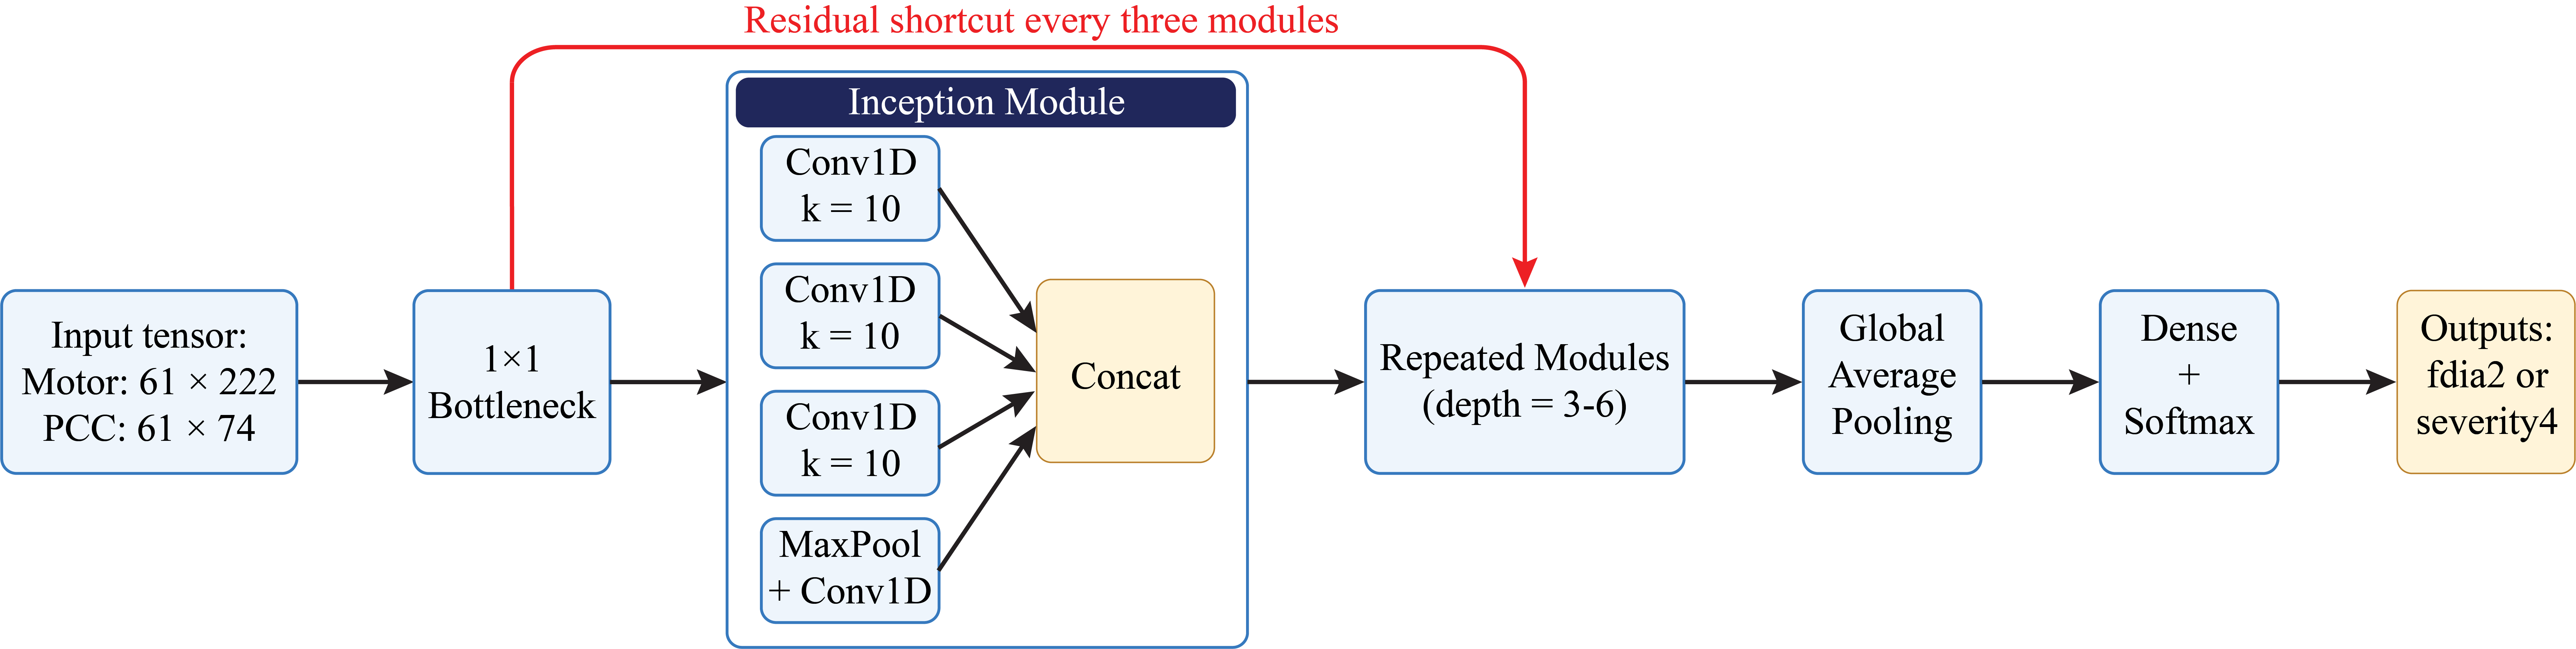
\includegraphics[width=0.95\textwidth]{figs/inceptiontime_architecture_lfhf.png}
    \caption{Overview of the InceptionTime-based classifier used for \texttt{fdia2} detection and \texttt{severity4} classification.}
    \label{fig:inceptiontime_architecture}
\end{figure*}

\subsection{Architecture of Online FDIA Detection and Attack-Severity Estimation}
\label{sec:AnomalyDetection}
The proposed pipeline supports online monitoring from trusted motor-terminal or PCC current measurements. Figure~\ref{fig:Online-algorithem} illustrates the overall architecture of the proposed monitoring pipeline. In the deployed setting, fixed-length windows of current data are acquired from either the motor terminals or the PCC, passed through the LF/HF feature-extraction stage, and then evaluated by the selected learning model to produce anomaly or severity decisions. The measurement, feature-extraction, and inference stages are modular, allowing the same pipeline to operate with motor-side or PCC inputs and supporting feature pruning, reduced-input models, and cross-motor adaptation. The framework provides alarms, severity indicators, and logs for supervisory systems; automatic mitigation is outside the scope. The same architecture is used for binary detection and severity classification. Binary detection is the primary PCC deployment task; severity estimates provide secondary diagnostic information. The experimental results in later sections show that motor-terminal sensing provides cleaner discriminative signatures, whereas PCC sensing offers a less intrusive sensing option for the tested setup.

\begin{figure*}[h]
\centering
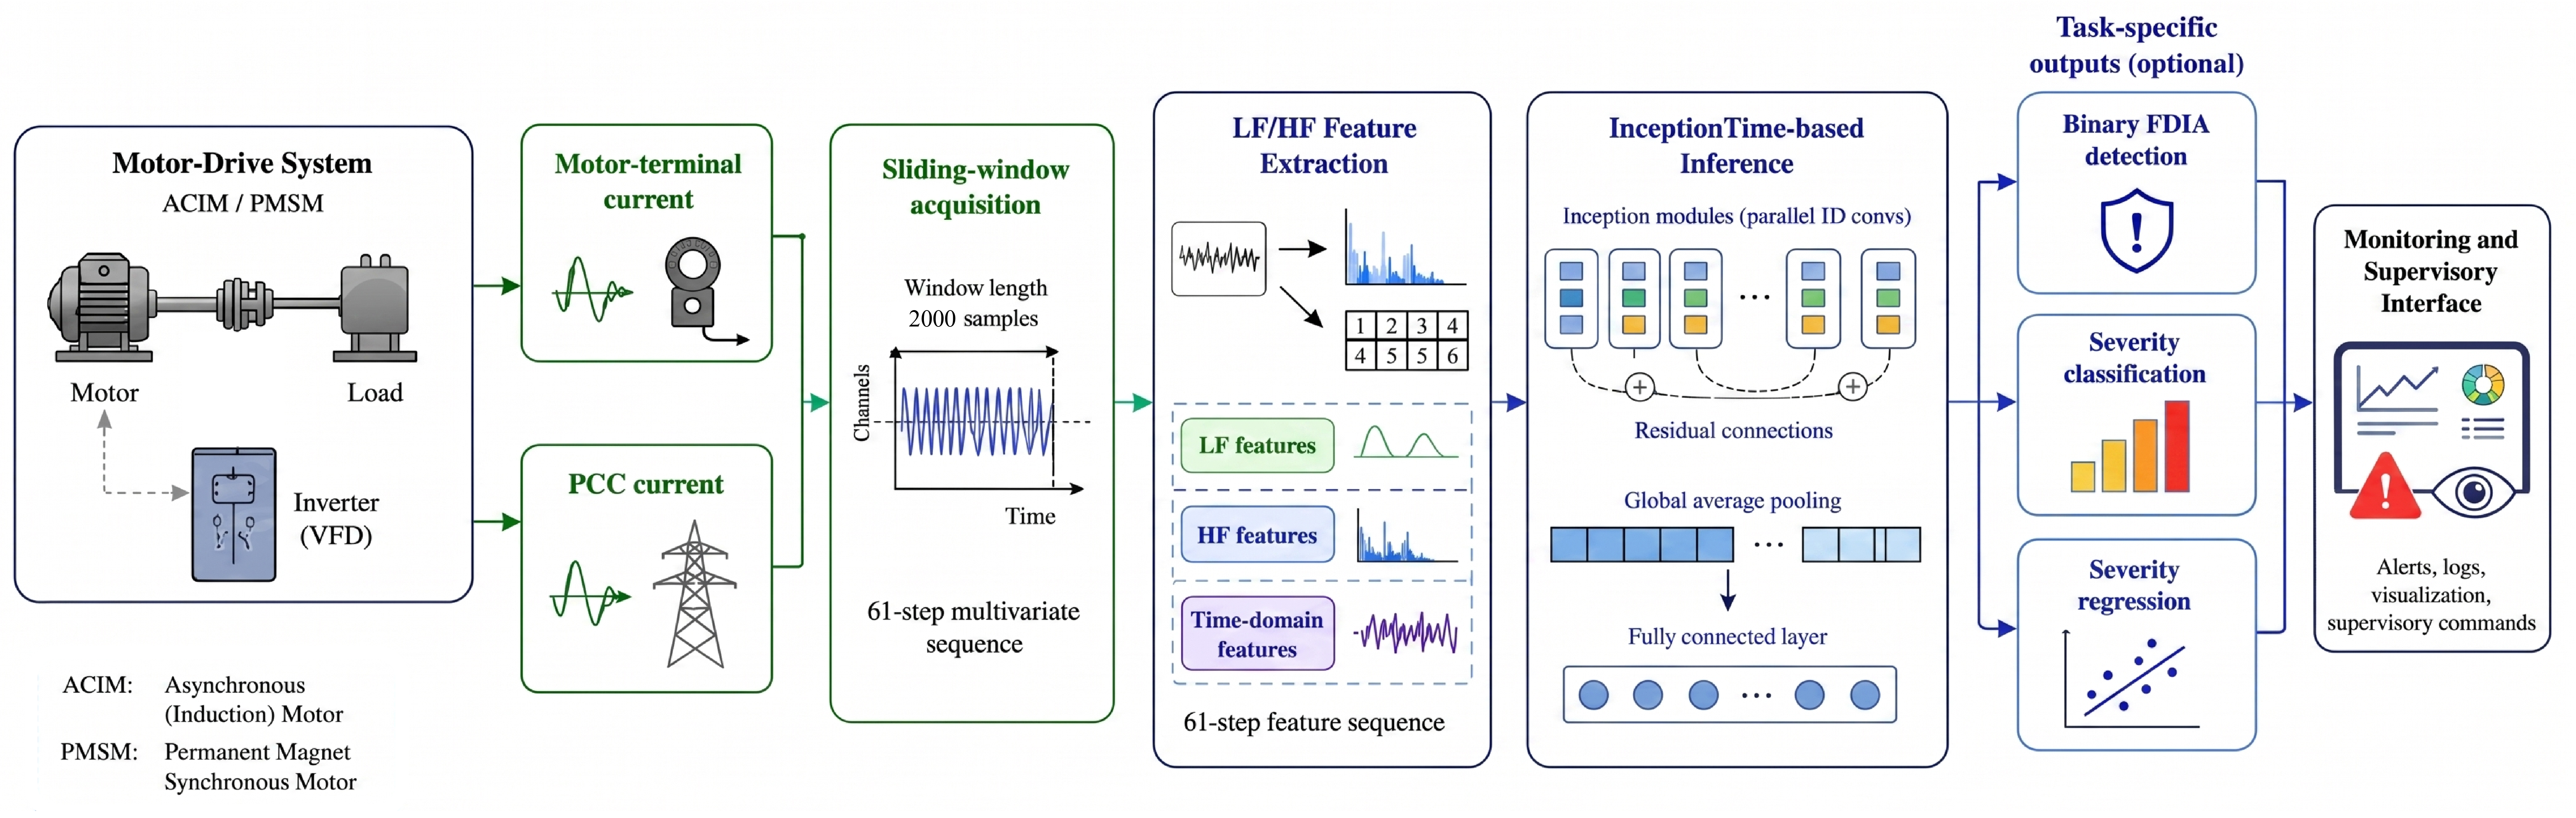
\includegraphics[width=0.99\linewidth]{figs/online_fdia_architecture.png}
\caption{Online FDIA detection and severity-assessment architecture for motor-side and PCC-side sensing.}
\label{fig:Online-algorithem}
\end{figure*}

\subsection{Training Details and Hyperparameters}
\label{sec:training_details}

For the InceptionTime-based models, hyperparameter selection was performed separately for the motor and PCC streams using validation-set balanced accuracy. The search varied depth, filters, bottleneck size, dropout, learning rate, weight decay, and batch size. Table~\ref{tab:search_top5_combined} summarizes the top-ranked configurations for both sensing streams.


\begin{table}[t]
\centering
\scriptsize
\caption{Top five InceptionTime configurations ranked by validation balanced accuracy on \texttt{severity4}.}
\label{tab:search_top5_combined}
\renewcommand{\arraystretch}{1.05}
\setlength{\tabcolsep}{2.5pt}
\begin{tabular}{c c c c c c c c c}
\hline
Rank & D & F & BN & Dr & LR & WD & BS & test BA (\%) \\
\hline
\multicolumn{9}{c}{\textit{Motor stream}} \\
\hline
1 & 3 & 32 & 16 & 0.20 & 0.0010 & $5{\times}10^{-5}$ & 128 & 98.25 \\
2 & 3 & 32 & 8  & 0.20 & 0.0010 & $10^{-4}$         & 64  & 98.08 \\
3 & 3 & 16 & 16 & 0.35 & 0.0010 & $5{\times}10^{-5}$ & 128 & 98.02 \\
4 & 3 & 32 & 8  & 0.20 & 0.0010 & $5{\times}10^{-5}$ & 128 & 97.99 \\
5 & 3 & 32 & 8  & 0.35 & 0.0010 & $10^{-4}$         & 64  & 97.96 \\
\hline
\multicolumn{9}{c}{\textit{PCC stream}} \\
\hline
1 & 6 & 32 & 32 & 0.20 & 0.0010 & $10^{-4}$         & 128 & 80.22 \\
2 & 6 & 48 & 8  & 0.20 & 0.0005 & $5{\times}10^{-5}$ & 128 & 79.95 \\
3 & 3 & 48 & 32 & 0.35 & 0.0005 & $5{\times}10^{-5}$ & 64  & 79.84 \\
4 & 4 & 32 & 32 & 0.35 & 0.0005 & $10^{-4}$         & 64  & 79.56 \\
5 & 4 & 48 & 32 & 0.50 & 0.0010 & $10^{-4}$         & 128 & 79.40 \\
\hline
\end{tabular}
\vspace{1mm}
\begin{flushleft}
\scriptsize D: depth; F: filters; BN: bottleneck; Dr: dropout; LR: learning rate; WD: weight decay; BS: batch size; test BA: test balanced accuracy.
\end{flushleft}
\end{table}

\subsection{Domain Adaptation Strategy: Source-Only vs Few-Shot Fine-Tuning}
\label{sec:domain_adaptation}
Few-shot adaptation was evaluated by training on one motor type and testing on the other. Two transfer directions were considered: ACIM $\rightarrow$ PMSM and PMSM $\rightarrow$ ACIM. For each direction, the detector was first trained using labeled data from the source motor only and then evaluated directly on the target motor. This \emph{source-only} setting quantifies cross-motor domain shift.

For adaptation, the source-trained model was fine-tuned using a small labeled subset of target-domain samples before testing on held-out target data. The target adaptation ratios considered in this work were 1\%, 5\%, 10\%, and 20\% of the available target-domain adaptation pool.
The domain-adaptation strategy was implemented as supervised fine-tuning rather than unsupervised feature alignment. Accordingly, all reported adaptation gains reflect the benefit of limited labeled target-domain data under a practical transfer-learning setting. To ensure reliable comparison, all cross-domain experiments were repeated over three random seeds, and the results were reported using both accuracy and balanced accuracy.

This protocol is particularly important in the present study because ACIM and PMSM signals exhibit substantial domain differences despite being collected under the same FDIA framework. This tests whether the LF/HF-Inception representation can be adapted with limited target-domain labels.
\section{Experimental Results}
\label{sec:results}
\subsection{In-Domain Baselines: Motor vs PCC}
\label{sec:in_domain}

Table~\ref{tab:all_tasks_in_domain} reports mixed-domain in-domain performance with ACIM and PMSM samples in all splits. The results show that motor-side sensing provides more discriminative attack signatures than PCC sensing for both (\texttt{fdia2}) and (\texttt{severity4}). In addition, (\texttt{severity4}) is substantially more challenging than binary attack detection, especially at PCC.

Thus, PCC-side severity estimates should be treated as coarse diagnostics, whereas motor-side measurements support finer severity discrimination. Overall, PCC monitoring is more challenging than motor-side monitoring, and severity assessment is harder than binary detection. These baseline findings motivate the subsequent cross-domain analysis, where the additional challenge of motor-type shift is introduced.

\begin{table}[t]
\centering
\caption{In-domain performance under the mixed ACIM/PMSM split.}
\label{tab:all_tasks_in_domain}
\renewcommand{\arraystretch}{1.15}
\setlength{\tabcolsep}{4pt}
\begin{tabular}{l c c c c c}
\hline
Task & Accuracy & Bal. Acc. & Precision & Recall & F1 \\
     & (\%)    & Accuracy (\%)      & (\%)   & (\%)   & (\%) \\
\hline
\multicolumn{6}{c}{\textit{PCC stream}} \\
\hline
\texttt{fdia2}      & 89.44 & 88.99 & 89.71 & 88.99 & 89.25 \\
\texttt{severity4}  & 84.17 & 80.22 & 80.50 & 80.22 & 80.32 \\
Motor type          & 100.00 & 100.00 & 100.00 & 100.00 & 100.00 \\
\hline
\multicolumn{6}{c}{\textit{Motor stream}} \\
\hline
\texttt{fdia2}      & 98.89 & 98.85 & 98.91 & 98.85 & 98.88 \\
\texttt{severity4}  & 98.68 & 98.25 & 98.22 & 98.25 & 98.24 \\
Motor type          & 100.00 & 100.00 & 100.00 & 100.00 & 100.00 \\
\hline
\end{tabular}
\vspace{1mm}
\begin{flushleft}
\scriptsize Precision, recall, and F1 are reported as macro-averaged values in paper.
\end{flushleft}
\end{table}

\subsection{Comparison with Deep and Classical ML Baselines}
\label{sec:model_comparison}
To benchmark the proposed LF/HF Inception-based model, representative deep-learning and classical ML baselines were evaluated on the PCC-based \texttt{fdia2} and \texttt{severity4} tasks, which were the most challenging in-domain settings. The baselines include ResNet, MLSTM-FCN, Random Forest, and XGBoost, while the proposed model uses the final stream-specific InceptionTime configuration selected by validation-based hyperparameter search. As shown in Table~\ref{tab:model_comparison_hard_tasks}, the proposed model achieved the highest accuracy, balanced accuracy, and F1 score among the evaluated baselines on both PCC tasks. The performance gap is larger for \texttt{severity4}, confirming that PCC-based severity discrimination is more challenging than binary FDIA detection and benefits from the proposed temporal LF/HF representation.

\begin{table}[t]
\centering
\caption{Baseline comparison on the PCC-based \texttt{fdia2} and \texttt{severity4} tasks.}
\label{tab:model_comparison_hard_tasks}
\renewcommand{\arraystretch}{1.05}
\setlength{\tabcolsep}{3pt}
\begin{tabular}{l c c c}
\hline
Method & Acc. (\%) & Balanced Acc. (\%) & F1 (\%) \\
\hline
\multicolumn{4}{c}{\textit{\texttt{fdia2}}} \\
\hline
Proposed InceptionTime & 89.44 & 88.99 & 89.25 \\
ResNet        & 85.58 & 84.83 & 85.20 \\
MLSTM-FCN     & 84.58 & 83.80 & 84.17 \\
Rand. Forest  & 86.05 & 85.27 & 85.67 \\
XGBoost       & 86.45 & 85.75 & 86.11 \\
\hline
\multicolumn{4}{c}{\textit{\texttt{severity4}}} \\
\hline
Proposed InceptionTime & 84.17 & 80.22 & 80.32 \\
ResNet        & 77.31 & 70.22 & 70.68 \\
MLSTM-FCN     & 77.96 & 71.11 & 71.89 \\
Rand. Forest  & 83.42 & 72.68 & 77.40 \\
XGBoost       & 79.00 & 65.21 & 70.45 \\
\hline
\end{tabular}
\end{table}

\subsection{Cross-Domain Transfer Without Adaptation}
\label{sec:cross_domain}
Source-only transfer was evaluated by training on one motor type and testing directly on the other. Two transfer directions were considered: ACIM $\rightarrow$ PMSM and PMSM $\rightarrow$ ACIM. Table~\ref{tab:cross_domain_source_only} shows that source-only fdia2 transfer falls near chance balanced accuracy for both sensing streams. For \texttt{fdia2}, the source-only results in Table~\ref{tab:cross_domain_source_only} show a substantial degradation relative to the mixed-domain baselines. This confirms a substantial ACIM/PMSM domain shift in the tested transfer setting. Thus, reliable cross-motor FDIA detection in this setting benefits from target-domain adaptation.
\begin{table}[t]
\centering
\caption{Cross-domain source-only performance without target-domain adaptation on \texttt{fdia2} task.}
\label{tab:cross_domain_source_only}
\renewcommand{\arraystretch}{1.15}
\begin{tabular}{l l c c c c}
\hline
Stream & Direction & Accuracy (\%) & Balanced Acc. (\%) \\
\hline
Motor & ACIM $\rightarrow$ PMSM & 53.87 & 50.10 \\
Motor & PMSM $\rightarrow$ ACIM & 51.08 & 51.80 \\
PCC   & ACIM $\rightarrow$ PMSM & 54.79 & 50.07 \\
PCC   & PMSM $\rightarrow$ ACIM & 52.38 & 57.03 \\
\hline
\end{tabular}
\end{table}
\subsection{Domain Adaptation Results: 1/5/10/20\%}
\label{sec:adaptation_results}
Table~\ref{tab:domain_adaptation_anomaly2} reports fdia2 few-shot adaptation using 1\%, 5\%, 10\%, and 20\% labeled target data. In all cases, adaptation improved performance relative to the source-only setting, although the magnitude of the gain was strongly direction dependent. For ACIM-to-PMSM transfer, adaptation gives only modest gains, reaching 57.49\% balanced accuracy for motor sensing and 60.06\% for PCC at 20\% target data. For PMSM-to-ACIM transfer, adaptation is much stronger, reaching 86.10\% balanced accuracy for motor sensing and 91.16\% for PCC at 20\% target data.
Overall, the adaptation results show that few-shot target-domain fine-tuning can improve transfer performance, but the gains are strongly direction dependent and are much larger in the PMSM $\rightarrow$ ACIM direction. This asymmetry indicates that cross-motor FDIA adaptation cannot be treated as a symmetric transfer problem; in practice, the pretraining motor domain materially affects PCC deployment performance.

\begin{table}[t]
\centering
\scriptsize
\caption{Few-shot domain-adaptation results for \texttt{fdia2} using labeled target-domain fine-tuning. Values are mean test balanced accuracy (\%) over three seeds.}
\label{tab:domain_adaptation_anomaly2}
\renewcommand{\arraystretch}{1.15}
\begin{tabular}{l l c c c c c}
\hline
Stream & Direction & Source-only & 1\% & 5\% & 10\% & 20\% \\
\hline
Motor & ACIM $\rightarrow$ PMSM & 50.10 & 50.06 & 49.63 & 53.15 & 57.49 \\
Motor & PMSM $\rightarrow$ ACIM & 51.80 & 57.95 & 73.75 & 78.86 & 86.10 \\
PCC   & ACIM $\rightarrow$ PMSM & 50.07 & 51.79 & 55.51 & 57.47 & 60.06 \\
PCC   & PMSM $\rightarrow$ ACIM & 57.03 & 70.10 & 84.56 & 89.12 & 91.16 \\
\hline
\end{tabular}
\end{table}




\subsection{Error Analysis: Confusion Matrices and FP/FN Behavior}
\label{sec:error_analysis}
Fig.~\ref{fig:main_confusion_matrices} compares the in-domain confusion matrices for \texttt{fdia2} and \texttt{severity4}. For \texttt{fdia2}, motor-side sensing yields a strongly diagonal confusion matrix with low false-positive and false-negative rates of 0.75\% and 1.56\%, respectively, whereas PCC sensing increases these rates to 6.55\% and 15.46\% because the attack is observed only through the aggregated current response. For \texttt{severity4}, PCC errors concentrate between adjacent classes, especially normal/mild and mild/medium, indicating that PCC measurements retain coarse attack information but blur finer severity distinctions.

Fig.~\ref{fig:case1_30_motor_pcc_detection_examples} complements the aggregate confusion-matrix results by showing a representative ACIM detection sequence on a continuous experimental signal. Both sensing locations follow the scheduled normal/FDIA intervals, but the motor-side detector produces cleaner transitions than the PCC-side detector, especially near the first attack onset and low-severity FDIA intervals. These results indicate that motor-side measurements are more separable, while PCC measurements remain useful but less reliable for fine severity discrimination. 
% Auxiliary motor-type and regression diagnostics are provided in the Appendix.

\begin{figure*}[t]
    \centering

    \begin{minipage}{0.48\textwidth}
        \centering
        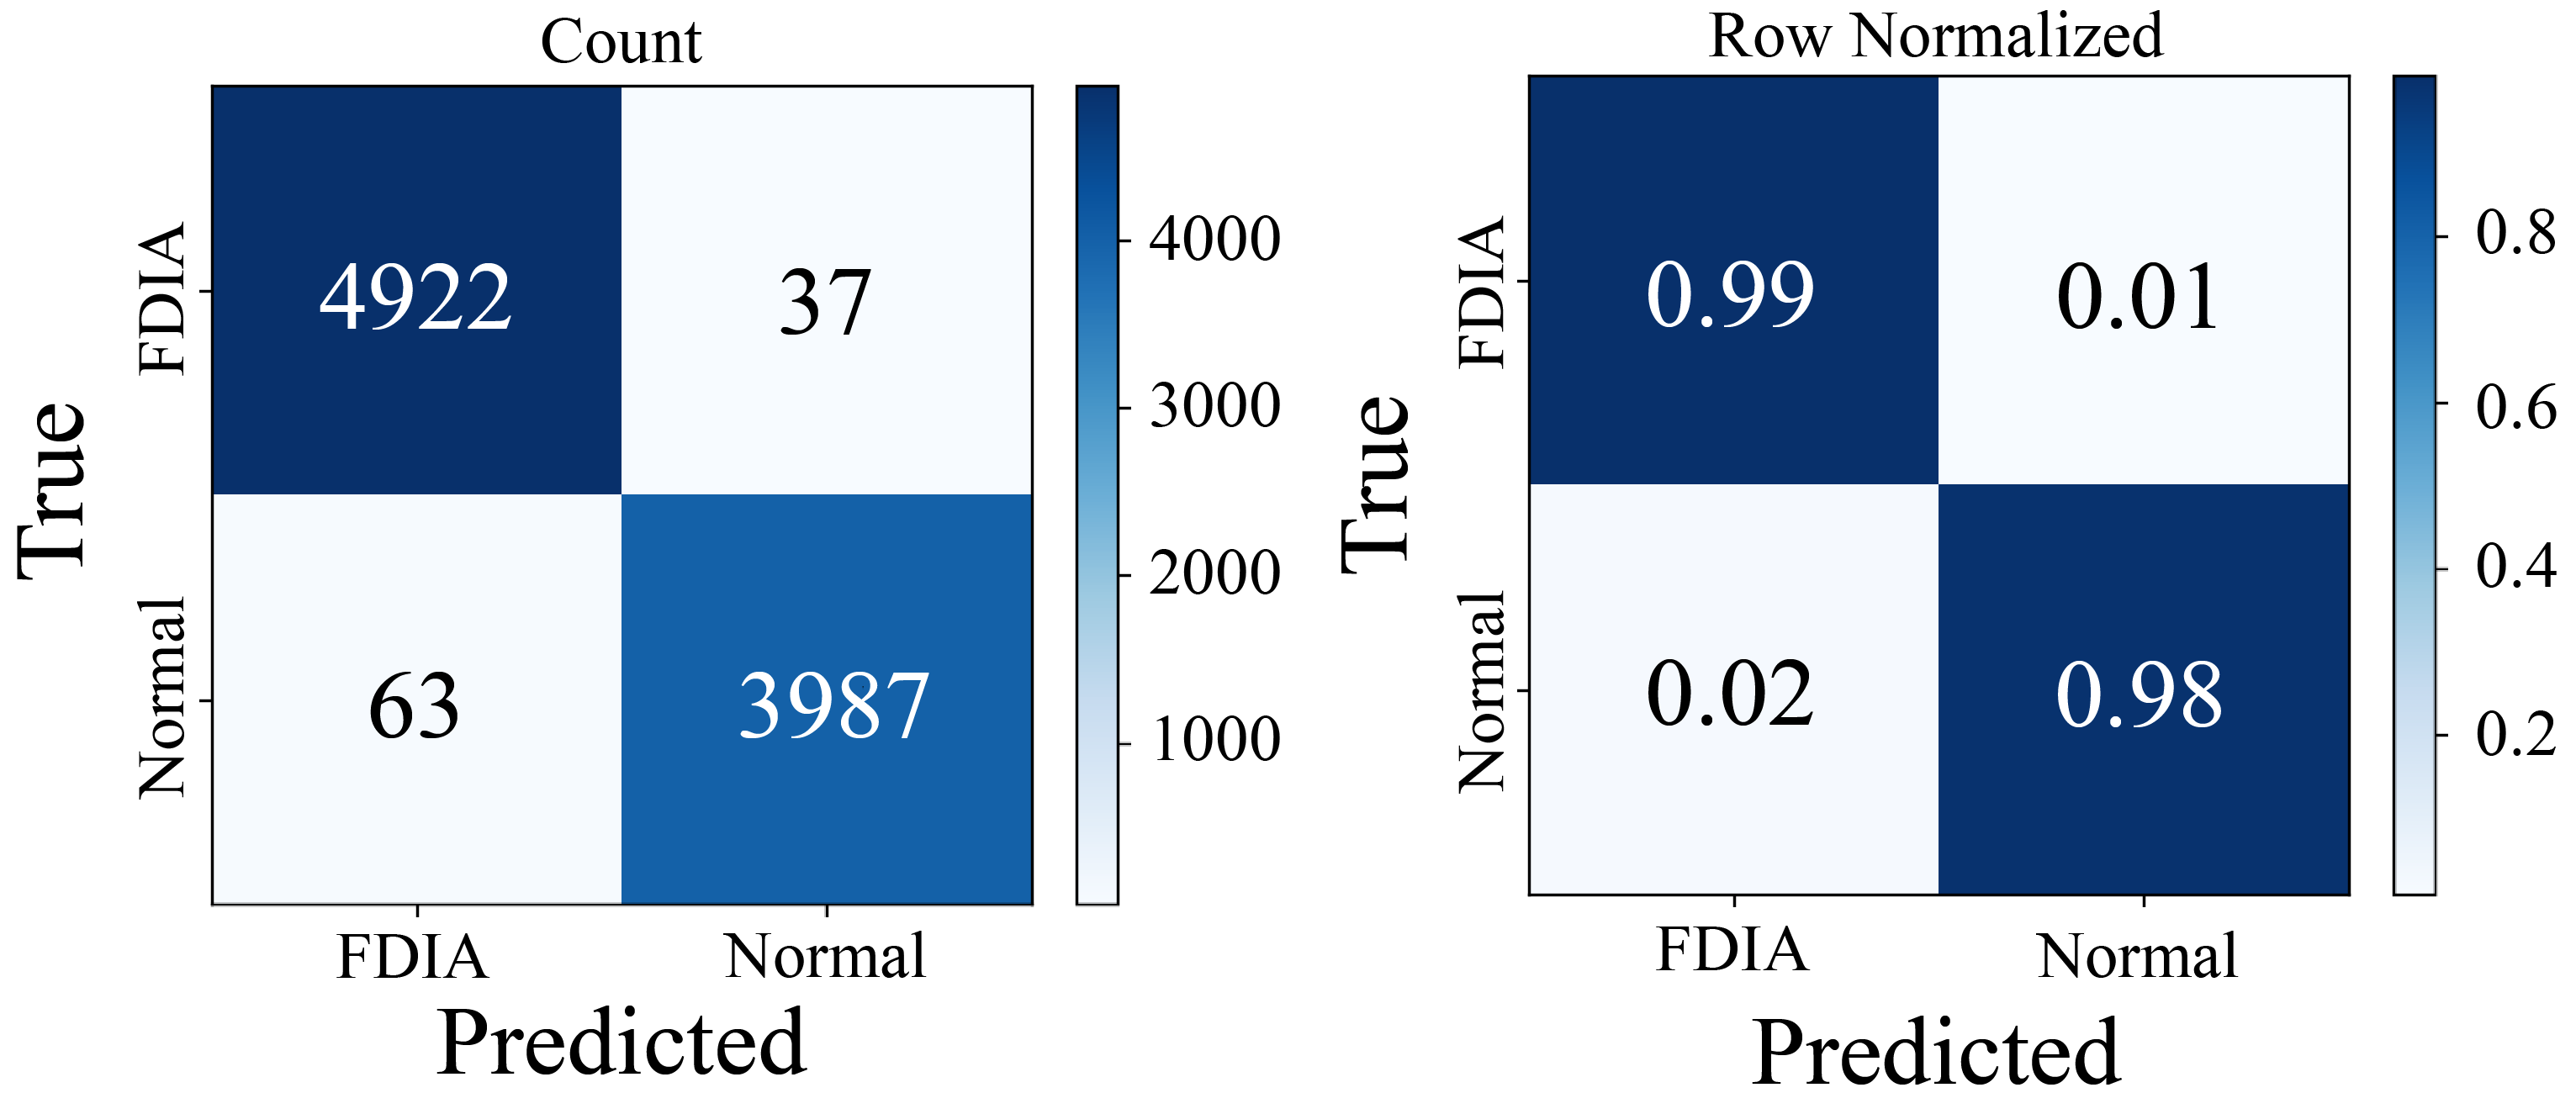
\includegraphics[width=\linewidth]{figs/anomaly2_motor_confusion_revised.png}
        \vspace{-1mm}
        \centerline{(a) \texttt{fdia2}, motor stream}
    \end{minipage}
    \hfill
    \begin{minipage}{0.48\textwidth}
        \centering
        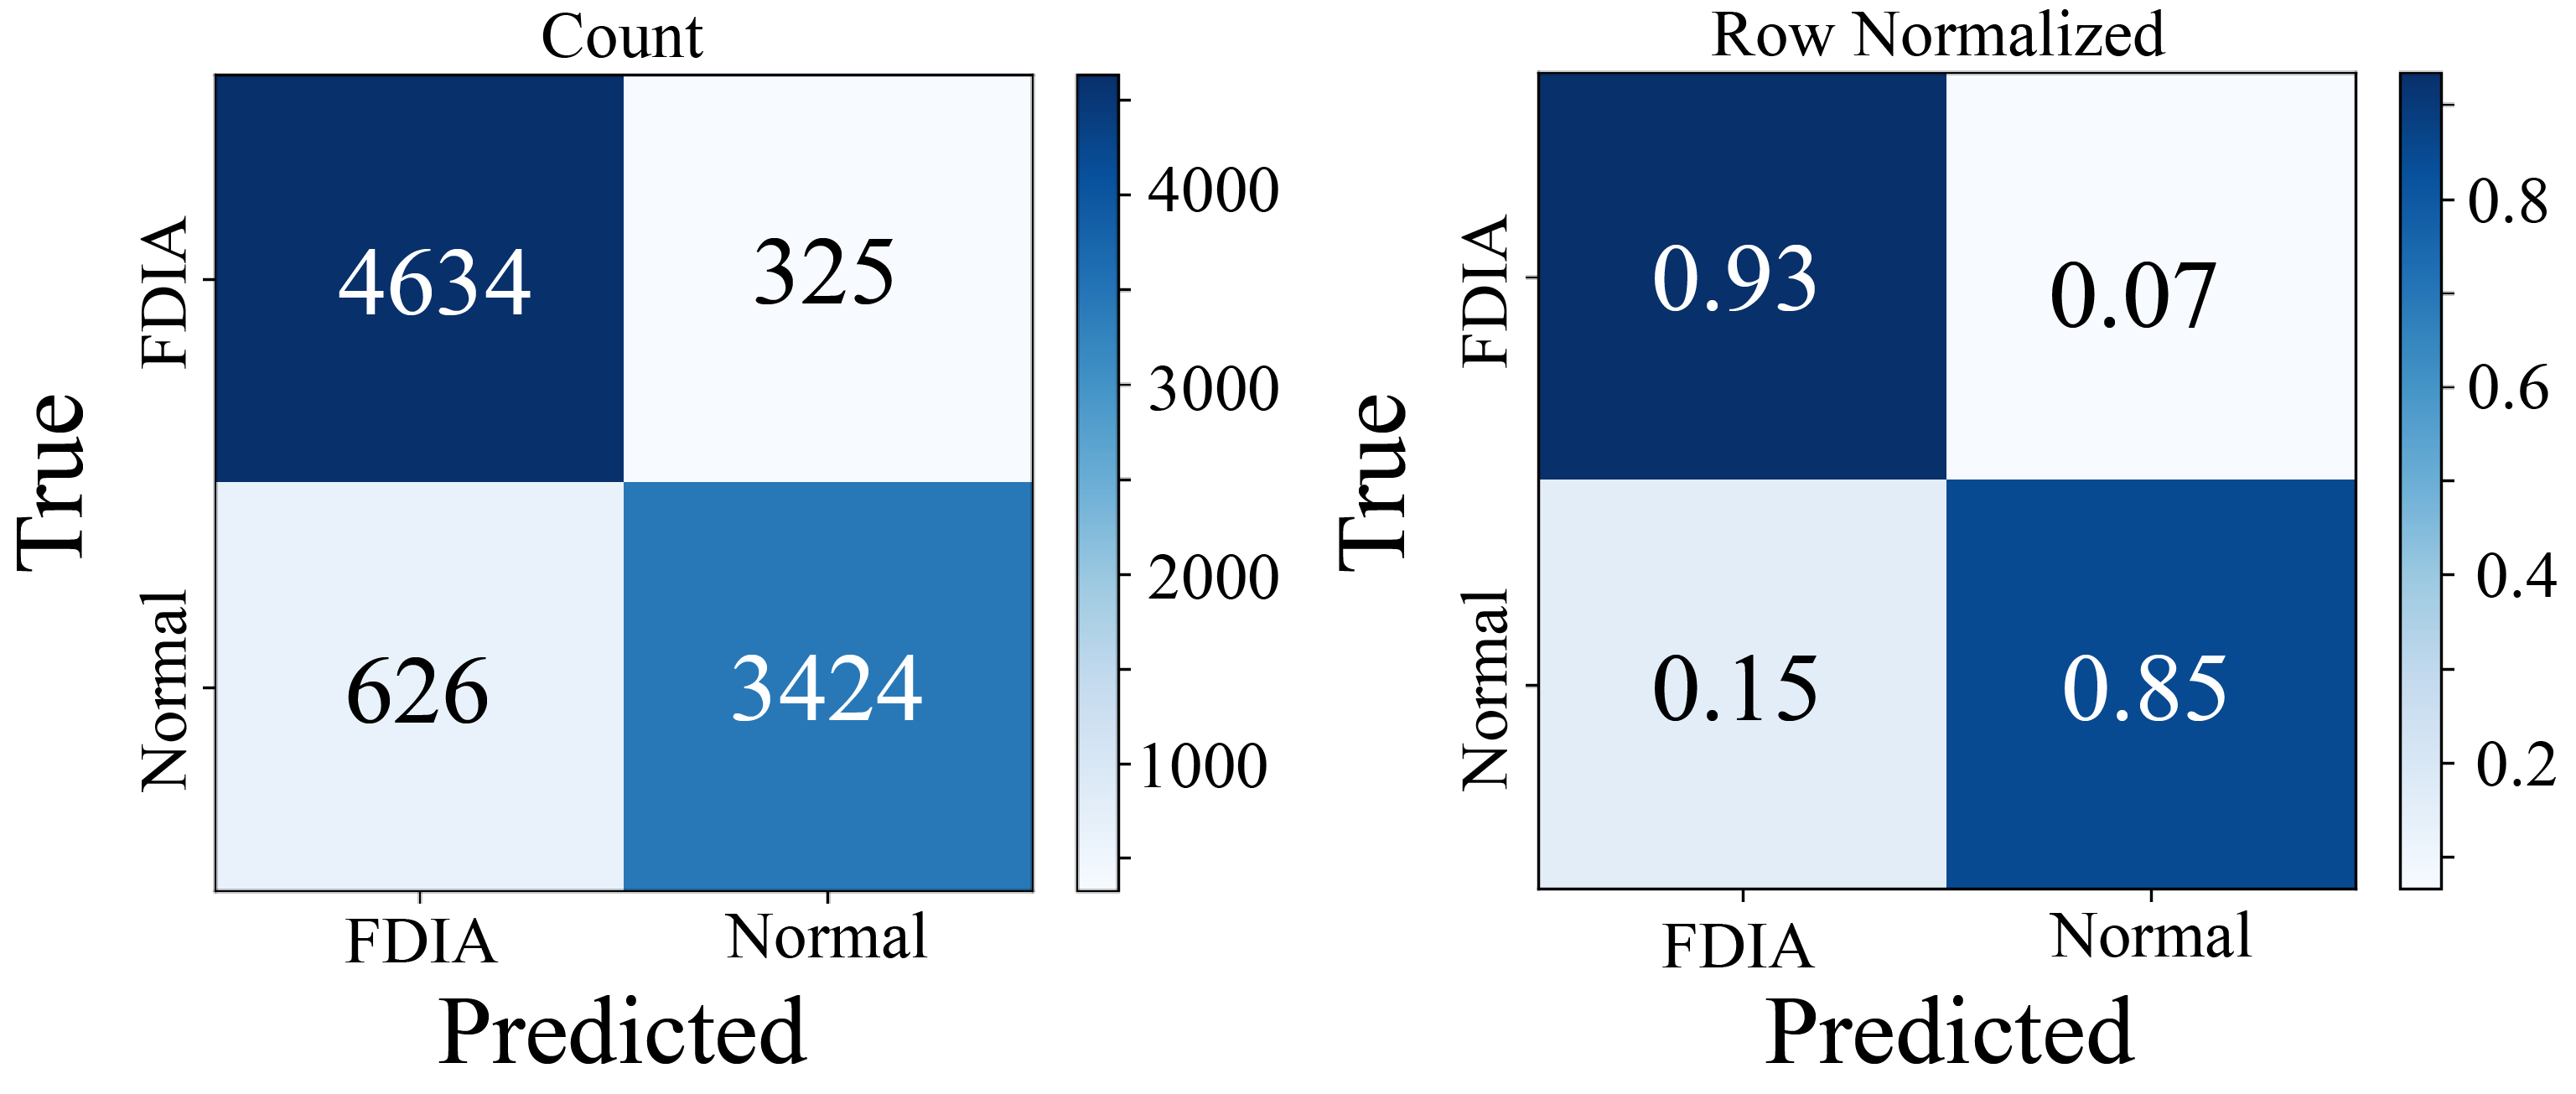
\includegraphics[width=\linewidth]{figs/anomaly2_pcc_confusion_revised.png}
        \vspace{-1mm}
        \centerline{(b) \texttt{fdia2}, PCC stream}
    \end{minipage}

    \vspace{2mm}

    \begin{minipage}{0.48\textwidth}
        \centering
        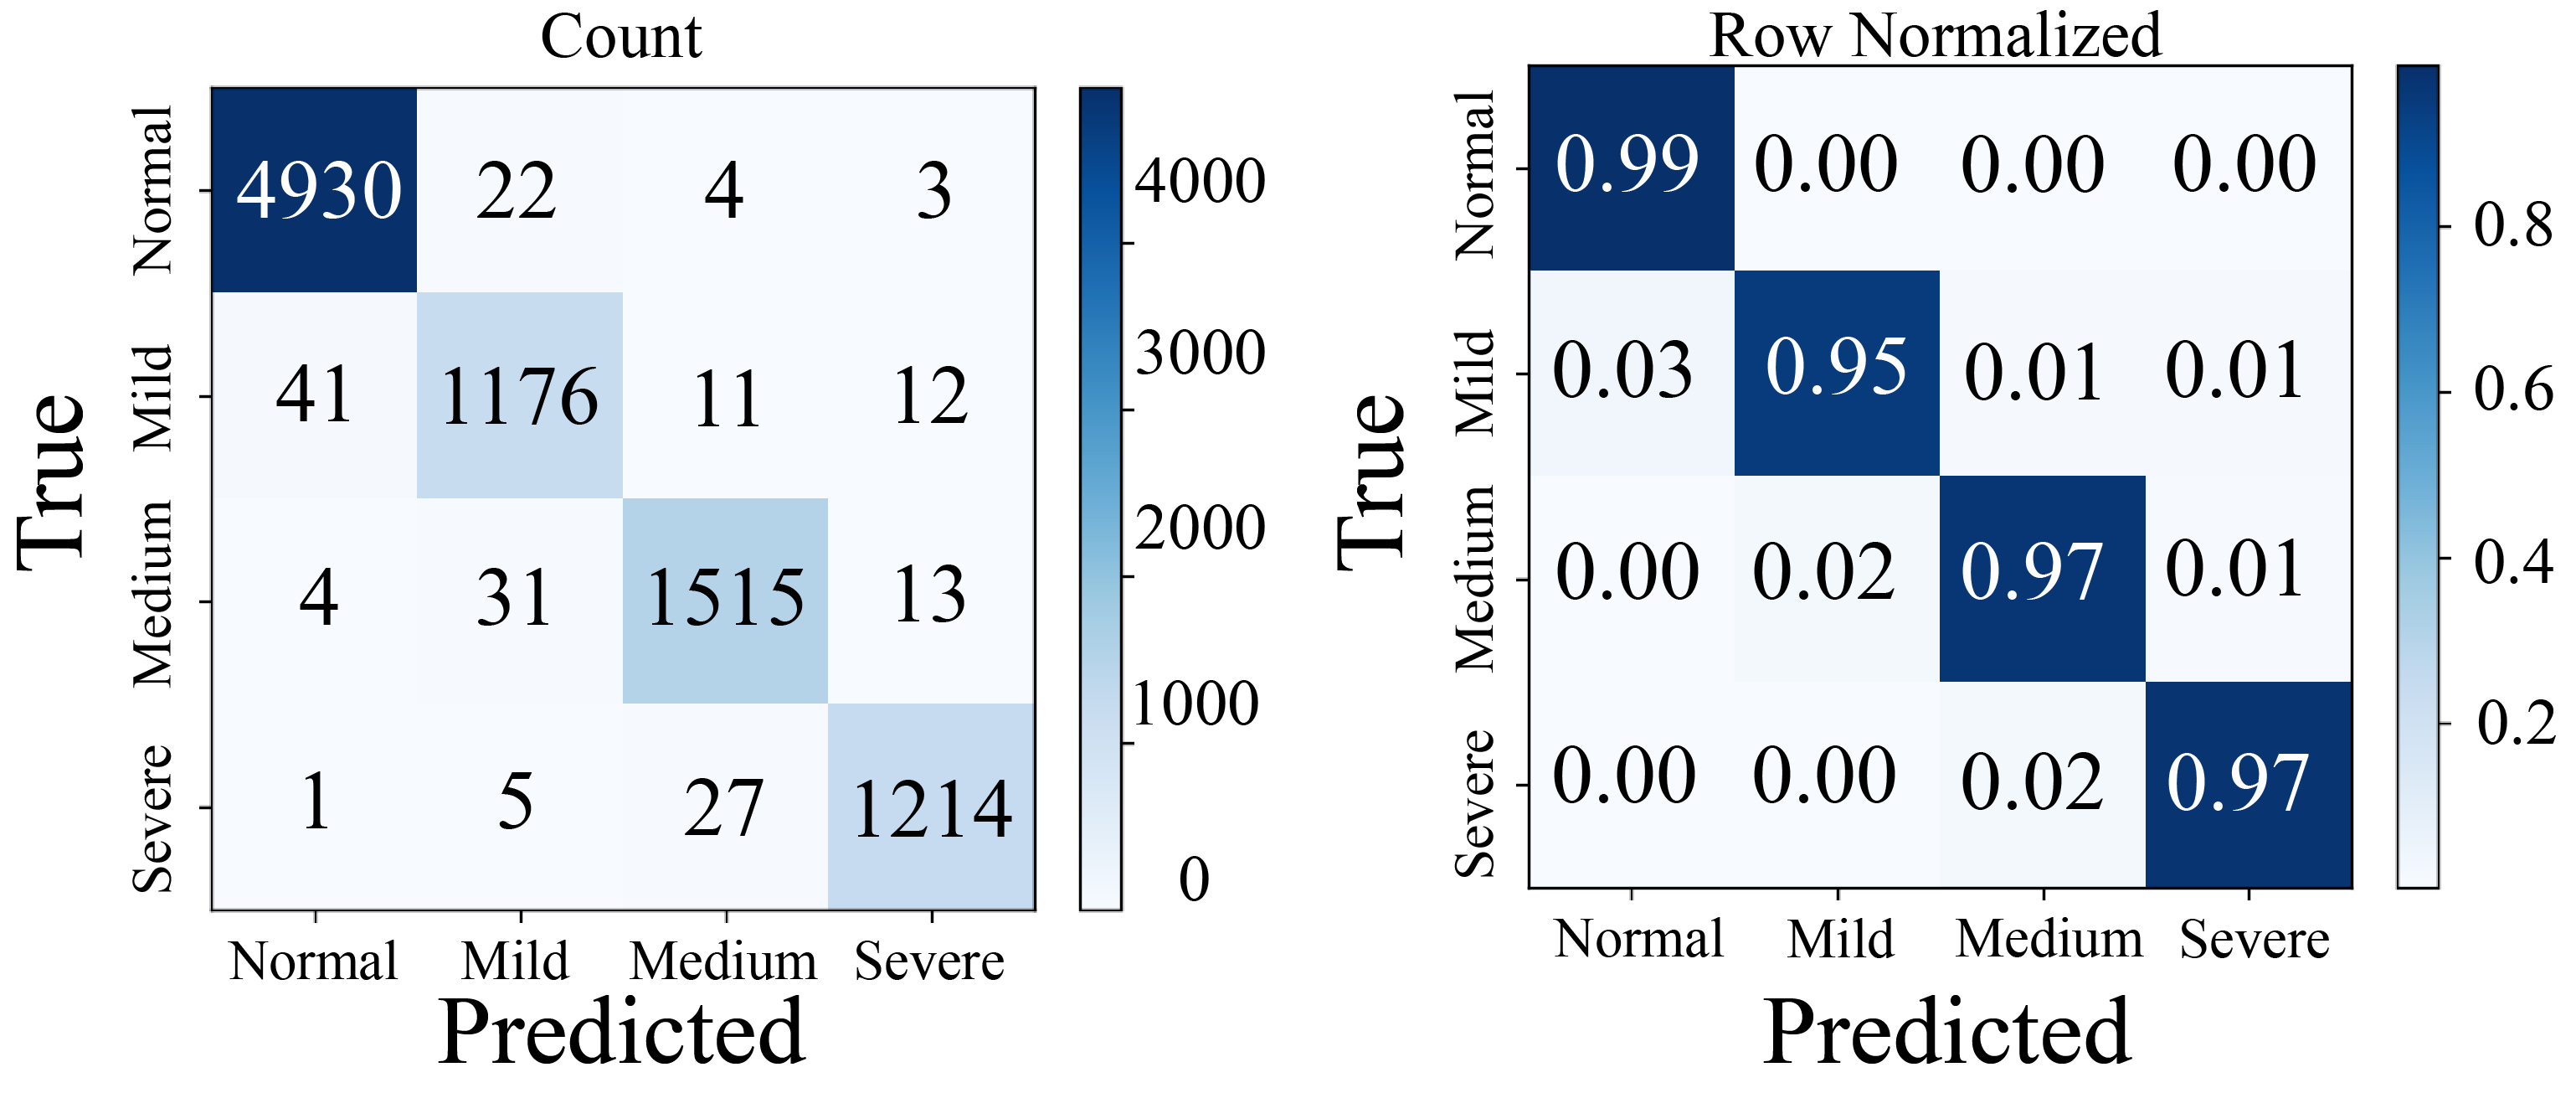
\includegraphics[width=\linewidth]{figs/severity4_motor_confusion_revised.png}
        \vspace{-1mm}
        \centerline{(c) \texttt{severity4}, motor stream}
    \end{minipage}
    \hfill
    \begin{minipage}{0.48\textwidth}
        \centering
        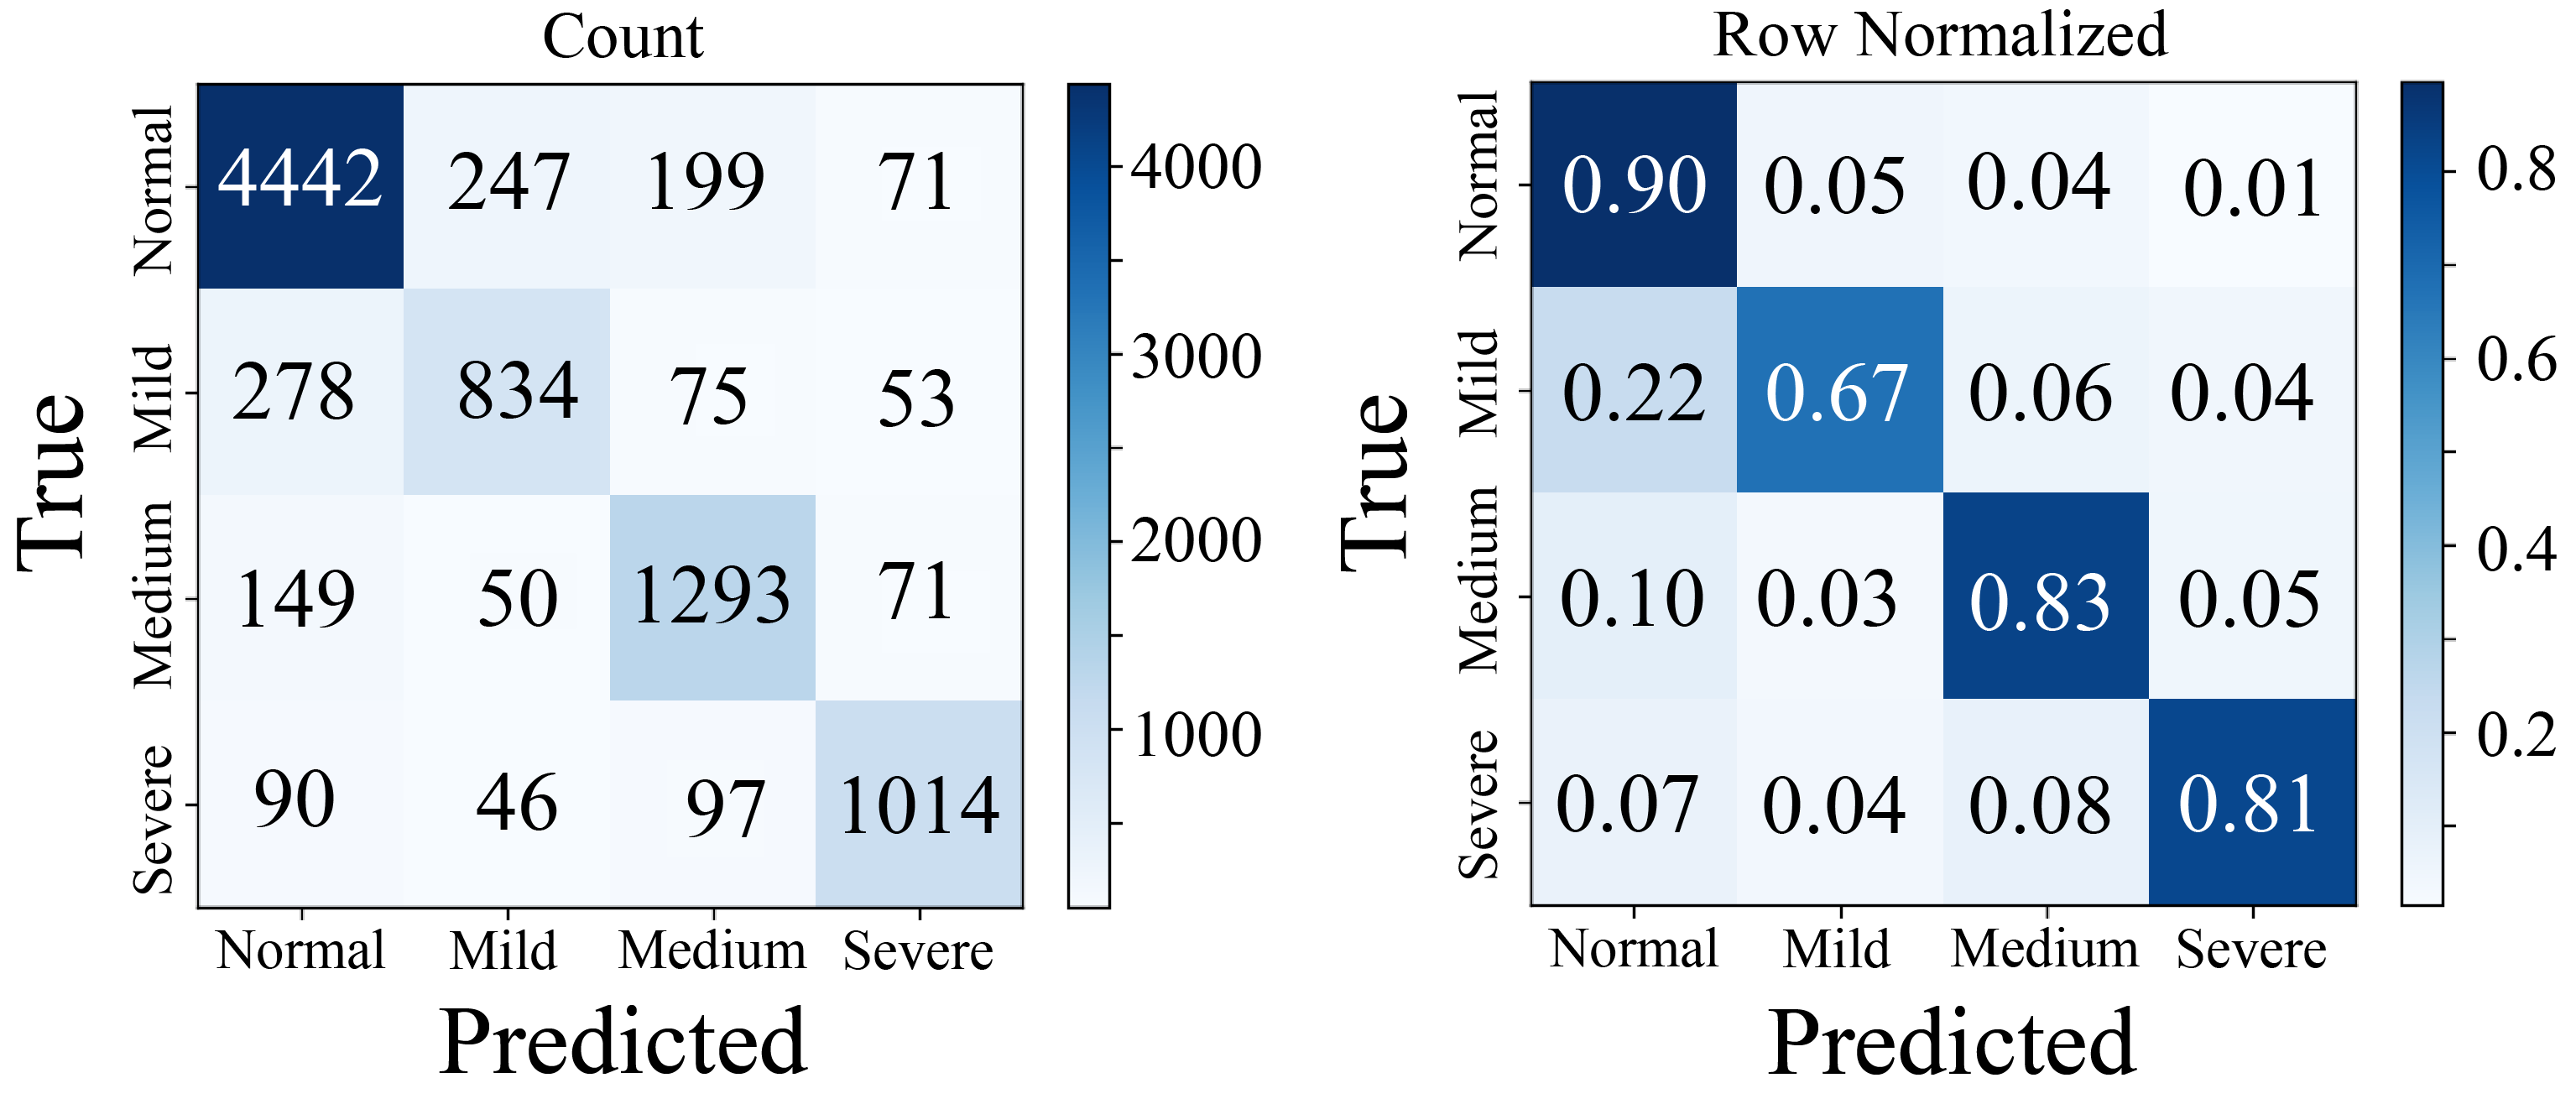
\includegraphics[width=\linewidth]{figs/severity4_pcc_confusion_revised.png}
        \vspace{-1mm}
        \centerline{(d) \texttt{severity4}, PCC stream}
    \end{minipage}

    \caption{In-domain confusion matrices for the proposed LF/HF InceptionTime classifier: (a) \texttt{fdia2} with motor-side measurements, (b) \texttt{fdia2} with PCC measurements, (c) \texttt{severity4} with motor-side measurements, and (d) \texttt{severity4} with PCC measurements.}
    \label{fig:main_confusion_matrices}
\end{figure*}
\begin{figure}[t]
    \centering
    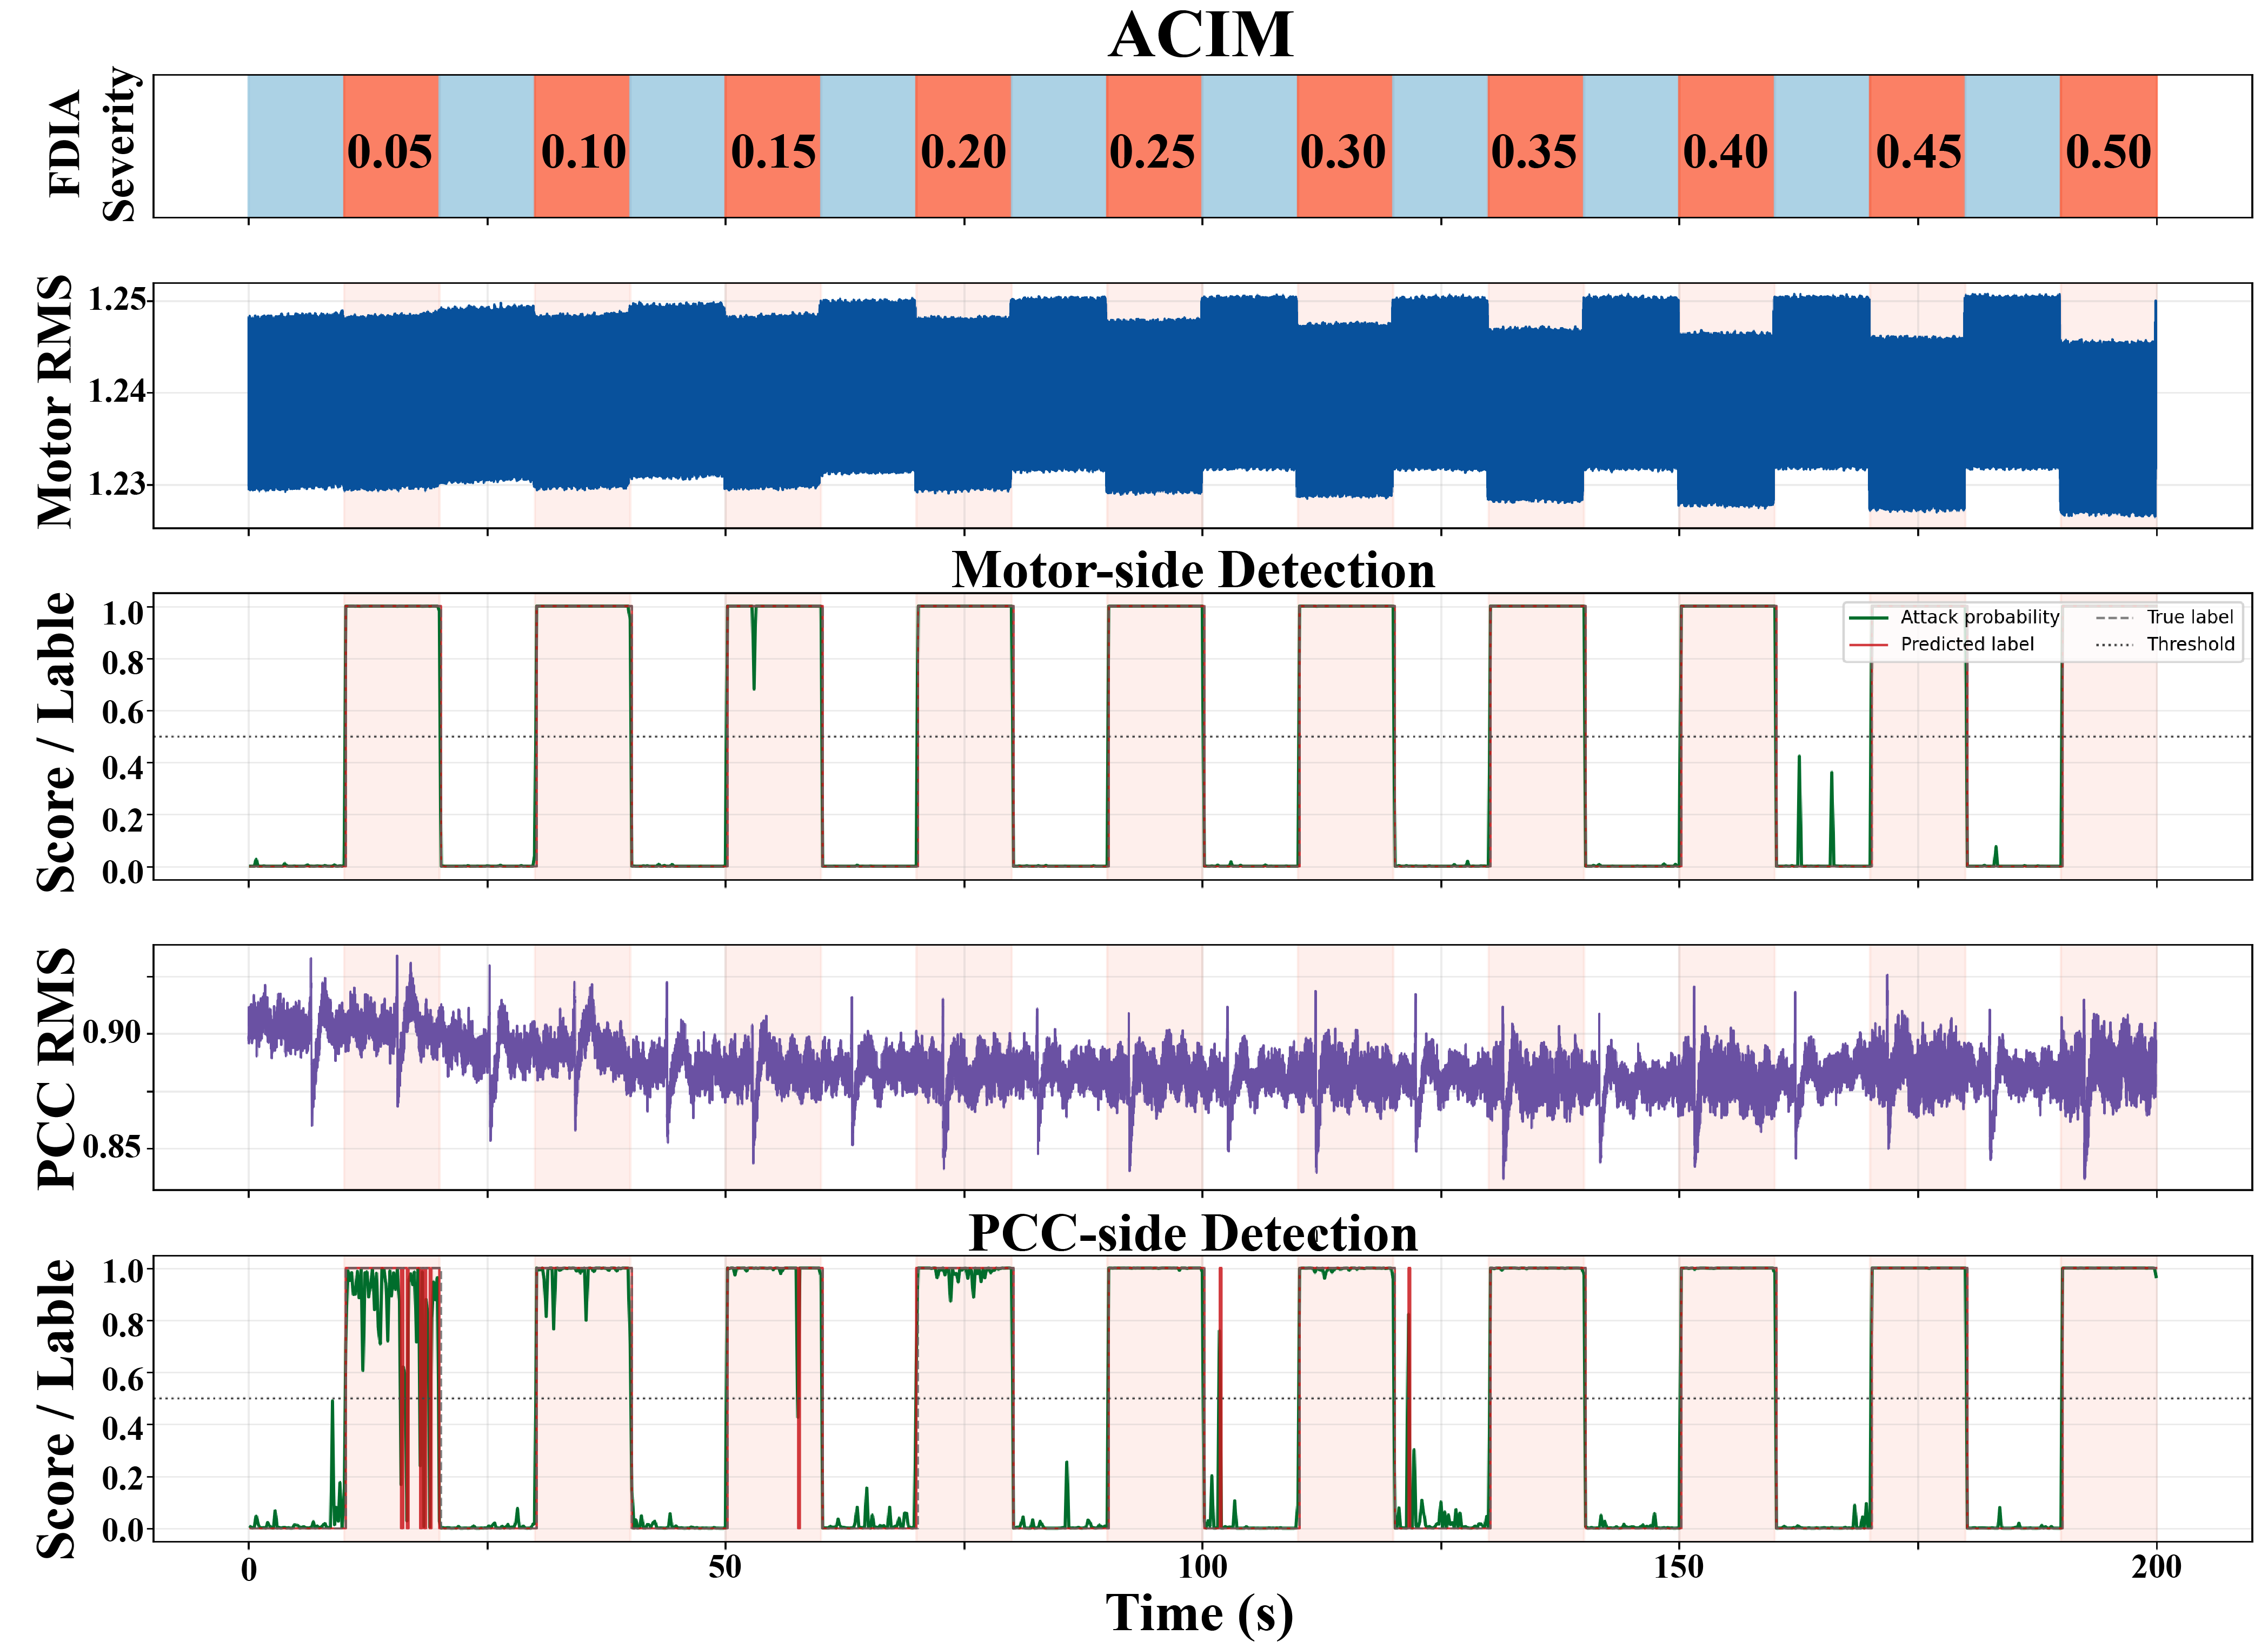
\includegraphics[width=0.98\columnwidth]{figs/case1_30_motor_pcc_model_detection_200s_0p2s_rms61_continuous_revised.png}
    {}
    \vspace{0.3em}
    \textbf{(a)} 200 s overview

    \vspace{0.8em}

    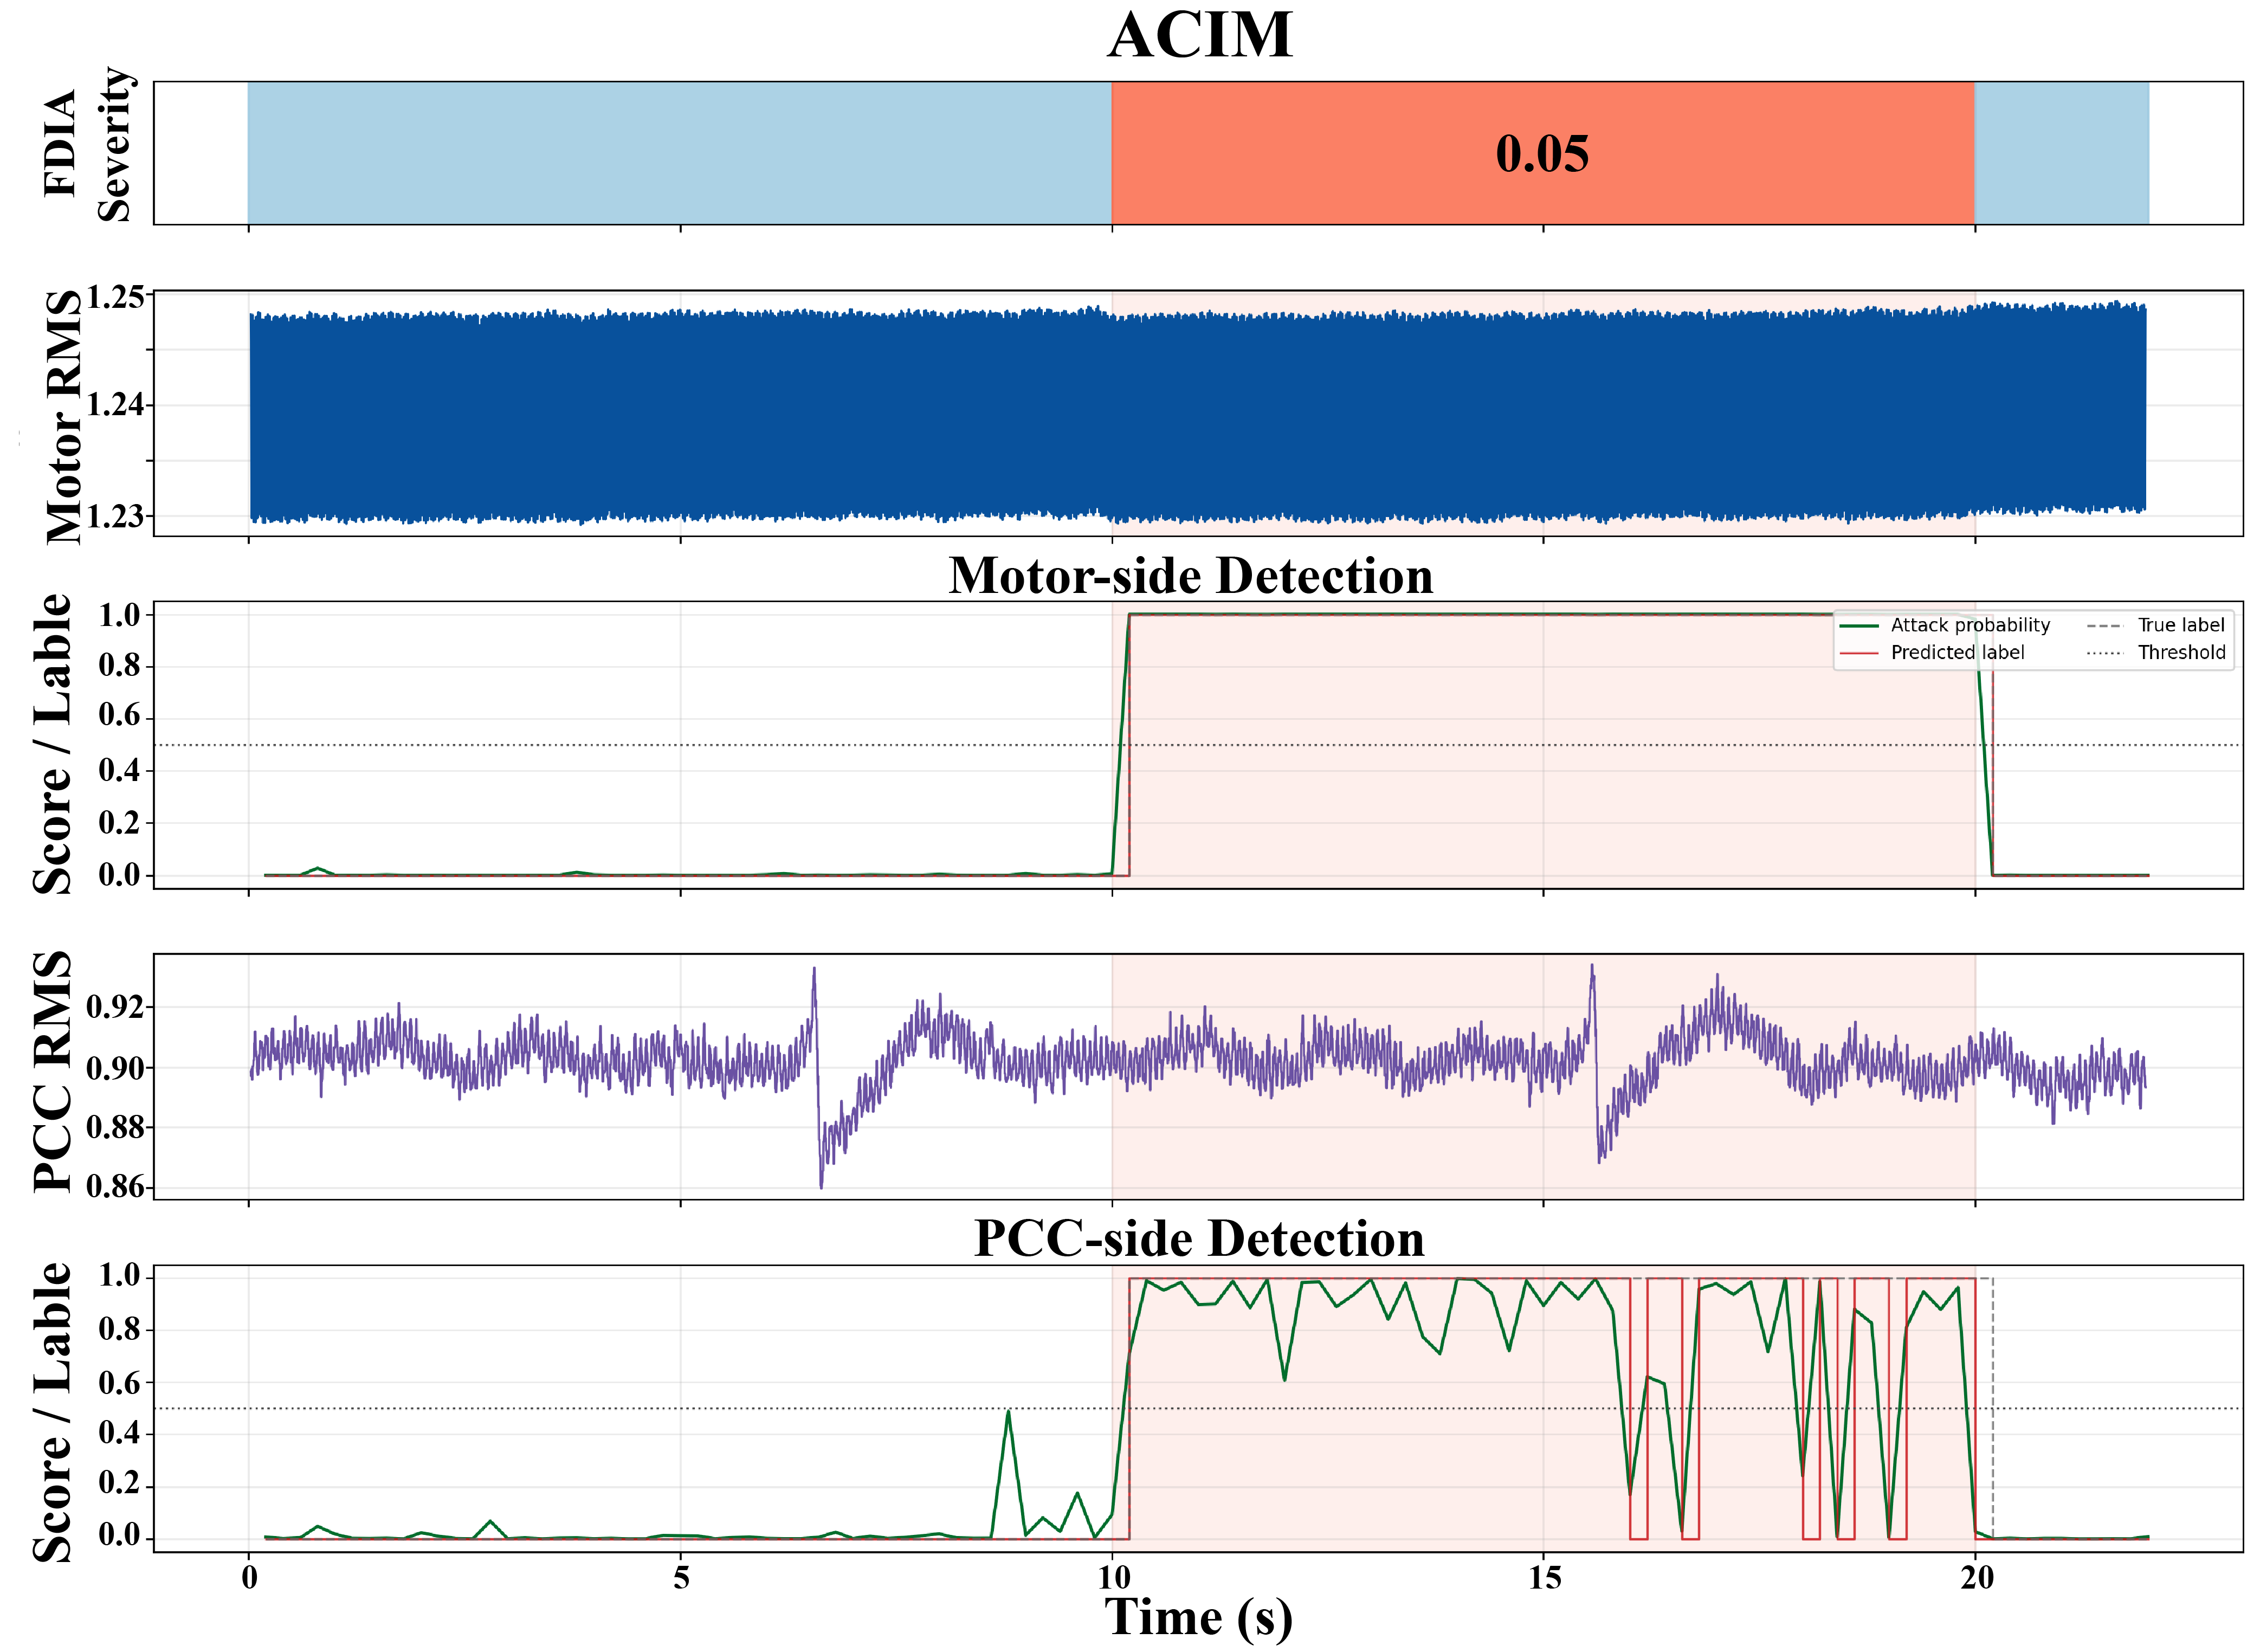
\includegraphics[width=0.98\columnwidth]{figs/case1_30_motor_pcc_model_detection_0_22s_0p2s_rms61_continuous_revised.png}
    
    \vspace{0.3em}
    \textbf{(b)} 0--22 s zoomed view
    \caption{Representative continuous-signal FDIA detection example for the ACIM. Panel (a) shows the 200-s sequence, and panel (b) zooms into the minor attack transition.}
    \label{fig:case1_30_motor_pcc_detection_examples}
\end{figure}


\section{LATENCY AND REDUCED-FEATURE INFERENCE ANALYSIS}
\label{sec:realtime}
Practical PCC monitoring requires low latency and stable online throughput. This section reports per-window latency, throughput, pruning, and reduced-feature effects. In particular, the analysis focuses on end-to-end processing latency, online throughput, feature-pruning effects, and practical considerations for deployment at the PCC. 

\subsection{Inference Latency and Throughput on CPU/GPU}
\label{sec:latency_throughput}
Runtime was benchmarked on an Intel Core Ultra 9 285K CPU and NVIDIA RTX 5090 GPU using the selected LF/HF-Inception pipelines. The benchmark was split into three stages: (i) LF/HF feature extraction from one 2{,}000-sample raw window, (ii) model inference on the resulting feature tensor, and (iii) end-to-end per-window execution. GPU inference was measured with and without host-to-device transfer.

Table~\ref{tab:runtime_latency} summarizes the measured per-window latencies. For the PCC stream, LF/HF feature extraction required 21.72~ms on CPU and the Inception model needs only 0.71~ms on GPU. When host-to-device transfer was included, the GPU inference stage remained sub-millisecond at 0.74~ms. As a result, the PCC end-to-end latency was only 22.46~ms for End-to-End inference.
A similar pattern was observed for the motor stream. Feature extraction required 65.25~ms on CPU, while model inference required 0.36~ms on GPU. Including transfer, the GPU inference stage was 0.38~ms, leading to an end-to-end latency of 65.63~ms. For the tested PCC pipeline, the measured end-to-end latency was 22.46 ms under the reported hardware configuration. In terms of throughput, the end-to-end PCC pipeline sustained 44.53 windows/s, while the corresponding motor pipeline sustained 15.24 windows/s. 

\begin{table}[t]
\centering
\scriptsize
\caption{Measured per-window latency and throughput of the GPU-assisted LF/HF-InceptionTime pipeline.}
\label{tab:runtime_latency}
\renewcommand{\arraystretch}{1.15}
\setlength{\tabcolsep}{3pt}
\begin{tabular}{l c c c c c}
\hline
Stream & Feature & GPU Inference & GPU Transfer + & End-to-End & Throughput \\
 & Extraction (ms) & (ms) & Inference (ms) & (ms) & (windows/s) \\
\hline
PCC   & 21.72 & 0.71 & 0.74 & 22.46 & 44.53 \\
Motor & 65.25 & 0.36 & 0.38 & 65.63 & 15.24 \\
\hline
\end{tabular}
\end{table}

\subsection{Feature Pruning for Low-Latency Anomaly Detection}
\label{sec:latency_throughput}
Feature pruning was evaluated for the \texttt{fdia2} task to reduce online latency. Features were ranked by permutation importance, defined as the balanced-accuracy drop caused by permuting each feature column. Reduced subsets were then formed using global top-\(75\%\), top-\(50\%\), and top-\(25\%\) rankings, as well as per-channel top-15 and top-10 selections. Because the benchmark uses selective LF/HF feature computation, only retained features are extracted; therefore, the measured extraction latency reflects the computational benefit of pruning.


Table~\ref{tab:feature_pruning_anomaly2_runtime} shows that pruning can reduce latency while preserving, and in some cases improving, detection performance. For the PCC stream, the best tradeoff was obtained with the top-\(25\%\) subset, which retained 18 of 74 features. This subset improved balanced accuracy from 88.99\% to 90.11\% and reduced end-to-end CPU+GPU latency from 25.38~ms to 19.71~ms, corresponding to a 1.29\(\times\) speedup. For the motor stream, the top-\(25\%\) subset retained 56 of 222 features, improved balanced accuracy from 98.85\% to 99.48\%, and reduced latency from 109.07~ms to 56.21~ms, corresponding to a 1.94\(\times\) speedup.

The intermediate subsets did not always reduce runtime, even when they contained fewer features. This indicates that pruning effectiveness depends not only on feature count, but also on which LF, HF, and TD feature families remain active. The feature-importance rankings in Fig.~\ref{fig:top10_feature_importance} further show that the two sensing streams rely on different features: motor-side detection is dominated by TD and selected LF features, whereas PCC-side detection places greater emphasis on harmonic and waveform-shape features.
\begin{figure*}[t]
    \centering
    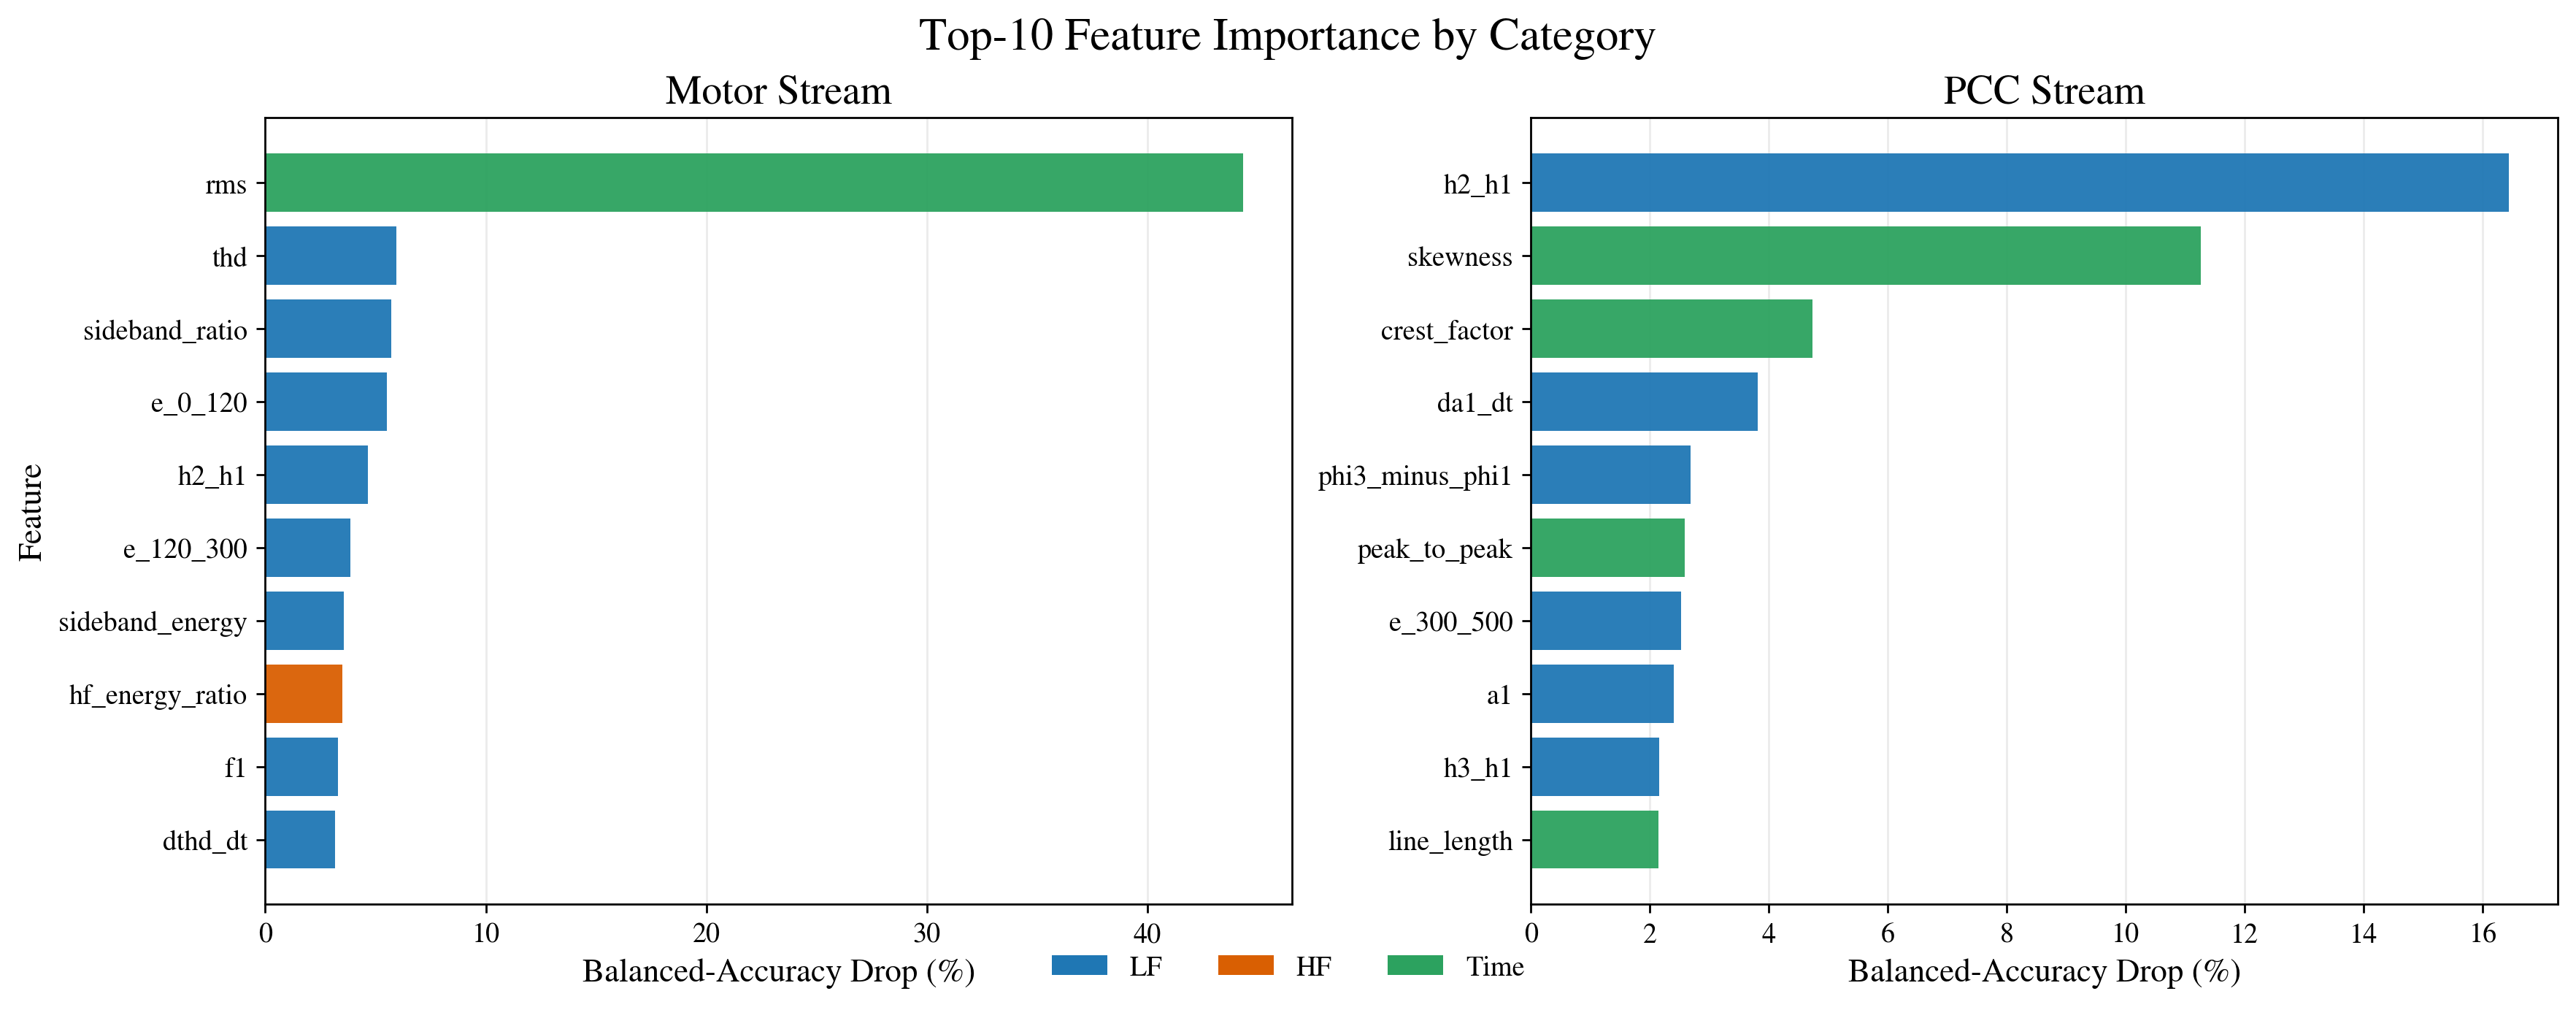
\includegraphics[width=0.95\textwidth]{figs/top10_feature_importance_motor_pcc_typed_clean.png}
    \caption{Feature-importance rankings for the motor and PCC streams.}
    \label{fig:top10_feature_importance}
\end{figure*}

Overall, the LF/HF representation contains redundancy for anomaly detection, and structured pruning can improve both latency and predictive performance. This is especially relevant for PCC-based monitoring, where the compact top-\(25\%\) subset provides both the fastest and most accurate PCC detector.

\begin{table}[t]
\centering
\scriptsize
\caption{Effect of feature pruning on \texttt{fdia2} performance and runtime.}
\label{tab:feature_pruning_anomaly2_runtime}
\renewcommand{\arraystretch}{1.05}
\setlength{\tabcolsep}{2.5pt}
\begin{tabular}{l c c c c c c c}
\hline
Feature & No. & Balanced & F1 & Feature & End-to-End & Speedup & Runtime \\
Set & Feature & Accuracy (\%) & (\%) & Extraction (\%) & (ms) & ($\times$) & Gain(\%) \\
\hline
\multicolumn{7}{c}{\textit{PCC stream}} \\
\hline
Full   & 74  & 88.99 & 89.25 & 24.61 & 25.38  & 1.00 & 0 \\
75\%   & 56  & 88.65 & 88.88 & 22.11 & 22.91 & 1.11 & 11 \\
50\%   & 37  & 88.90 & 89.04 & 22.26 & 23.00 & 1.10 & 10 \\
25\%   & 18  & 90.11 & 90.28 & 18.88 & 19.71 & 1.29 & 29 \\
15/ch. & 30  & 89.33 & 89.52 & 33.95 & 34.70 & 0.73 & -27 \\
10/ch. & 20  & 89.40 & 89.61 & 19.09 & 20.23 & 1.25 & 25 \\
\hline
\multicolumn{7}{c}{\textit{Motor stream}} \\
\hline
Full   & 222 & 98.85 & 98.88 & 108.65 & 109.07 & 1.00 & 0 \\
75\%   & 166 & 99.24 & 99.27 & 110.15 & 110.74 & 0.98 & -2 \\
50\%   & 111 & 99.39 & 99.38 & 112.59 & 113.20 & 0.96 & -4 \\
25\%   & 56  & 99.48 & 99.51 & 55.84 & 56.21  & 1.94 & 94 \\
15/ch. & 90  & 99.49 & 99.50 & 104.02 & 104.60 & 1.04 & 4 \\
10/ch. & 60  & 99.46 & 99.47 & 62.19 & 62.79  & 1.74 & 74 \\
\hline
\end{tabular}
\end{table}
\subsection{LF/HF/TD Ablation for Binary Anomaly Detection}
\label{sec:lfhf_ablation}
A complementary LF/HF/TD ablation was performed on the \texttt{fdia2} task to identify which feature groups are most useful for binary anomaly detection in the PCC and motor streams. Detailed ablation results are reported in Table~\ref{tab:lfhf_ablation_anomaly2}. For the PCC stream, the LF+Time subset achieved 88.67\% balanced accuracy, close to the full model at 88.99\%, whereas HF-only and HF+Time dropped to 73.98\% and 79.78\%, respectively. For the motor stream, the time-only subset matched or slightly exceeded the full model, reaching 99.45\% balanced accuracy compared with 98.85\% for the full representation, while HF-only dropped to 65.34\%. Overall, the ablation confirms that PCC detection relies mainly on LF+Time information, motor-side detection is driven primarily by TD features, and HF features are the least informative group in both streams. This trend is consistent with the pruning results and supports reduced-feature inference in the tested pipeline.
\begin{table}[t]
\centering
\caption{LF/HF/TD ablation results for \texttt{fdia2}.}
\label{tab:lfhf_ablation_anomaly2}
\renewcommand{\arraystretch}{1.15}
\begin{tabular}{l c c c c}
\hline
Feature & Selected & Accuracy & Balanced & F1 (\%) \\
Group & Features & (\%) & Accuracy (\%) & \\
\hline
\multicolumn{5}{c}{\textit{PCC stream}} \\
\hline
Full & 74  & 89.44 & 88.99 & 89.25 \\
LF only   & 36  & 88.31 & 87.89 & 88.11 \\
HF only   & 22  & 74.43 & 73.98 & 74.06 \\
Time only & 16  & 80.48 & 79.71 & 79.99 \\
LF + HF   & 58  & 84.04 & 83.66 & 83.80 \\
LF + Time & 52  & 89.22 & 88.67 & 88.99 \\
HF + Time & 38  & 80.19 & 79.78 & 79.89 \\
\hline
\multicolumn{5}{c}{\textit{Motor stream}} \\
\hline
Full      & 222 & 98.89 & 98.85 & 98.88 \\
LF only   & 108 & 89.77 & 89.48 & 89.62 \\
HF only   & 66  & 66.06 & 65.34 & 65.41 \\
Time only & 48  & 99.47 & 99.45 & 99.46 \\
LF + HF   & 174 & 88.98 & 88.63 & 88.81 \\
LF + Time & 156 & 99.03 & 99.00 & 99.02 \\
HF + Time & 114 & 99.07 & 99.00 & 99.06 \\
\hline
\end{tabular}
\end{table}


\section{Discussion}
\label{sec:discussion}
\subsection{Why Adaptation Helps More in One Direction}
\label{sec:adaptation_asymmetry}
The adaptation results show that ACIM and PMSM do not form a symmetric transfer pair. PMSM $\rightarrow$ ACIM adaptation is much more effective than ACIM $\rightarrow$ PMSM adaptation, particularly for PCC sensing. In the PCC stream, the ACIM $\rightarrow$ PMSM model tends to collapse toward the normal class, whereas the PMSM $\rightarrow$ ACIM model retains more attack-sensitive structure and can be corrected with limited labeled ACIM data. Thus, the source motor affects the initial class bias, the retained target-relevant information, and the benefit obtained from few-shot fine-tuning. For practical PCC deployment, a small amount of target-domain calibration data is therefore important when the deployed motor family differs from the source training domain.

\subsection{PCC vs Motor Tradeoffs}
\label{sec:pcc_vs_motor}

The results reveal a consistent tradeoff between sensing convenience and predictive separability. Motor-side measurements provide the clearest attack-sensitive signatures across nearly all tasks. In the in-domain experiments, the motor stream outperformed the PCC stream for both \texttt{fdia2} and \texttt{severity4}, and the confusion matrices showed substantially stronger diagonal structure for motor-side classification. The motor stream also achieved lower regression error in the attack-only severity-regression task, indicating that direct motor-current sensing preserves richer information about attack intensity and progression.

PCC remains the more deployment-oriented option because it avoids direct terminal access and matches shared industrial power infrastructure. Despite lower separability, PCC achieved useful in-domain detection and strong adapted performance, especially for PMSM $\rightarrow$ ACIM transfer.

Overall, the motor stream is the stronger sensing modality when maximum classification performance is the priority, especially for fine-grained severity discrimination. The PCC stream, by contrast, is the more deployment-oriented choice because it avoids invasive sensing while still supporting accurate and computationally efficient FDIA detection. The value of the framework is therefore not in surpassing motor-side sensing, but in improving the accuracy and computational efficiency of PCC-based monitoring on the tested platform.


\subsection{Limitations}
\label{sec:limitations}

Several limitations should be noted when interpreting the present results. First, the study considers only two motor families, ACIM and PMSM, under a fixed experimental FDIA framework. 
Broader validation across additional machines, loads, control modes, sensing setups, and attack families is needed before generalizing beyond the tested platform.

Second, the domain-adaptation analysis is based on supervised few-shot fine-tuning with labeled target-domain data. This does not cover cases where target labels are unavailable or delayed. Unsupervised or self-supervised adaptation strategies may therefore be required for more constrained deployment scenarios.

Third, the deployment analysis was performed using a GPU-assisted software implementation and focused mainly on the binary FDIA detection task; embedded implementation and task-specific optimization for severity assessment remain future work.

Finally, some baselines were competitive under macro-F1; therefore, the conclusions are strongest for accuracy and balanced accuracy, not universal model dominance.
\begin{figure*}[t]
    \centering
    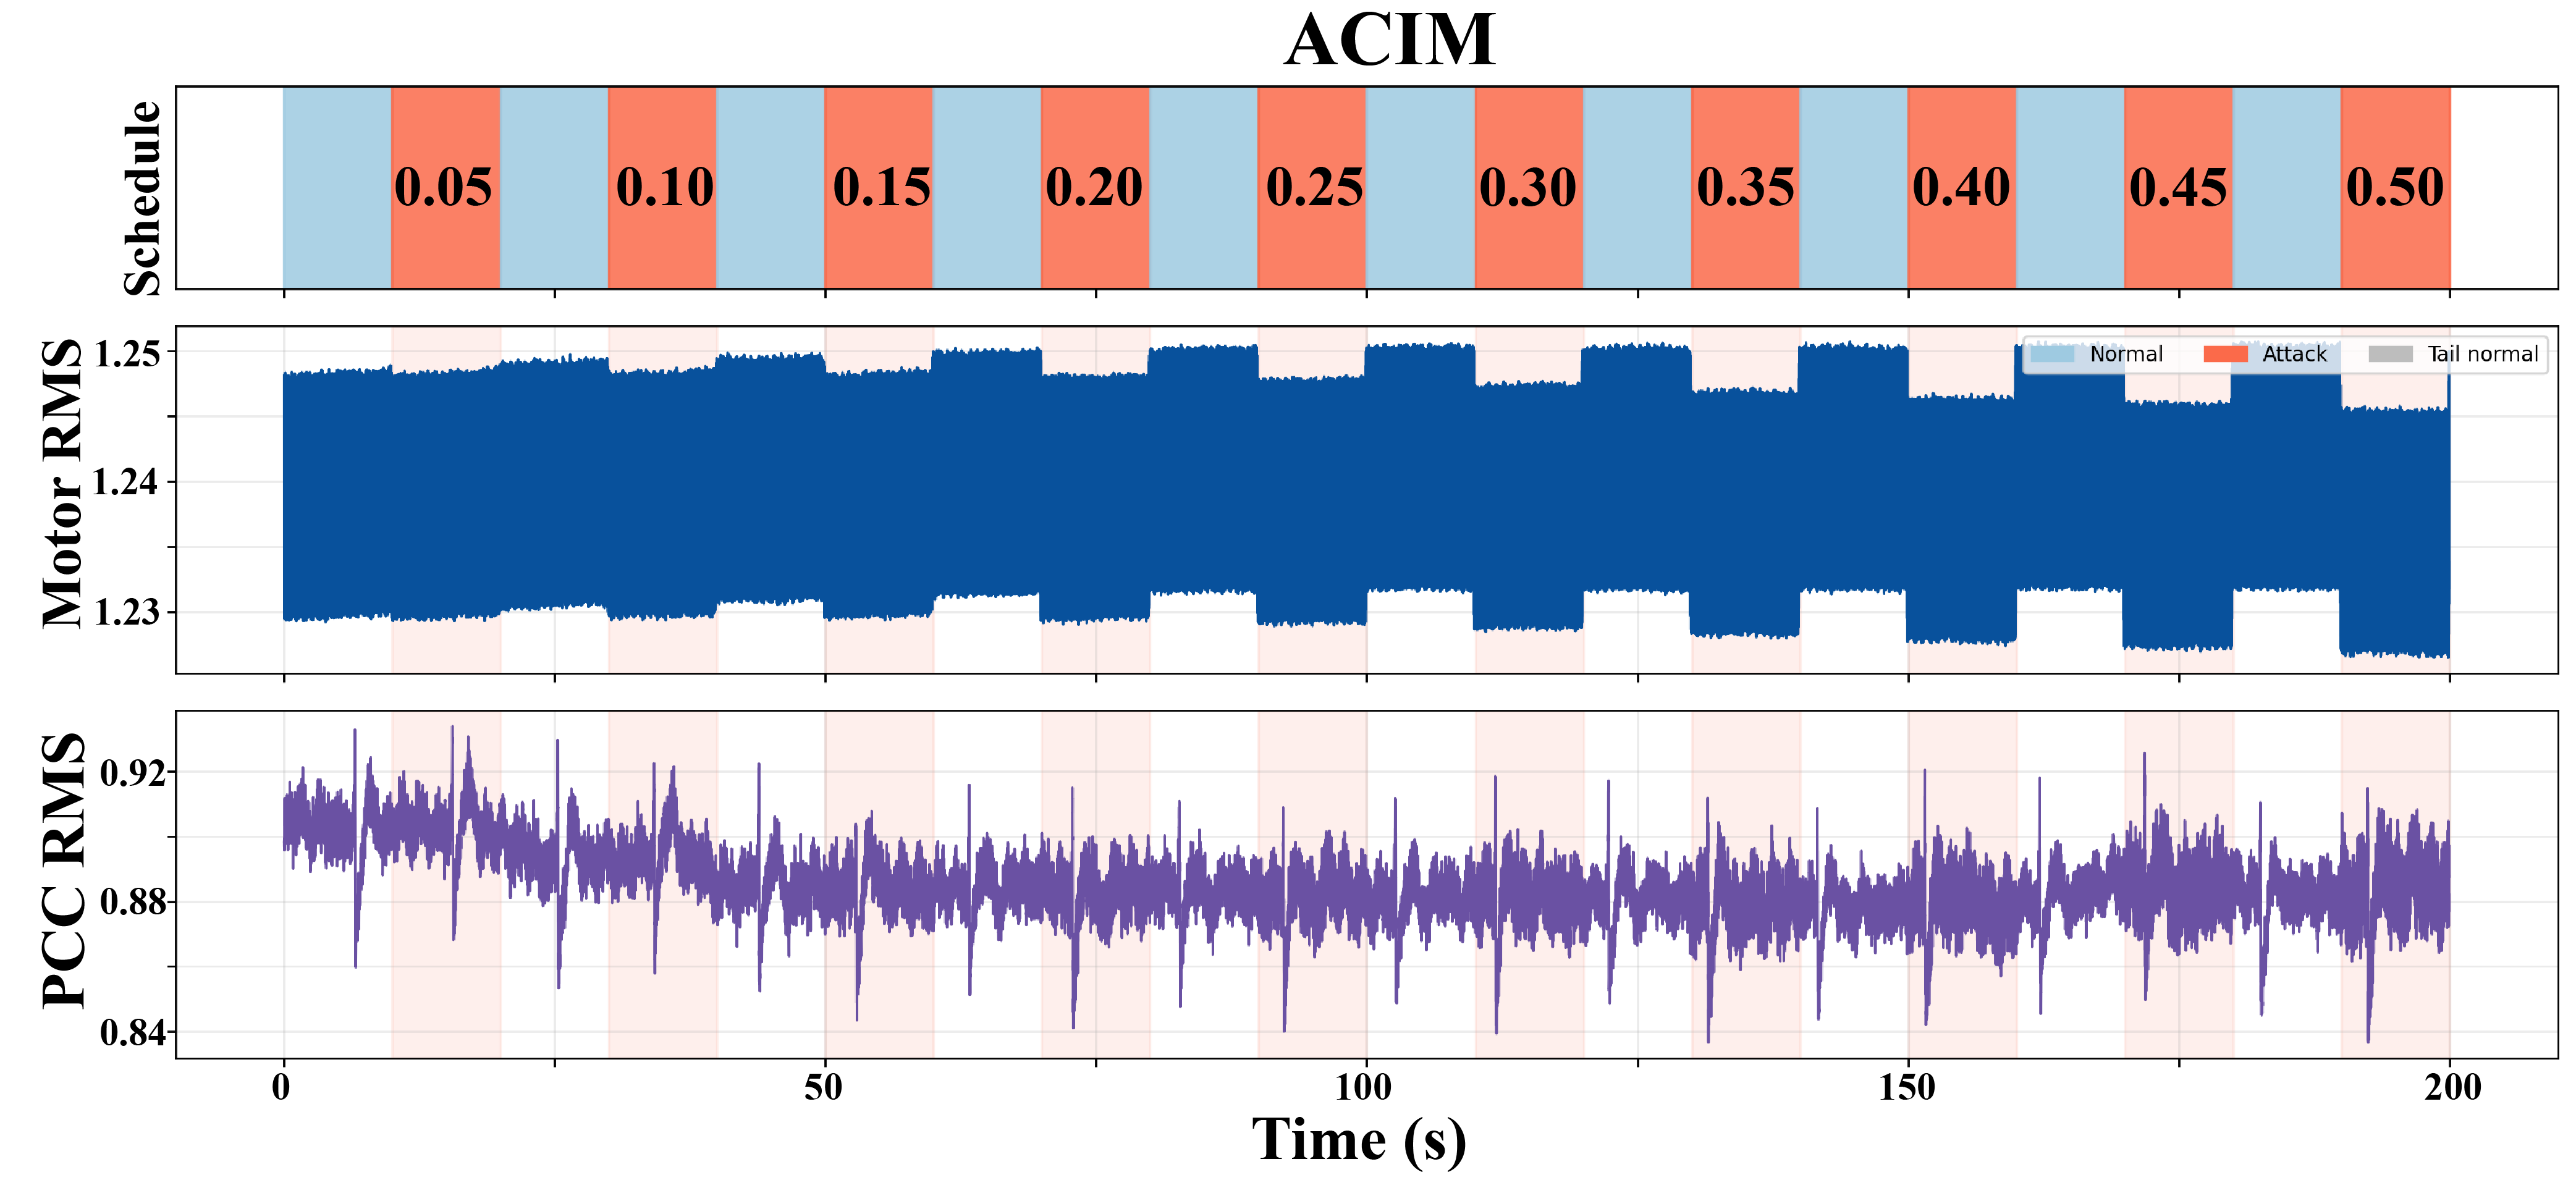
\includegraphics[width=0.49\textwidth]{figs/case1_30_motor_pcc_model_detection_200s_0p2s_rms61_continuous_rows124_revised.png}
    \hfill
    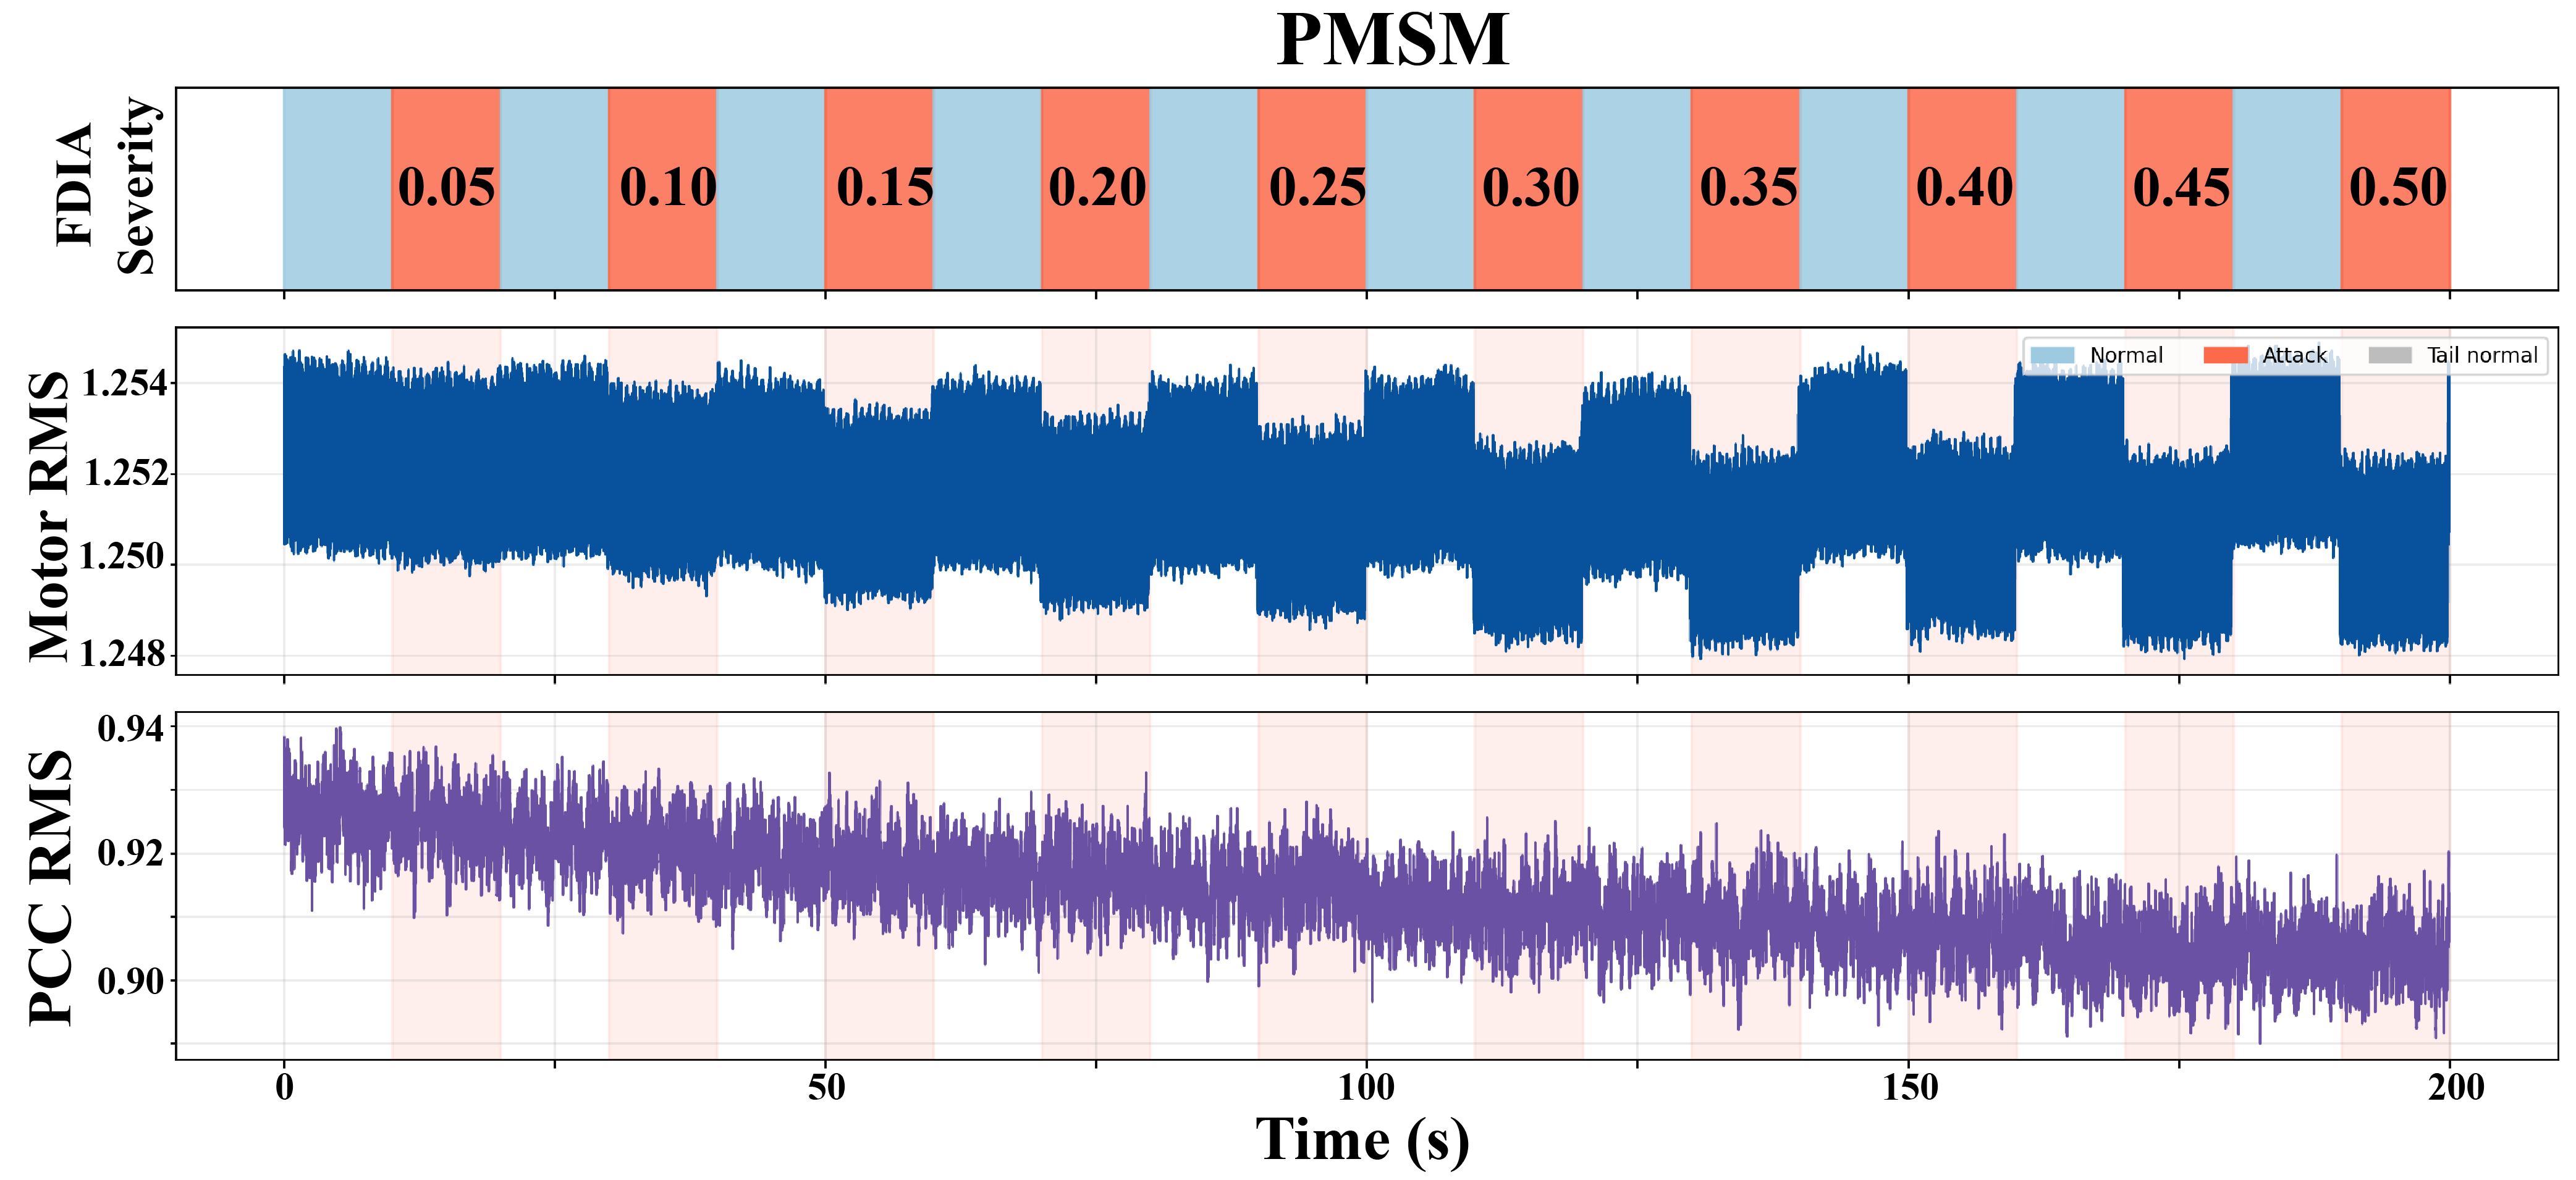
\includegraphics[width=0.49\textwidth]{figs/casepmsm271_300_motor_pcc_model_detection_200s_0p2s_rms61_continuous_rows124_revised.png}
    \caption{Representative consecutive FDIA episodes applied to the ACIM and PMSM motor-drive systems. Top: scheduled FDIA severity; middle: motor-current RMS; bottom: PCC-current RMS.}
    \label{fig:app_attack_process_examples}
\end{figure*}
\section{Conclusion}
\label{sec:conclusion}
This paper experimentally evaluated PCC-based detection of low-severity current-feedback FDIAs in a heterogeneous ACIM/PMSM inverter-fed drive platform. Motor-terminal measurements provided the strongest separability, but PCC measurements supported useful nonintrusive detection despite aggregation, harmonics, and grid-side interactions. In the mixed-domain setting, the proposed LF/HF-InceptionTime method achieved strong \texttt{fdia2} detection from both sensing locations, while PCC \texttt{severity4} estimates were less reliable and should be interpreted as coarse diagnostics. Cross-motor experiments showed substantial ACIM/PMSM domain shift, making source-only transfer unreliable. Few-shot target-domain fine-tuning improved transfer performance, with much larger gains for PMSM $\rightarrow$ ACIM adaptation than for ACIM $\rightarrow$ PMSM adaptation. Runtime and pruning results further indicate that the PCC pipeline is compatible with the required online processing rate. Overall, the results indicate that PCC-based FDIA monitoring is promising on the tested ACIM/PMSM platform under additive current-feedback attacks.

\bibliographystyle{ieeetr}
\bibliography{ref}

\appendices
\section{Additional Experimental and Diagnostic Results}
\label{app:additional_results}

% This appendix provides supplementary experimental and diagnostic material that supports the main results. The additional material includes representative FDIA episodes, the data-acquisition hardware, the extracted LF/HF/TD feature set, motor-type classification diagnostics, and attack-only severity-regression results.

This appendix provides supplementary material supporting the main results, including representative FDIA episodes and the extracted LF/HF/TD feature set.

\subsection{Representative FDIA Episodes}
\label{app:fdia_episode_examples}

Figure~\ref{fig:app_attack_process_examples} shows representative consecutive FDIA episodes applied to the ACIM and PMSM drive systems. In both examples, the top panel shows the scheduled FDIA severity level, while the middle and bottom panels show the corresponding motor-current and PCC-current RMS responses during the first 200~s of operation.


% \subsection{Data-Acquisition Hardware}
% \label{app:data_acquisition_hardware}

% The experimental data were acquired directly from the testbed using a National Instruments cDAQ-9185 chassis and a custom data-collector interface board, as shown in Fig.~\ref{fig:app_data_acquisition_hardware}. The same acquisition setup was used for synchronized motor-side and PCC-side measurements.

% \begin{figure}[t]
%     \centering
%     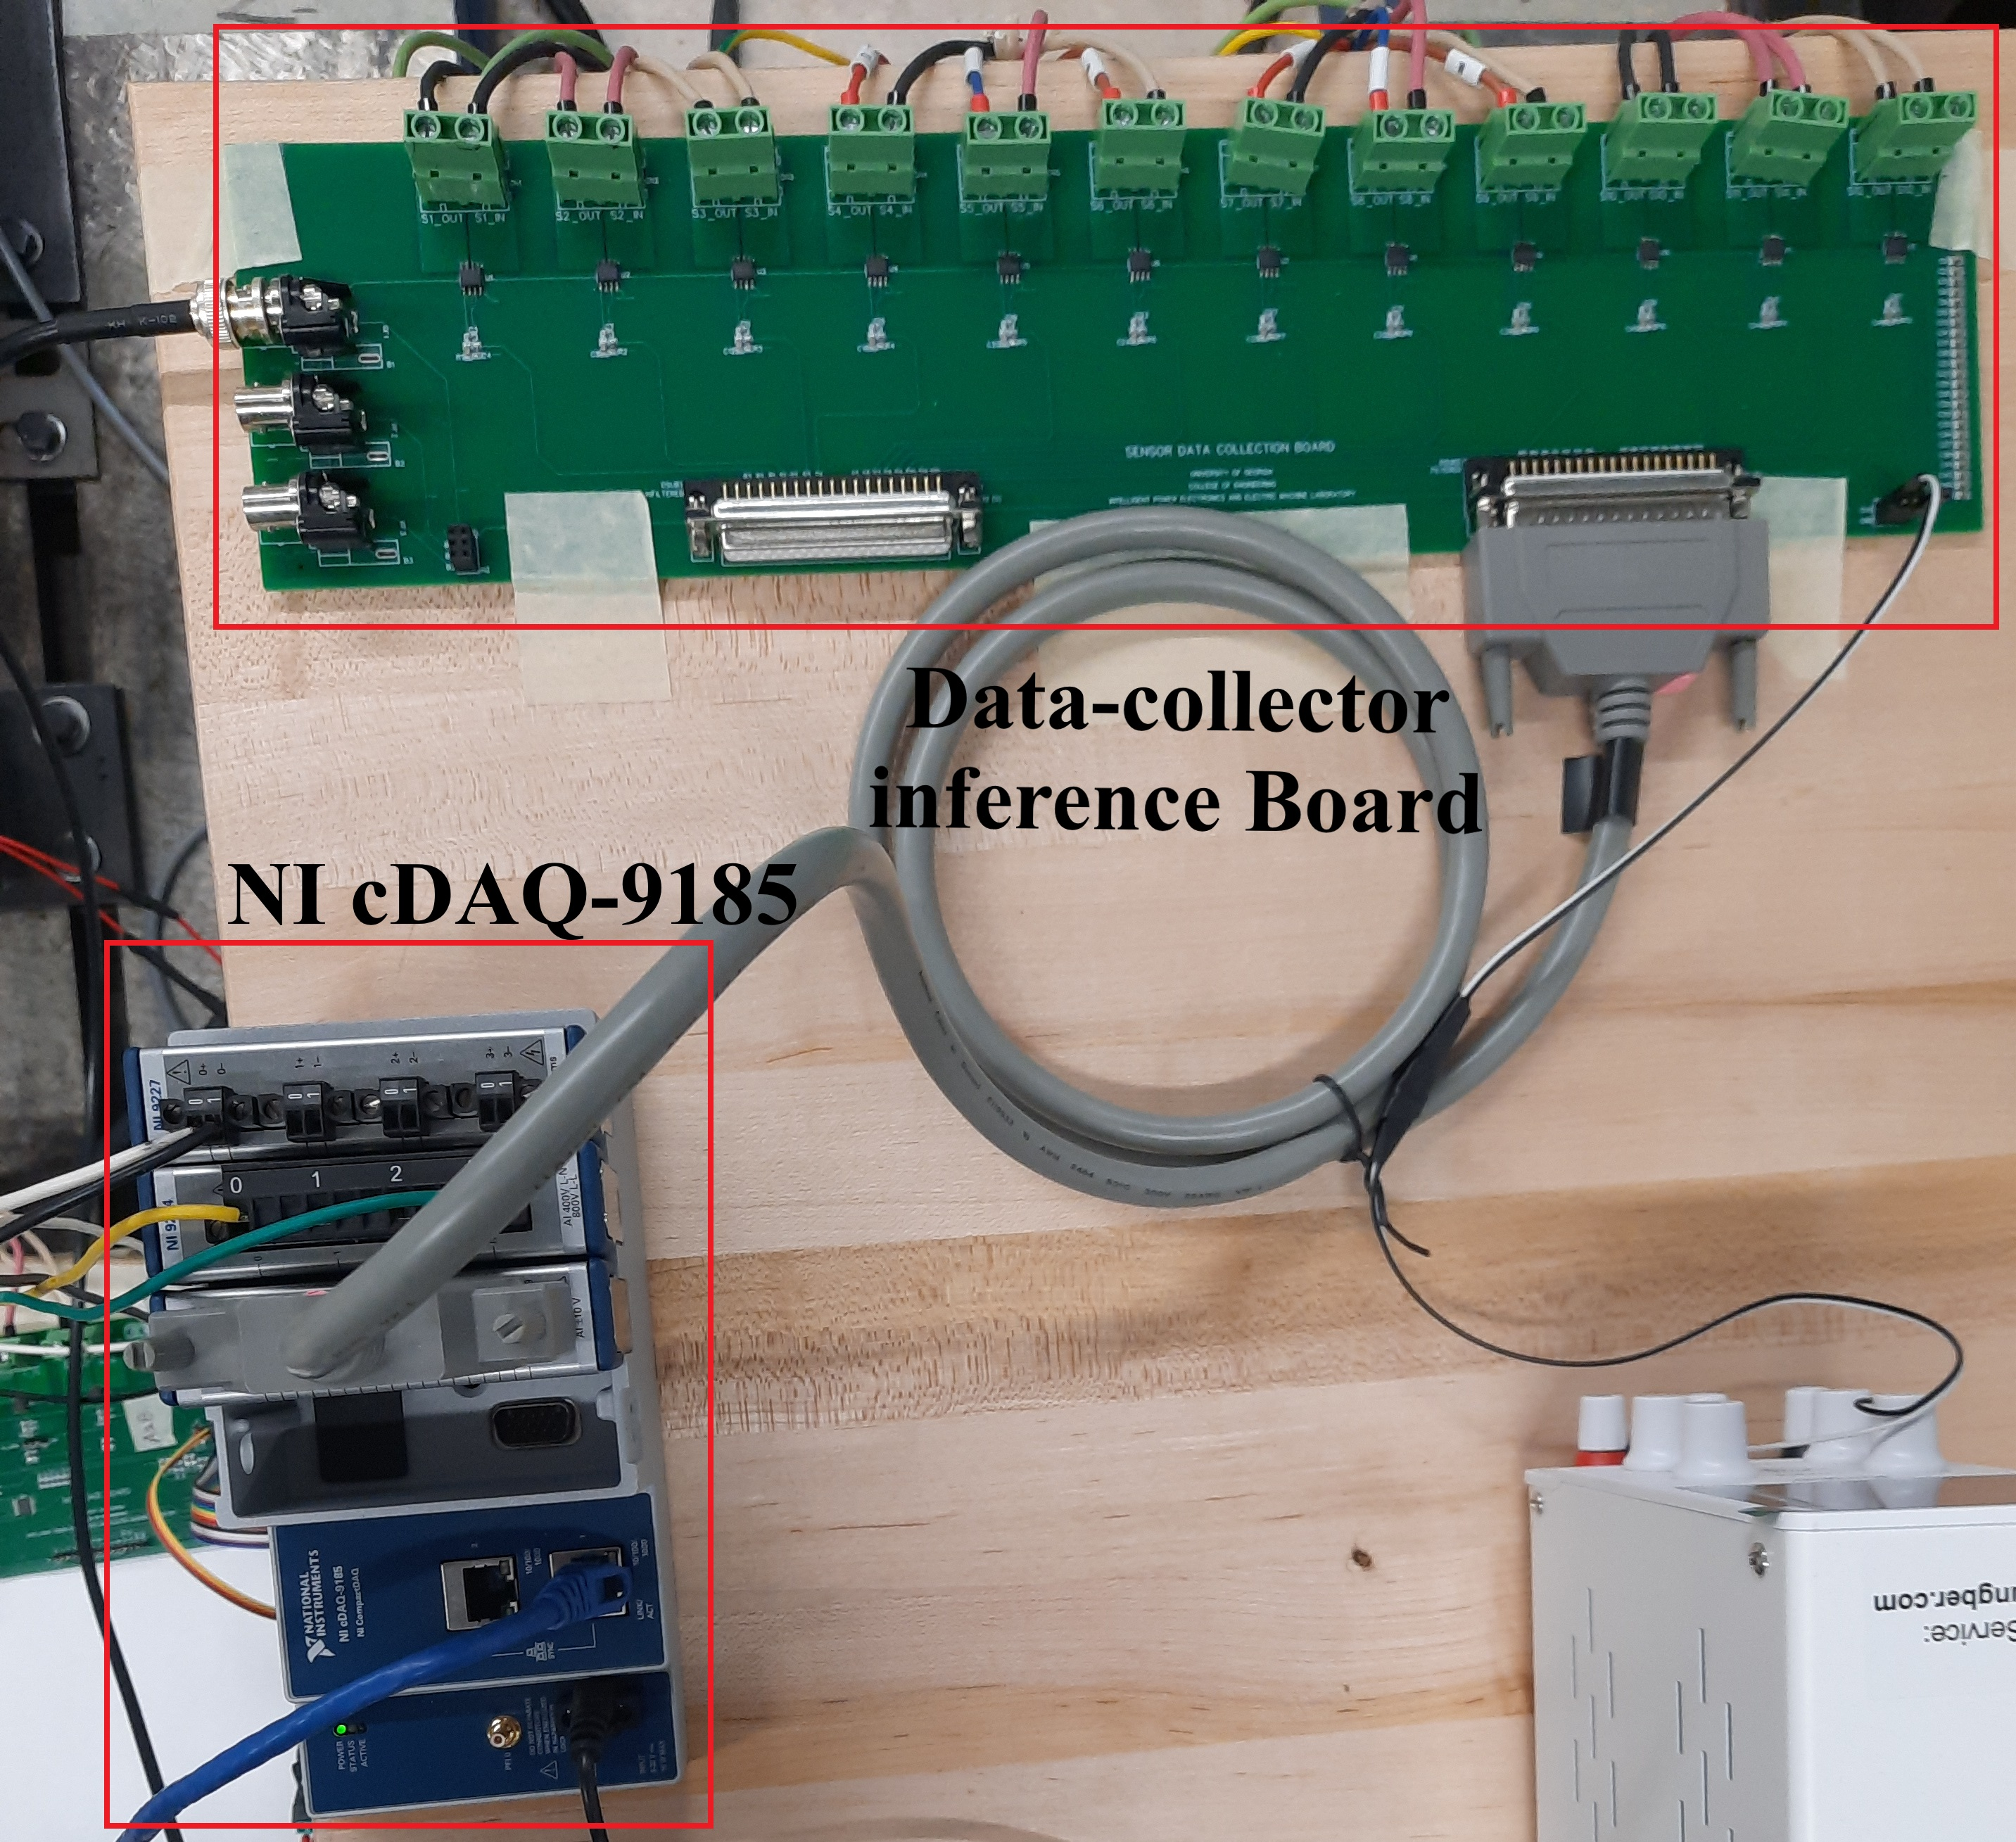
\includegraphics[width=0.70\columnwidth]{figs/data_acquisition_hardware.jpg}
%     \caption{NI cDAQ-9185-based data-acquisition hardware used for synchronized motor-side and PCC-side measurements.}
%     \label{fig:app_data_acquisition_hardware}
% \end{figure}

\subsection{Extracted Feature Set}
\label{app:feature_set}

Table~\ref{tab:app_extracted_features} summarizes the extracted features used in the proposed LF/HF/TD pipeline. Each channel is represented using low-frequency spectral features, high-frequency spectral-envelope features, and time-domain statistical features.

\begin{table}[t]
\centering
\scriptsize
\caption{Extracted features per channel in the proposed LF/HF/TD pipeline.}
\label{tab:app_extracted_features}
\setlength{\tabcolsep}{3pt}
\renewcommand{\arraystretch}{1.08}
\begin{tabularx}{\columnwidth}{l c c X}
\hline
Type & No. & Window / Stride & Features \\
\hline
LF & 18 & 500 / 25 &
$A_1$, $f_1$, $\phi_1$, THD, $H_2/H_1$, $H_3/H_1$, $H_5/H_1$, $H_7/H_1$,
$\phi_3-\phi_1$, $\phi_5-\phi_1$, sideband energy/ratio,
$E_{0-120}$, $E_{120-300}$, $E_{300-500}$,
$df_1/dt$, $dA_1/dt$, $d\mathrm{THD}/dt$ \\
\hline
HF & 11 & 500 / 25 &
RMS$_{2-5k}$, energy ratio, centroid, bandwidth, flatness, kurtosis,
peak frequency, peak-to-band, envelope RMS, envelope kurtosis, envelope crest factor \\
\hline
TD & 8 & 500 / 25 &
RMS, standard deviation, crest factor, kurtosis, skewness, peak-to-peak, line length, Teager MAV \\
\hline
Total & 37 & -- & LF (18), HF (11), TD (8) \\
\hline
\end{tabularx}
\end{table}

% \subsection{Auxiliary Diagnostic Tasks}
% \label{app:auxiliary_diagnostics}

% This subsection reports auxiliary diagnostic results that complement the main classification findings. These diagnostics are not used as the primary performance claims; rather, they provide additional evidence about motor-domain separability and the difficulty of severity estimation from PCC measurements.

% Figure~\ref{fig:app_motor_type_confusion} shows the motor-type classification confusion matrices. Both the motor-side and PCC-side streams exhibit nearly perfect separation between ACIM and PMSM samples. This confirms that the two motor families induce strongly distinguishable electrical domains and supports the domain-adaptation analysis in the main text.

% \begin{figure}[!t]
%     \centering
%     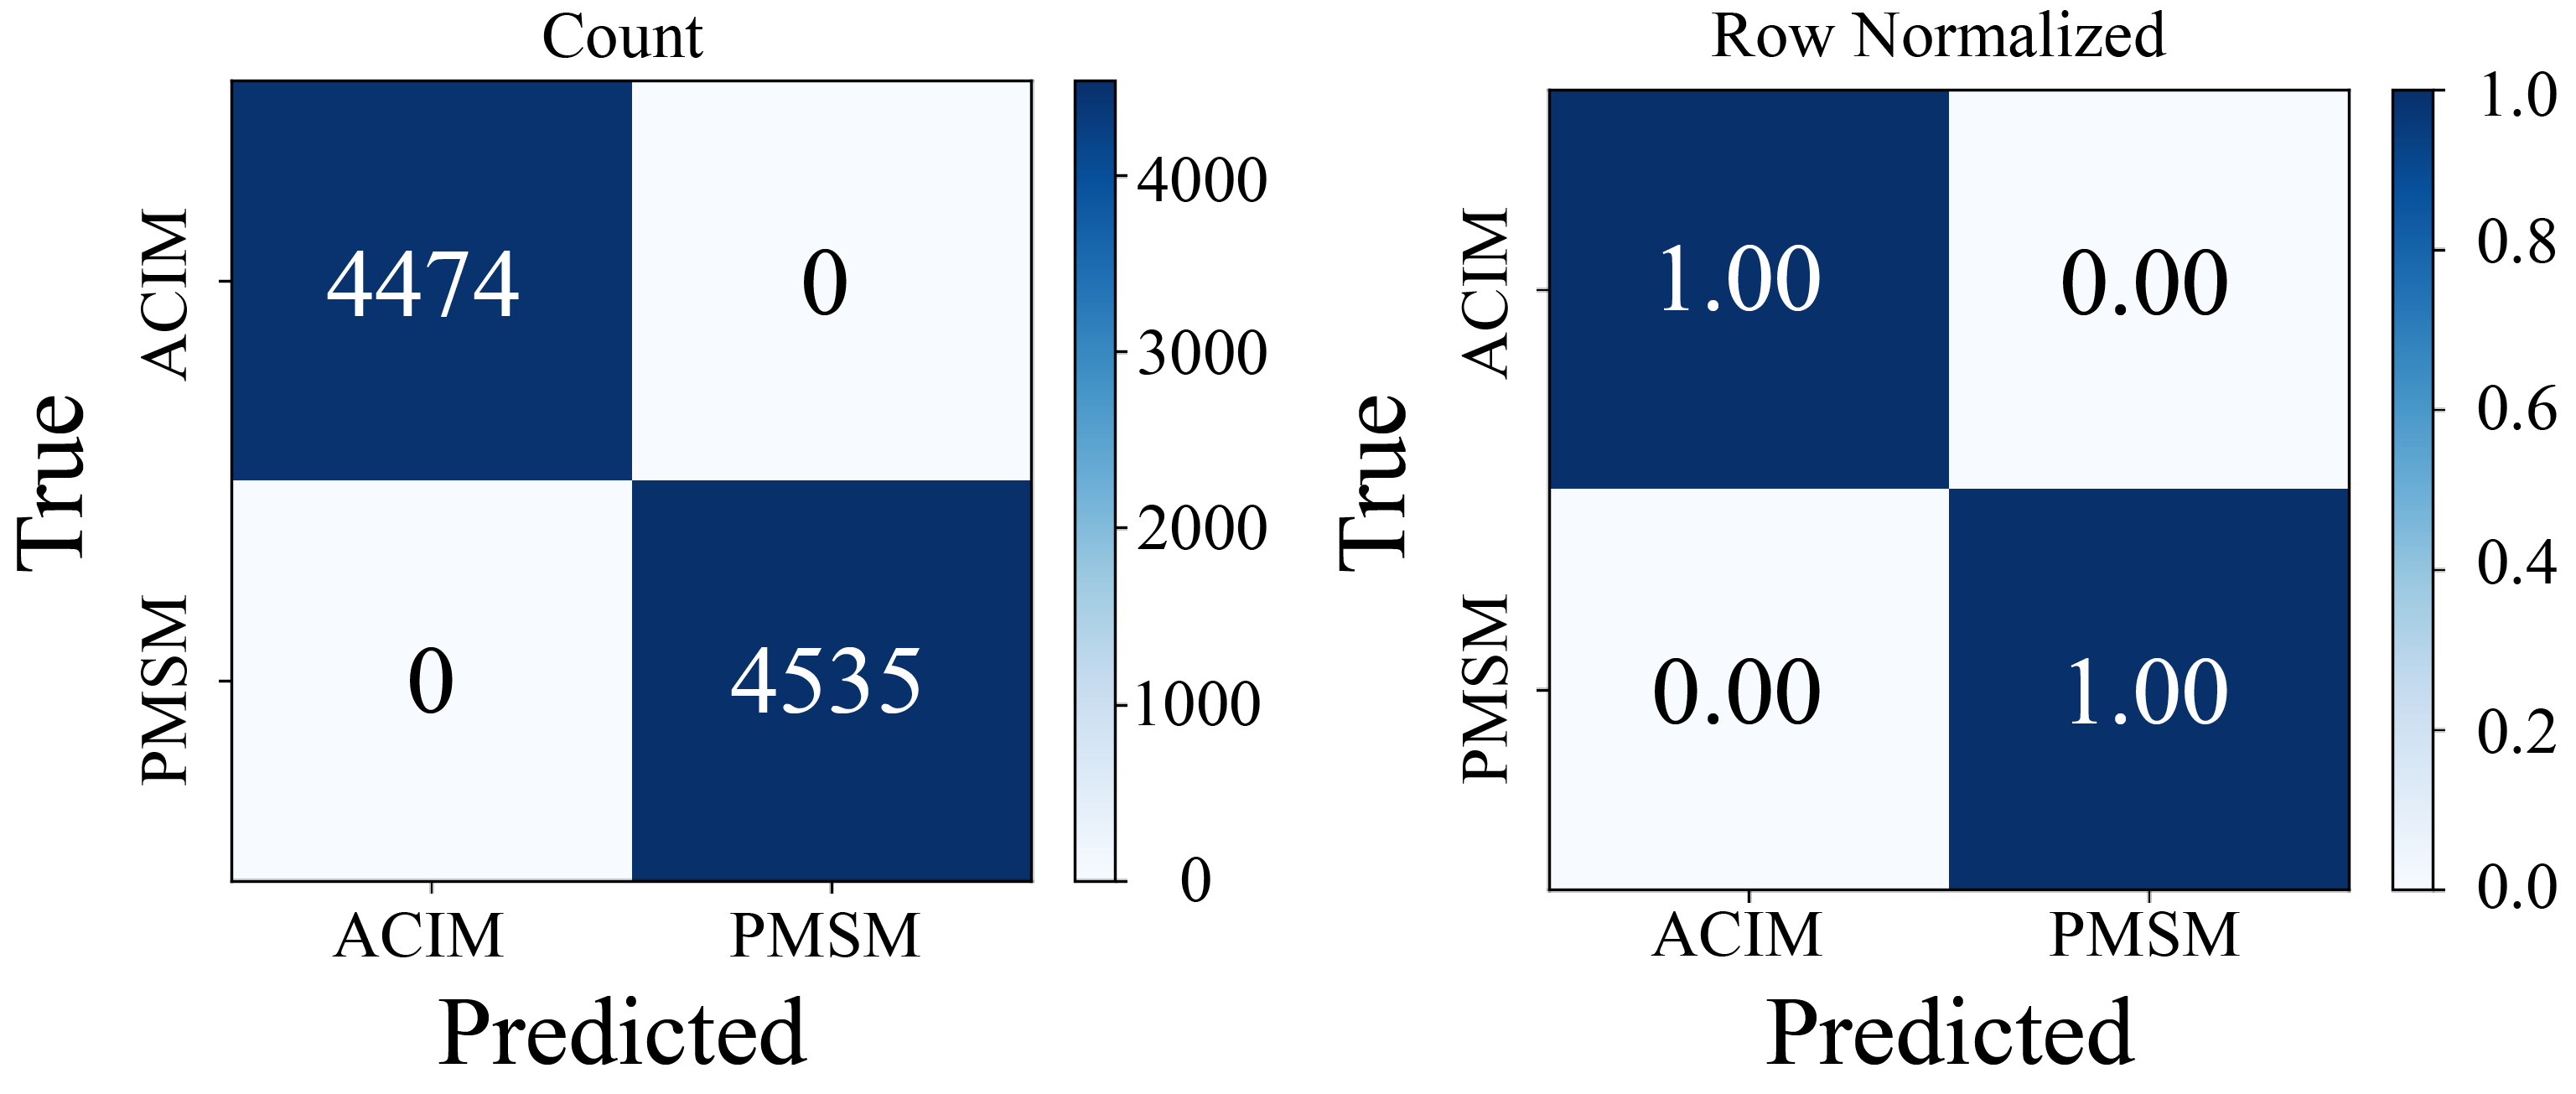
\includegraphics[width=0.98\columnwidth]{figs/motor_type2_motor_confusion_revised.png}

%     \vspace{0.3em}
%     \textbf{(a)} Motor-side stream

%     \vspace{0.8em}

%     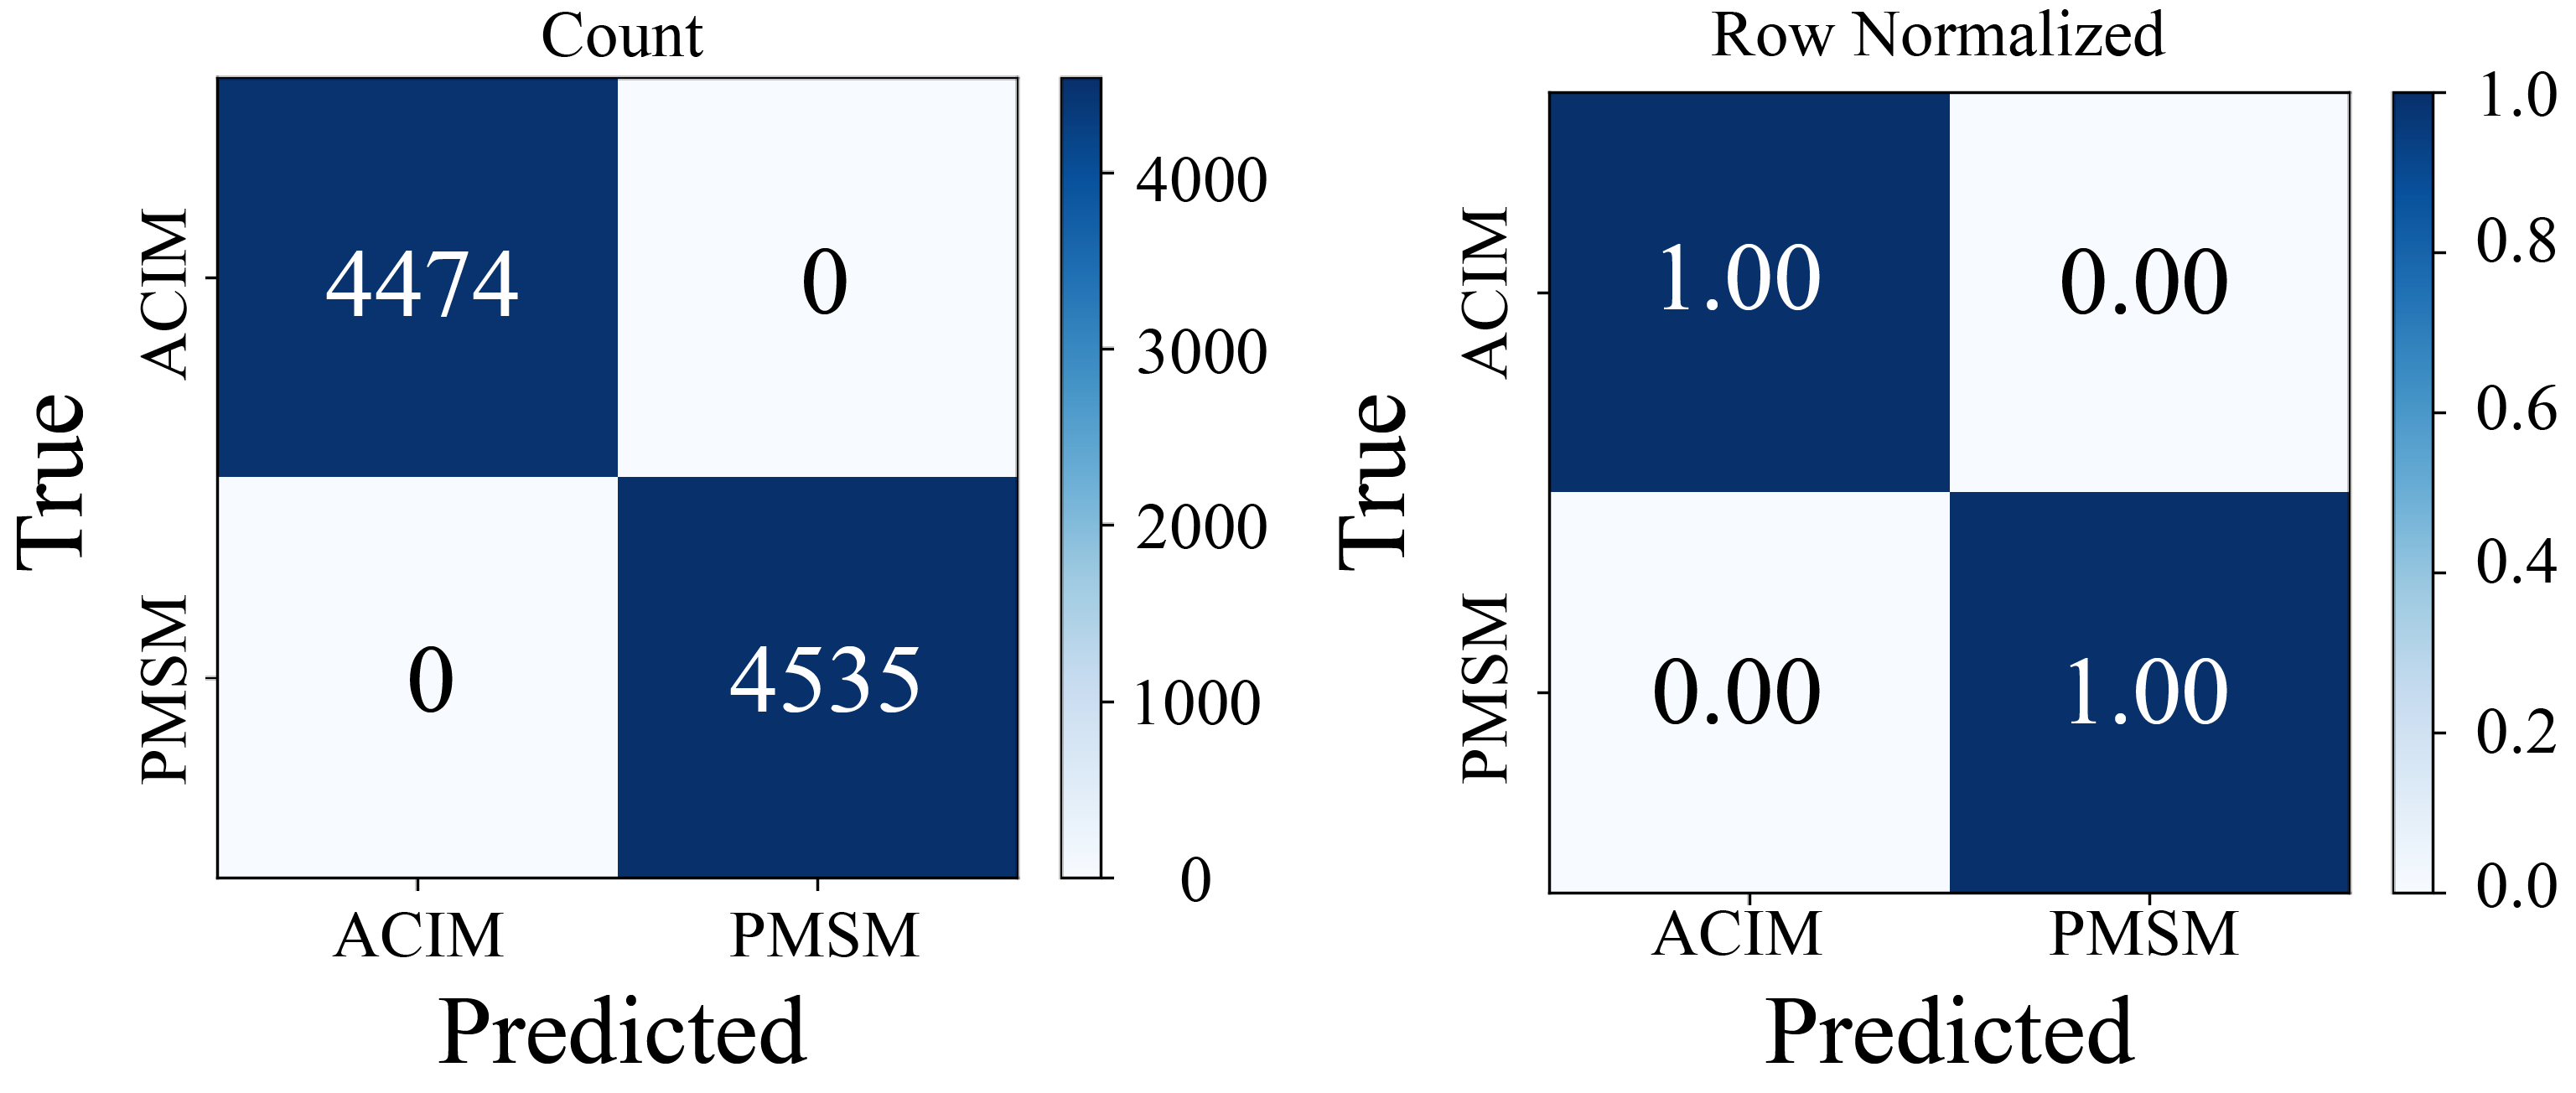
\includegraphics[width=0.98\columnwidth]{figs/motor_type2_pcc_confusion_revised.png}

%     \vspace{0.3em}
%     \textbf{(b)} PCC-side stream

%     \caption{Motor-type classification confusion matrices for the motor-side and PCC-side streams. Panel (a) shows the motor-side results, while panel (b) shows the PCC-side results.}
%     \label{fig:app_motor_type_confusion}
% \end{figure}

% Table~\ref{tab:app_severity_regression} reports the attack-only severity-regression results under the mixed ACIM/PMSM split. The motor-side stream achieves a test MAE of 0.1483 and a test MSE of 0.1818, whereas the PCC-side stream achieves a test MAE of 0.3914 and a test MSE of 0.4226. These results indicate that continuous severity estimation is considerably more reliable from direct motor-side measurements than from PCC-level measurements.

% \begin{table}[t]
% \centering
% \caption{In-domain attack-only severity-regression performance under the mixed ACIM/PMSM split.}
% \label{tab:app_severity_regression}
% \renewcommand{\arraystretch}{1.15}
% \begin{tabular}{l c c}
% \hline
% Stream & Test MAE & Test MSE \\
% \hline
% Motor-side & 0.1483 & 0.1818 \\
% PCC-side   & 0.3914 & 0.4226 \\
% \hline
% \end{tabular}
% \end{table}

% Figure~\ref{fig:app_regression_diagnostics} shows the regression diagnostics for the attack-only severity-regression task. The motor-side parity and residual plots indicate tighter agreement between predicted and true severity values than the corresponding PCC-side results. In the PCC case, the larger residual spread and broader histogram confirm that continuous severity estimation is less reliable at the PCC than from direct motor-side measurements.

% \begin{figure}[!t]
%     \centering
%     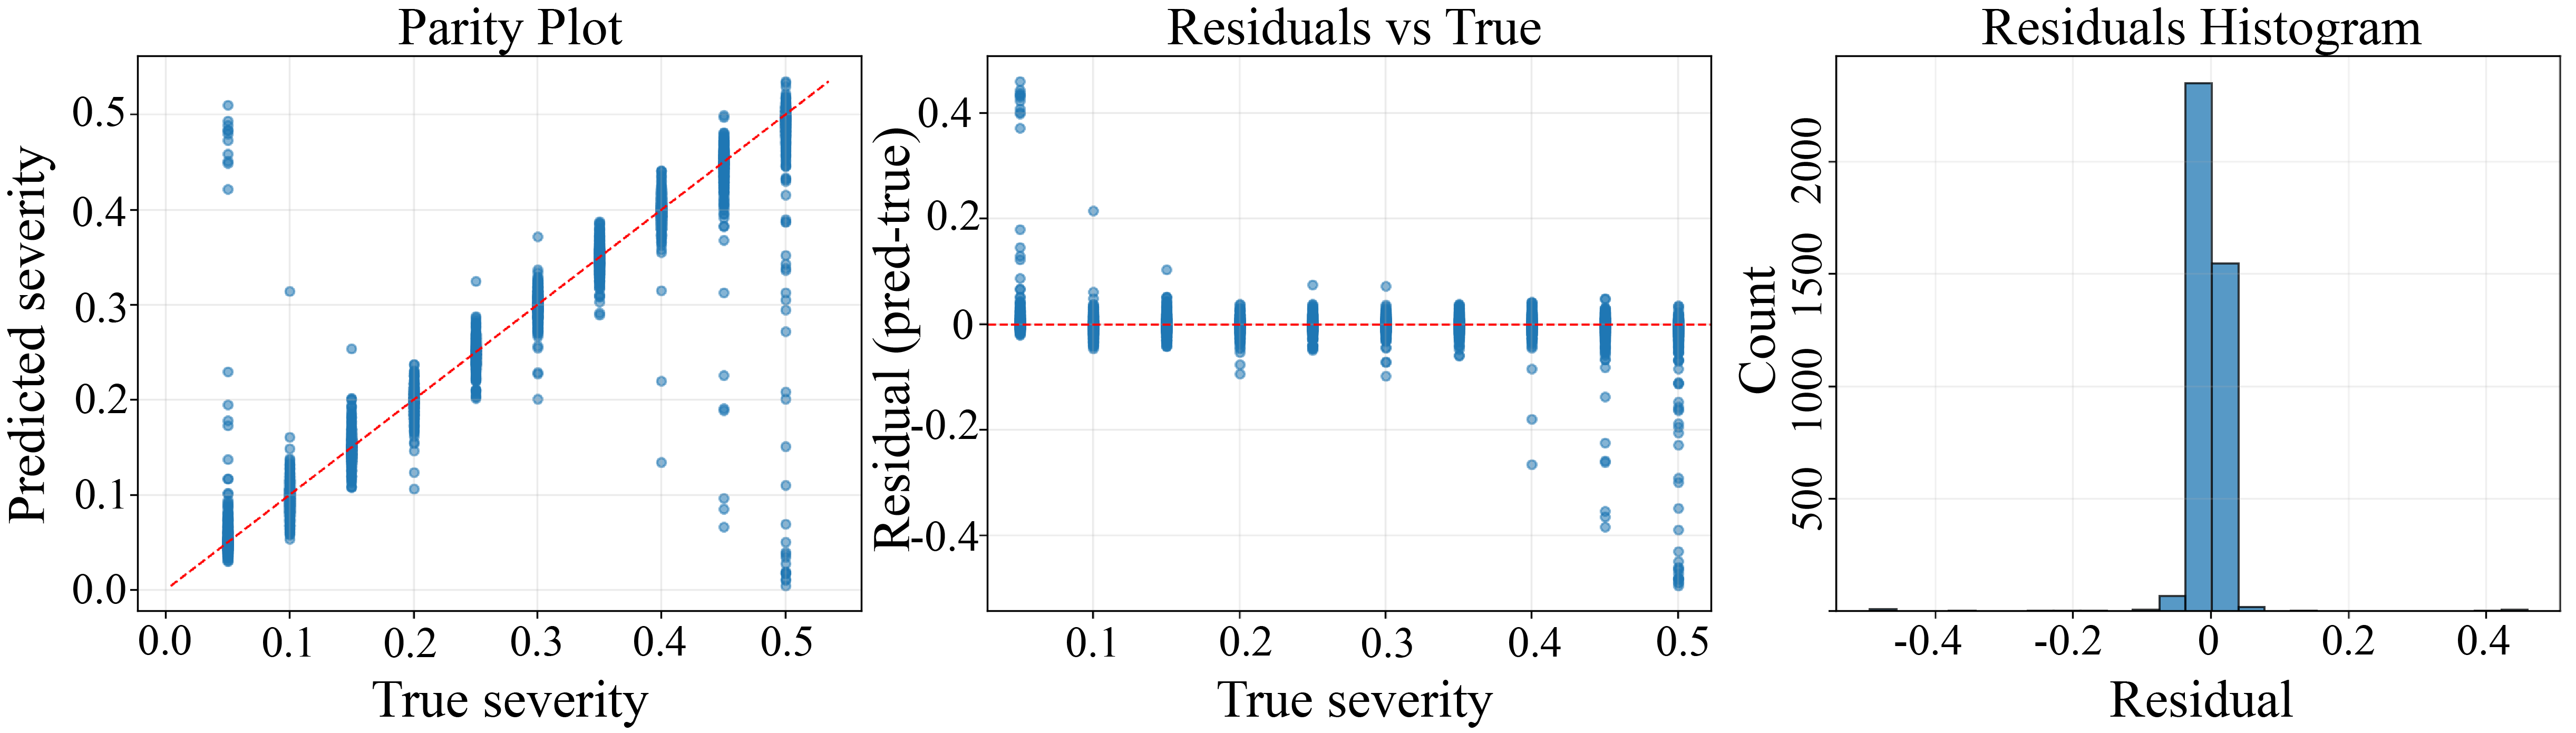
\includegraphics[width=0.98\columnwidth]{figs/severity_reg_attack_motor_diagnostics_revise.png}

%     \vspace{0.3em}
%     \textbf{(a)} Motor-side stream

%     \vspace{0.8em}

%     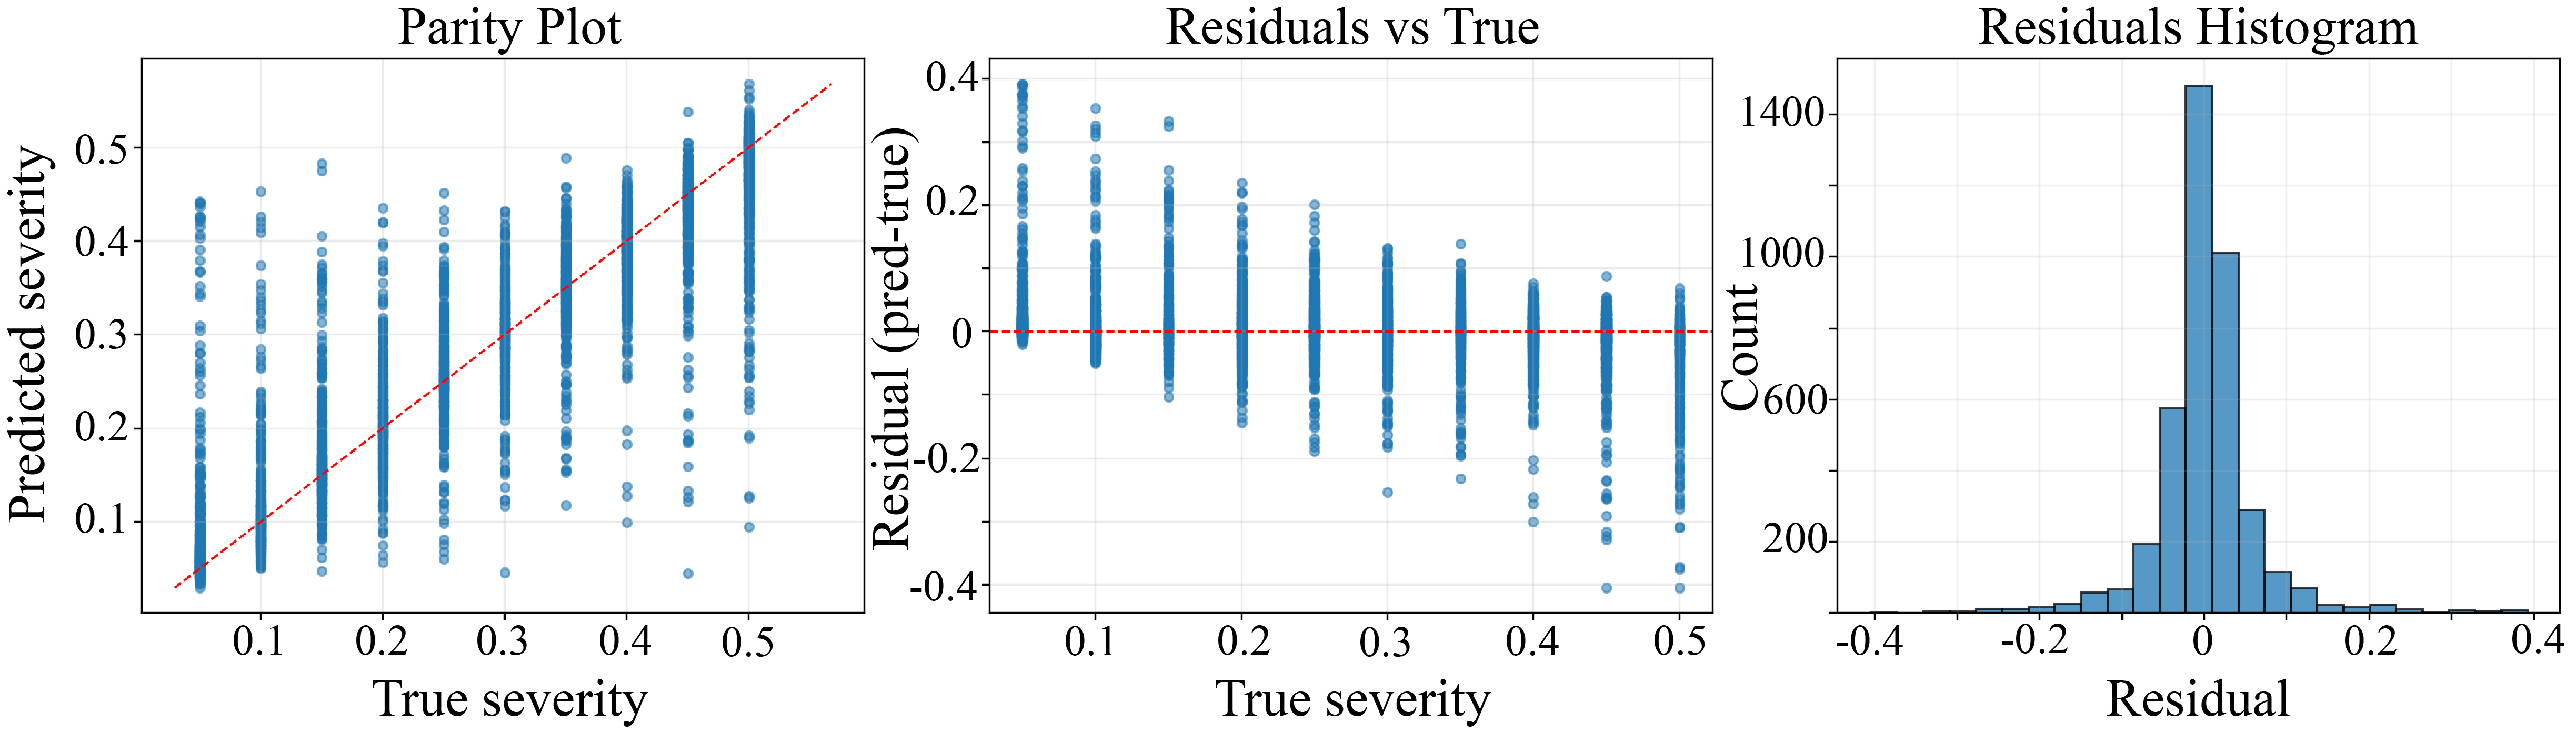
\includegraphics[width=0.98\columnwidth]{figs/severity_reg_attack_pcc_diagnostics_revise.png}

%     \vspace{0.3em}
%     \textbf{(b)} PCC-side stream

%     \caption{Attack-only severity-regression diagnostics for the motor-side and PCC-side streams. Panel (a) shows the motor-side results, while panel (b) shows the PCC-side results.}
%     \label{fig:app_regression_diagnostics}
% \end{figure}

\end{document}

